%! program = pdflatex

\documentclass[12pt]{article}

%%% PACKAGES
\usepackage{ifpdf}
\usepackage{booktabs}   % for much better looking tables
\usepackage{array}      % for better arrays (eg matrices) in maths
\usepackage{paralist}   % very flexible & customisable lists (eg. enumerate/itemize, etc.)
%\usepackage{verbatim}   % adds environment for commenting out blocks of text & for better verbatim
\usepackage{subfigure}  % make it possible to include more than one captioned figure/table in a single float
% These packages are all incorporated in the memoir class to one degree or another...
\ifpdf
\usepackage[pdftex]{graphicx}
\else
\usepackage[dvips]{graphicx}
\fi
\usepackage{epstopdf}
\usepackage[cmex10]{amsmath}
\interdisplaylinepenalty=2500

%%% PAGE DIMENSIONS
\usepackage{geometry} % to change the page dimensions
\geometry{letterpaper}
%\geometry{margins=2in} % for example, change the margins to 2 inches all round
%\geometry{landscape} % set up the page for landscape
% read geometry.pdf for detailed page layout information

%% HEADERS & FOOTERS
\usepackage{fancyhdr} % This should be set AFTER setting up the page geometry
\pagestyle{fancy} % options: empty , plain , fancy
\renewcommand{\headrulewidth}{0pt} % customise the layout...
%\lhead{}\chead{}\rhead{\hl{--- DRAFT ---}}
\lhead{}\chead{}\rhead{}
\lfoot{}\cfoot{\thepage}\rfoot{}

% *** MY ADDITIONAL PACKAGES ***
\usepackage{amsfonts}
\usepackage{amstext}
%\usepackage{ctable}        % messes up table captions among other things
\usepackage{booktabs}       % defines \toprule, \midrule, \bottomrule
\usepackage{threeparttable} % needed for table notes
\usepackage{longtable}      % for multi-page tables
\usepackage[font=normalsize]{caption}   % to keep caption for multi-page
                            % table normal size after using \footnotesize
                            % to reduce rest of table
%\usepackage{multirow}
%\usepackage{mathenv}
\usepackage{textcomp}      % improves \textregistered, provides \textquotesingle
\usepackage[usenames]{color}
\usepackage{soul}
\usepackage{fancyvrb}
\usepackage{relsize}
\usepackage[noadjust]{cite} % prevent adding a space
%\usepackage{url}
\usepackage{xr-hyper}
\usepackage[usenames,dvipsnames,svgnames,table]{xcolor} % additional named colors
\usepackage[colorlinks=true,urlcolor=blue,hyperfootnotes=false,backref=section,citecolor=LimeGreen]{hyperref}
%\usepackage[colorlinks=true,urlcolor=blue,hyperfootnotes=false]{hyperref}
% These are (supposedly) the defaults
% \hypersetup{
%     bookmarks=true,         % show bookmarks bar?
%     unicode=false,          % non-Latin characters in Acrobat's bookmarks
%     pdftoolbar=true,        % show Acrobat's toolbar?
%     pdfmenubar=true,        % show Acrobat's menu?
%     pdffitwindow=true,      % page fit to window when opened
%     pdftitle={My title},    % title
%     pdfauthor={Author},     % author
%     pdfsubject={Subject},   % subject of the document
%     pdfcreator={Creator},   % creator of the document
%     pdfproducer={Producer}, % producer of the document
%     pdfkeywords={keywords}, % list of keywords
%     pdfnewwindow=true,      % links in new window
%     colorlinks=false,       % false: boxed links; true: colored links
%     linkcolor=red,          % color of internal links
%     citecolor=green,        % color of links to bibliography
%     filecolor=magenta,      % color of file links
%     urlcolor=cyan           % color of external links
% }
\usepackage{upquote}        % single quotes in verbatim environments
\usepackage[title,titletoc]{appendix}

%%% SECTION TITLE APPEARANCE
% \usepackage{sectsty}
% \allsectionsfont{\sffamily\mdseries\upshape} % (See the fntguide.pdf for font help)
% (This matches ConTeXt defaults)

%%% ToC APPEARANCE
\usepackage[nottoc,notlof,notlot]{tocbibind} % Put the bibliography in the ToC
% \usepackage[titles]{tocloft} % Alter the style of the Table of Contents
% \renewcommand{\cftsecfont}{\rmfamily\mdseries\upshape}
% \renewcommand{\cftsecpagefont}{\rmfamily\mdseries\upshape} % No bold!

% Namelist environment generates a list with an item width of your choice.
% Syntax:  \begin{namelist}{widthstring} .  From Buerger's book.
\newcommand{\namelistlabel}[1]{\mbox{#1}\hfil}
\newenvironment{namelist}[1]{%
\begin{list}{}
  {
    \let\makelabel\namelistlabel
    \settowidth{\labelwidth}{#1}
    \setlength{\leftmargin}{1.1\labelwidth}
  }
 }{%
\end{list}}

% define my verbatim environment, requires packages fancyvrb & relsize
\renewcommand{\FancyVerbFormatLine}[1]{\makebox[2mm][l]{}#1}
\DefineVerbatimEnvironment%
  {Code}{Verbatim}
  {fontsize=\relsize{-1.5},
  samepage=true,
  frame=single}

% define my verbatim environment, requires packages fancyvrb & relsize
\renewcommand{\FancyVerbFormatLine}[1]{\makebox[2mm][l]{}#1}
\DefineVerbatimEnvironment%
  {Notice}{Verbatim}
  {fontsize=\relsize{-1.5},
  samepage=true,
  xleftmargin=15mm,
  framesep=5mm,
  frame=single}

%% makes verbatim text 'small' (using verbatim package)
%\makeatletter
%\g@addto@macro\@verbatim\small
%\makeatother

%\hyphenation{matpower_manual}

\newcommand{\mpver}[0]{8.0}
%\newcommand{\matlab}[0]{{Matlab}}
%\newcommand{\matlab}[0]{{\sc Matlab}\textsuperscript{\tiny \textregistered}}
\newcommand{\matlab}[0]{{\sc Matlab}}
\newcommand{\matpower}[0]{{\sc Matpower}}
\newcommand{\matpowerurl}[0]{https://matpower.org}
\newcommand{\matpowerlink}[0]{\href{\matpowerurl}{\matpower{}}}
\newcommand{\matpowergithuburl}[0]{https://github.com/MATPOWER/matpower}
\newcommand{\mptest}[0]{{MP-Test}}
\newcommand{\mptesturl}[0]{https://github.com/MATPOWER/mptest}
\newcommand{\mptestlink}[0]{\href{\mptesturl}{\mptest{}}}
\newcommand{\mptestver}[0]{8.0}
\newcommand{\mips}[0]{{MIPS}}
\newcommand{\mipsurl}[0]{https://github.com/MATPOWER/mips}
\newcommand{\mipslink}[0]{\href{\mipsurl}{\mips{}}}
\newcommand{\mipsname}[0]{{{\bf M}{\sc atpower} \textbf{I}nterior \textbf{P}oint \textbf{S}olver}}
\newcommand{\mipsver}[0]{1.5.1}
\newcommand{\mpom}[0]{\mbox{MP-Opt-Model}}
\newcommand{\mpomurl}[0]{https://github.com/MATPOWER/mp-opt-model}
\newcommand{\mpomlink}[0]{\href{\mpomurl}{\mpom{}}}
\newcommand{\mpomname}[0]{\mpom{}}
% \newcommand{\mpomname}[0]{{{\bf M}{\sc at}{\bf P}{\sc ower} \textbf{Opt}imization \textbf{Model}}}
\newcommand{\mpomver}[0]{5.0-dev}
\newcommand{\most}[0]{{MOST}}
\newcommand{\mostname}[0]{{{\bf M}{\sc atpower} \textbf{O}ptimal \textbf{S}cheduling \textbf{T}ool}}
\newcommand{\mosturl}[0]{https://github.com/MATPOWER/most}
\newcommand{\mostlink}[0]{\href{\mosturl}{\most{}}}
\newcommand{\mostver}[0]{1.3}
\newcommand{\syngrid}[0]{{SynGrid}}
\newcommand{\syngridver}[0]{1.0.1}
\newcommand{\syngridurl}[0]{https://github.com/MATPOWER/mx-syngrid}
\newcommand{\syngridlink}[0]{\href{\syngridurl}{\syngrid{}}}
\newcommand{\md}[0]{{\most{} Data struct}}
\newcommand{\powerweb}[0]{{\sc PowerWeb}}
\newcommand{\pserc}[0]{{\sc PSerc}}
\newcommand{\PSERC}[0]{{Power Systems Engineering Research Center (\pserc{})}}
\newcommand{\certs}[0]{{\sc Certs}}
\newcommand{\CERTS}[0]{{Consortium for Electric Reliability Technology Solutions (\certs{})}}
\newcommand{\ipopt}[0]{{\sc Ipopt}}
\newcommand{\knitro}[0]{{Artelys Knitro}}
\newcommand{\clp}[0]{{CLP}}
\newcommand{\cplex}[0]{{CPLEX}}
\newcommand{\glpk}[0]{{GLPK}}
\newcommand{\gurobi}[0]{{Gurobi}}
\newcommand{\highs}[0]{{HiGHS}}
\newcommand{\mosek}[0]{{MOSEK}}
\newcommand{\osqp}[0]{{OSQP}}
\newcommand{\osqplink}[0]{{\href{https://osqp.org}{\osqp}}}
\newcommand{\ot}[0]{{Optimization Toolbox}}
\newcommand{\pardiso}[0]{{PARDISO}}
\newcommand{\sdppf}[0]{\texttt{SDP\_PF}}
\newcommand{\sdppfver}[0]{1.0.2}
\newcommand{\sdpopf}[0]{SDPOPF}
\newcommand{\code}[1]{{\relsize{-0.5}{\tt{{#1}}}}}  % requires package relsize
% Note: to get straight single quotes in \code you have to use one of the
%       following: \char13 \char'15 \char"0D \textquotesingle
\newcommand{\codeq}[1]{\code{\textquotesingle{}#1\textquotesingle}}  % requires package textcomp
\newcommand{\mppath}[1]{\textsf{\textsl{{\relsize{-1.0}\textless{}\mbox{MATPOWER}\textgreater{}}}}\code{{#1}}}  % requires package relsize
%\newcommand{\mostpath}[1]{\code{\$MOST{#1}}}
\newcommand{\mipspath}[1]{\textsf{\textsl{{\relsize{-1.0}\textless{}\mbox{MIPS}\textgreater{}}}}\code{{#1}}}  % requires package relsize
\newcommand{\mpompath}[1]{\textsf{\textsl{{\relsize{-1.0}\textless{}\mbox{MPOM}\textgreater{}}}}\code{{#1}}}  % requires package relsize
\newcommand{\mostpath}[1]{\mppath{}\code{/most{#1}}}
\newcommand{\baseMVA}[0]{\code{baseMVA}}
\newcommand{\bus}[0]{\code{bus}}
\newcommand{\branch}[0]{\code{branch}}
\newcommand{\gen}[0]{\code{gen}}
\newcommand{\gencost}[0]{\code{gencost}}
\newcommand{\areas}[0]{\code{areas}}
\newcommand{\mpc}[0]{\code{mpc}}
\newcommand{\results}[0]{\code{results}}
\newcommand{\mumurl}[0]{https://matpower.org/docs/MATPOWER-manual-\mpver.pdf}
\newcommand{\mum}[0]{\href{\mumurl}{\matpower{} User's Manual}}
\newcommand{\mipsmanurl}[0]{https://matpower.org/docs/MIPS-manual-\mipsver.pdf}
\newcommand{\mpommanurl}[0]{https://matpower.org/docs/MP-Opt-Model-manual-\mpomver.pdf}
\newcommand{\mostmanurl}[0]{https://matpower.org/docs/MOST-manual-\mostver.pdf}
\newcommand{\currentmumurl}[0]{https://matpower.org/docs/MATPOWER-manual.pdf}
\newcommand{\currentmipsmanurl}[0]{https://matpower.org/docs/MIPS-manual.pdf}
\newcommand{\currentmpommanurl}[0]{https://matpower.org/docs/MP-Opt-Model-manual.pdf}
\newcommand{\currentmostmanurl}[0]{https://matpower.org/docs/MOST-manual.pdf}
\newcommand{\mipsman}[0]{\href{\mipsmanurl}{\mips{} User's Manual}}
\newcommand{\mpomman}[0]{\href{\mpommanurl}{\mpom{} User's Manual}}
\newcommand{\mostman}[0]{\href{\mostmanurl}{\most{} User's Manual}}
\newcommand{\dg}[0]{\sp\dagger}                         % hermitian conjugate
\newcommand{\trans}[1]{{#1}^{\ensuremath{\mathsf{T}}}}  % transpose
%\newcommand{\trans}[1]{#1^{\ensuremath{\mathsf{T}}}}    % transpose
\newcommand{\cc}[1]{{#1}^{\ast}}                        % complex conjugate
\newcommand{\hc}[1]{{#1}^{\dg}}                         % hermitian conjugate
\newcommand{\conj}[1]{{#1}^{+}}                         % hermitian conjugate
\newcommand{\diag}[1]{\left[{#1}\right]}                % diagonal
\newcommand{\R}{\mathbb{R}}          % requires \usepackage{amsfonts|bbold}
\newcommand{\der}[2]{\frac{\partial{#1}}{\partial{#2}}} % partial derivative
\newcommand{\doi}[1]{doi:~\href{https://doi.org/#1}{#1}}

\newcommand{\llq}{l_\textrm{q}}
\newcommand{\uuq}{u_\textrm{q}}
\newcommand{\llqi}{{l_\textrm{q}}_i}
\newcommand{\uuqi}{{u_\textrm{q}}_i}

\def\sectionautorefname{Chapter}
\def\subsectionautorefname{Section}
\def\subsubsectionautorefname{Section}
\newcommand{\secref}[1]{\autoref{#1} \nameref{#1}}

\numberwithin{equation}{section}
\numberwithin{table}{section}
\renewcommand{\thetable}{\thesection\mbox{-}\arabic{table}}
\numberwithin{figure}{section}
\renewcommand{\thefigure}{\thesection\mbox{-}\arabic{figure}}

\externaldocument[MIPSMAN-]{MIPS-manual}[\mipsmanurl]
% \externaldocument[MOSTMAN-]{MOST-manual}[\mostmanurl]


%\title{\hl{--- DRAFT  ---}\\\hl{\em do not distribute}\\~\\{\huge \bfseries \mpomname{} User's Manual } \\ ~ \\ \LARGE Version \mpomver{}\\
\title{{\huge \bfseries \mpomname{} User's Manual } \\ ~ \\ \LARGE Version \mpomver{}}
\author{Ray~D.~Zimmerman}
%\date{May 10, 2024} % comment this line to display the current date
%\date{May 8, 2020\thanks{Second revision. First revision was April 29, 2020}} % comment this line to display the current date

%%% BEGIN DOCUMENT
\begin{document}

\maketitle
\thispagestyle{empty}
\vfill
\begin{center}
{\scriptsize
\copyright~2020--2025~\PSERC{}\\
All Rights Reserved}
\end{center}

\clearpage
%\setcounter{page}{2}
\tableofcontents
\clearpage
%\listoffigures
\listoftables

%%------------------------------------------
\clearpage
\section{Introduction}

\subsection{Background}

\mpomlink{} is a package of \matlab{} language M-files\footnote{Also compatible with GNU Octave~\cite{octave}.} for constructing and solving mathematical programming and optimization problems. It provides an easy-to-use, object-oriented interface for building and solving your model. It also includes a unified interface for calling numerous LP, QP, QCQP, mixed-integer, and nonlinear solvers, with the ability to switch solvers simply by changing an input option.
The \mpom{} project page can be found at:

\bigskip

~~~~~~~~\url{\mpomurl}

\bigskip

\mpomlink{} is based on code that was developed primarily by Ray~D.~Zimmerman of \pserc{}\footnote{\url{http://pserc.org/}} at Cornell University, along with significant contributions from others, as part of the \matpowerlink{}~\cite{zimmerman2011,matpower} project.

Up until version 7 of \matpower{}, the code now included in \mpom{} was distributed only as an integrated part of \matpower{}. After the release of \matpower{} 7, \mpom{} was split out into a separate project, though it is still included with \matpower{}.

\clearpage
\subsection{License and Terms of Use}

The code in \mpom{} is distributed under the 3-clause BSD license
~\cite{bsd}. The full text of the license can be found in the \code{LICENSE} file at the top level of the distribution or at \url{https://github.com/MATPOWER/mp-opt-model/blob/master/LICENSE} and reads as follows.

\begin{Notice}
Copyright (c) 2004-2024, Power Systems Engineering Research Center
(PSERC) and individual contributors (see AUTHORS file for details).
All rights reserved.

Redistribution and use in source and binary forms, with or without
modification, are permitted provided that the following conditions
are met:

1. Redistributions of source code must retain the above copyright
notice, this list of conditions and the following disclaimer.

2. Redistributions in binary form must reproduce the above copyright
notice, this list of conditions and the following disclaimer in the
documentation and/or other materials provided with the distribution.

3. Neither the name of the copyright holder nor the names of its
contributors may be used to endorse or promote products derived from
this software without specific prior written permission.

THIS SOFTWARE IS PROVIDED BY THE COPYRIGHT HOLDERS AND CONTRIBUTORS
"AS IS" AND ANY EXPRESS OR IMPLIED WARRANTIES, INCLUDING, BUT NOT
LIMITED TO, THE IMPLIED WARRANTIES OF MERCHANTABILITY AND FITNESS
FOR A PARTICULAR PURPOSE ARE DISCLAIMED. IN NO EVENT SHALL THE
COPYRIGHT HOLDER OR CONTRIBUTORS BE LIABLE FOR ANY DIRECT, INDIRECT,
INCIDENTAL, SPECIAL, EXEMPLARY, OR CONSEQUENTIAL DAMAGES (INCLUDING,
BUT NOT LIMITED TO, PROCUREMENT OF SUBSTITUTE GOODS OR SERVICES;
LOSS OF USE, DATA, OR PROFITS; OR BUSINESS INTERRUPTION) HOWEVER
CAUSED AND ON ANY THEORY OF LIABILITY, WHETHER IN CONTRACT, STRICT
LIABILITY, OR TORT (INCLUDING NEGLIGENCE OR OTHERWISE) ARISING IN
ANY WAY OUT OF THE USE OF THIS SOFTWARE, EVEN IF ADVISED OF THE
POSSIBILITY OF SUCH DAMAGE.
\end{Notice}

\clearpage
\subsection{Citing \mpom{}}

We request that publications derived from the use of \mpom{} explicitly acknowledge that fact by citing the \mpomname{} User's Manual~\cite{mpom_manual}.
The citation and DOI can be version-specific or general, as appropriate. For version 4.2, use:

\begin{quote}
\footnotesize
R.~D. Zimmerman. \mpomname{} User's Manual, Version 4.2. 2024. [Online]. Available: \url{https://matpower.org/docs/MP-Opt-Model-manual-4.2.pdf}\\
\doi{10.5281/zenodo.11177079}
\end{quote}
For a version non-specific citation, use the following citation and DOI,
with \emph{\textless{}YEAR\textgreater{}} replaced by the year of the most recent release:

\begin{quote}
\footnotesize
R.~D. Zimmerman. \mpomname{} User's Manual. \emph{\textless{}YEAR\textgreater{}}.
[Online]. Available: \url{https://matpower.org/docs/MP-Opt-Model-manual.pdf}\\
\doi{10.5281/zenodo.3818002}
\end{quote}
A list of versions of the User's Manual with release dates and
version-specific DOI's can be found via the general DOI at
\url{https://doi.org/10.5281/zenodo.3818002}.

\subsection{\mpom{} Development}
\label{sec:development}

The \mpom{} project uses an open development paradigm, hosted on the \mpom{} GitHub project page:

\bigskip

~~~~~~~~\url{\mpomurl}

\bigskip

The \mpom{} GitHub project hosts the public Git code repository as well as a public issue tracker for handling bug reports, patches, and other issues and contributions. There are separate GitHub hosted repositories and issue trackers for \mpom{}, \mptest{}, \mips{}, and \matpower{}, etc., all are available from \url{https://github.com/MATPOWER/}.


%%------------------------------------------
\clearpage
\section{Getting Started}

% Note: MATLAB 7.5 is the first version to support including prototypes
% for external methods in classdef, used by mp_idx_manager.
% Octave 3.8.2 does not support some of the OO syntax we use.

\subsection{System Requirements}
\label{sec:sysreq}
To use \mpom{} \mpomver{} you will need:
\begin{itemize}
\item \matlab{}\textsuperscript{\tiny \textregistered} version 7.9 (R2009b) or later\footnote{\matlab{} is available from The MathWorks, Inc. (\url{https://www.mathworks.com/}). \matlab{} is a registered trademark of The MathWorks, Inc.}, or
\item GNU Octave version 6.2 or later\footnote{GNU Octave \cite{octave} is free software, available online at \url{https://octave.org}. All functionality except object copy constructors work on GNU Octave version
4.4 and later. \mpom{}~4.2 and earlier required Octave~4.}
\item \mipslink{}, \mipsname{}~\cite{wang2007a, mips_manual}\footnote{\mips{} is available at \url{\mipsurl}.}
\item \mptestlink{}\footnote{\mptest{} is available at \url{\mptesturl}.}
\end{itemize}

For the hardware requirements, please refer to the system requirements for the version of \matlab{}\footnote{\url{https://www.mathworks.com/support/sysreq/previous_releases.html}} or Octave that you are using.

In this manual, references to \matlab{} usually apply to Octave as well.

%\clearpage
\subsection{Installation}
\label{sec:installation}

{\bf Note to \matpower{} users:} \emph{\mpom{} and its prerequisites, \mips{} and \mptest{}, are included when you install \matpower{}. There is generally no need to install \mpom{} separately. You can skip directly to step 3 to verify.}

~

Installation and use of \mpom{} requires familiarity with the basic operation of \matlab{} or Octave, including setting up your \matlab{}/Octave path.

\begin{enumerate}[\bfseries Step 1:] % requires package paralist
\item Clone the repository or download and extract the zip file of the \mpom{} distribution from the \href{\mpomurl{}}{\mpom{} project page}\footnote{\url{\mpomurl}} to the location of your choice. The files in the resulting \code{mp-opt-model} or \code{mp-opt-modelXXX} directory, where \code{XXX} depends on the version of \mpom{}, should not need to be modified, so it is recommended that they be kept separate from your own code.
We will use \mpompath{} to denote the path to this directory.
\clearpage
\item Add the following directories to your \matlab{} or Octave path:
\begin{itemize}
\item \mpompath{/lib} -- core \mpom{} functions
\item \mpompath{/lib/t} -- test scripts for \mpom{}
\end{itemize}
\item At the \matlab{}/Octave prompt, type \code{test\_mp\_opt\_model} to run the test suite and verify that \mpom{} is properly installed and functioning.\footnote{The tests require functioning installations of \mptestlink{} and \mipslink{}.} The result should resemble the following:
%\clearpage
%--LATER--
%\\\hl{re-do before release (run on fastest machine available)}
\begin{Code}
>> test_mp_opt_model
t_have_fcn..............ok
t_nested_struct_copy....ok
t_nleqs_master..........ok (30 of 150 skipped)
t_pnes_master...........ok
t_qps_master............ok (100 of 432 skipped)
t_miqps_master..........ok (78 of 318 skipped)
t_nlps_master...........ok
t_opt_model.............ok
t_om_solve_leqs.........ok
t_om_solve_nleqs........ok (36 of 195 skipped)
t_om_solve_pne..........ok
t_om_solve_qps..........ok (81 of 388 skipped)
t_om_solve_miqps........ok (20 of 131 skipped)
t_om_solve_nlps.........ok
All tests successful (3461 passed, 345 skipped of 3806)
Elapsed time 2.28 seconds.
\end{Code}
\end{enumerate}


\subsection{Sample Usage}
\label{sec:usage}

Suppose we have the following constrained 4-dimensional quadratic programming (QP) problem with two 2-dimensional variables, $y$ and $z$, and two constraints, one equality and the other inequality, along with lower bounds on all of the variables.

\begin{equation}
\min_{y, z} \frac{1}{2} \left[\begin{array}{cc}\trans{y} & \trans{z} \end{array}\right] Q \left[\begin{array}{c}y \\ z \end{array}\right]
\end{equation}
subject to
\begin{align}
A_1 \left[\begin{array}{c}y \\ z \end{array}\right] &= b_1 \\
A_2 y &\le u_2 \\
y &\ge y_\mathrm{min} \\
z &\le z_\mathrm{max}
\end{align}

And suppose the data for the problem is provided as follows.

\begin{Code}
%% variable initial values
y0 = [1; 0];
z0 = [0; 1];

%% variable lower bounds
ymin = [0; 0];
zmax = [0; 2];

%% constraint data
A1 = [ 6 1 5 -4 ];  b1 = 4;
A2 = [ 4 9 ];       u2 = 2;

%% quadratic cost coefficients
Q = [ 8  1 -3 -4;
      1  4 -2 -1;
     -3 -2  5  4;
     -4 -1  4  12  ];
\end{Code}

Below, we will show two approaches to construct and solve the problem. The first method, based on the mathematical programming and optimization model class \code{mp.opt\_model}, allows you to add variables, constraints and costs to the model individually. Then \code{mp.opt\_model} automatically assembles and solves the full model automatically.

\begin{Code}
%%-----  METHOD 1  -----
%% build model
mm = mp.opt_model;
mm.var.add('y', 2, y0, ymin);
mm.var.add('z', 2, z0, [], zmax);
mm.lin.add(mm.var, 'lincon1', A1, b1, b1);
mm.lin.add(mm.var, 'lincon2', A2, [], u2, {'y'});
mm.qdc.add(mm.var, 'cost', Q, []);

%% solve model
[x, f, exitflag, output, lambda] = mm.solve();
\end{Code}

The second method requires you to construct the parameters for the full problem manually, then call the solver function directly.

\begin{Code}
%%-----  METHOD 2  -----
%% assemble model parameters manually
xmin = [ymin; -Inf(2,1)];
xmax = [ Inf(2,1); zmax];
x0 = [y0; z0];
A = [ A1; A2 0 0];
l = [ b1; -Inf ];
u = [ b1;  u2  ];

%% solve model
[x, f, exitflag, output, lambda] = qps_master(Q, [], A, l, u, xmin, xmax, x0);
\end{Code}

The above examples are included in \mpompath{lib/t/qp\_ex1.m} along with some commands to print the results, yielding the output below for each approach:

\begin{Code}
f = 1.875      exitflag = 1

             var bound shadow prices
     x     lambda.lower  lambda.upper
  0.5000      0.0000        0.0000
  0.0000      5.1250        0.0000
 -0.0000      0.0000        8.7500
 -0.2500      0.0000        0.0000

constraint shadow prices
lambda.mu_l  lambda.mu_u
  1.2500       0.0000
  0.0000       0.6250
\end{Code}

Both approaches can be applied to each of the types of problems that \mpom{} handles, namely, LP, QP, MILP, MIQP, QCQP, NLP and linear and nonlinear equations, including families of parameterized nonlinear equations.

An options struct can be passed to the \code{solve} method or the \code{qps\_master} function to select a specific solver, control the level of
progress output, or modify a solver's default parameters.

\clearpage
\subsection{Documentation}
\label{sec:documentation}

There are two primary sources of documentation for \mpom{}. The first is \href{\mpommanurl}{this manual}, which gives an overview of the capabilities and structure of \mpom{} and describes the formulations behind the code. It can be found in your \mpom{} distribution at \mpompath{/docs/MP-Opt-Model-manual.pdf} and the \href{\currentmpommanurl}{latest version} is always available at: \url{\currentmpommanurl}.

The second is the online \href{https://matpower.org/doc/mpom/}{\mpom{} Reference Manual}\footnote{\url{https://matpower.org/doc/mpom/}}, whose content is also available via the built-in \code{help} command. As with the built-in functions and toolbox routines in \matlab{} and Octave, you can type \code{help} followed by the name of a command or M-file to get help on that particular function. Many of the M-files in \mpom{} have such documentation and this should be considered the main reference for the calling options for each function. See Appendix~\ref{app:functions} for a list of \mpom{} functions.

%%------------------------------------------
\clearpage
\section{\mpom{} -- Overview}
\label{sec:mpom}

\mpom{}\footnote{The name \mpom{} was originally derived from ``\matpower{} Optimization Model,'' referring to the object used to encapsulate the optimization problem formed by \matpower{} when solving an optimal power flow (OPF) problem. However, given its subsequent expanded scope, it stands for ``Mathematical Programming and Optimization Model''} and its functionality can be divided into two main parts, plus a few additional utility functions.

The first part consists of interfaces to various numerical optimization solvers and the wrapper functions that provide a single common interface to all supported solvers for a particular class of problems. There is currently a common interface provided for each of the following:
\begin{itemize}
\item linear (LP) and quadratic (QP) programming problems
\item mixed-integer linear (MILP) and quadratic (MIQP) programming problems
\item quadratically-constrained quadratic programming problems (QCQP)
\item nonlinear programming problems (NLP)
\item linear equations (LEQ)
\item nonlinear equations (NLEQ)
\item parameterized nonlinear equations (PNE)
\end{itemize}

The second part consists of a mathematical programming and optimization model class designed to help the user construct an optimization or zero-finding problem by adding variables, constraints and/or costs, then solve the problem and extract the solution in terms of the individual sets of variables, constraints and/or costs provided.

Finally, \mpom{} includes a utlity function that can be used to get information about the availability of optional functionality, another to help with copying nested struct data, and a function that provides version information on the current \mpom{} installation.


%%------------------------------------------
\clearpage
\section{Solver Interface Functions}
\label{sec:master_solvers}

\subsection{LP/QP Solvers -- {\tt qps\_master}}
\label{sec:qps_master}

The \code{qps\_master} function provides a common \textbf{\underline{q}}uadratic \textbf{\underline{p}}rogramming \textbf{\underline{s}}olver interface for linear programming (LP) and quadratic (QP) programming problems, that is, problems of the form:
\begin{equation}
\min_x \frac{1}{2} \trans{x} H x + \trans{c} x \label{eq:QPobj}
\end{equation}
subject to
\begin{eqnarray}
& l \le A x \le u  & \\
& x_\mathrm{min} \le x \le x_\mathrm{max}. & \label{eq:QPvarbounds}
\end{eqnarray}

This function can be used to solve the problem with any of the available solvers by calling it as follows,
\begin{Code}
[x, f, exitflag, output, lambda] = ...
    qps_master(H, c, A, l, u, xmin, xmax, x0, opt);
\end{Code}
where the input and output arguments are described in Tables~\ref{tab:qps_master_input} and \ref{tab:qps_master_output}, respectively, and the options in Table~\ref{tab:qps_master_options}.
Alternatively, the input arguments can be packaged as fields in a \code{problem} struct and passed in as a single argument, where all fields are (individually) optional.
\begin{Code}
[x, f, exitflag, output, lambda] = qps_master(problem);
\end{Code}

The calling syntax is very similar to that used by \code{quadprog} from the \matlab{} \ot{}, with the primary difference that the linear constraints are specified in terms of a single doubly-bounded linear function ($l \le A x \le u$) as opposed to separate equality constrained ($A_{eq} x = b_{eq}$) and upper bounded ($A x \le b$) functions.

\begin{table}[!ht]
%\renewcommand{\arraystretch}{1.2}
\centering
\begin{threeparttable}
\caption{Input Arguments for \code{qps\_master}\tnote{\dag}}
\label{tab:qps_master_input}
\footnotesize
% \begin{tabular}{p{0.17\textwidth}p{0.76\textwidth}}
\begin{tabular}{ll}
\toprule
name & description \\
\midrule
\code{H}	& (possibly sparse) matrix $H$ of quadratic cost coefficients	\\
\code{c}	& column vector $c$ of linear cost coefficients	\\
\code{A}	& (possibly sparse) matrix $A$ of linear constraint coefficients	\\
\code{l}	& column vector $l$ of lower bounds on $A x$, defaults to $-\infty$	\\
\code{u}	& column vector $u$ of upper bounds on $A x$, defaults to $+\infty$	\\
\code{xmin}	& column vector $x_\mathrm{min}$ of lower bounds on $x$, defaults to $-\infty$	\\
\code{xmax}	& 	column vector $x_\mathrm{max}$ of upper bounds on $x$, defaults to $+\infty$	\\
\code{x0}	& optional starting value of optimization vector $x$ \emph{(ignored by some solvers)}	\\
\code{opt}	& optional options struct (all fields optional), see Table~\ref{tab:qps_master_options} for details	\\
\code{problem}	& alternative, single argument input struct with fields corresponding to arguments above	\\
\bottomrule
\end{tabular}
\begin{tablenotes}
 \scriptsize
 \item [\dag] {All arguments are individually optional, though enough must be supplied to define a meaningful problem.}
\end{tablenotes}
\end{threeparttable}
\end{table}

\begin{table}[!ht]
%\renewcommand{\arraystretch}{1.2}
\centering
\begin{threeparttable}
\caption{Output Arguments for \code{qps\_master}}
\label{tab:qps_master_output}
\footnotesize
\begin{tabular}{p{0.12\textwidth}p{0.82\textwidth}}
\toprule
name & description \\
\midrule
\code{x}	& solution vector $x$	\\
\code{f}	& final objective function value $f(x) = \frac{1}{2} \trans{x} H x + \trans{c} x$	\\
\code{exitflag}	& exit flag	\\
& \begin{tabular}{r @{ -- } l}
1 & converged successfully \\
$\le 0$ & solver-specific failure code \\
\end{tabular}	\\
\code{output}	& output struct with the following fields:	\\
& \begin{tabular}{r @{ -- } l}
\code{alg} & algorithm code of solver used \\
\emph{(others)} & solver-specific fields \\
\end{tabular}	\\
\code{lambda}	& struct containing the Langrange and Kuhn-Tucker multipliers on the constraints, with fields:	\\
& \begin{tabular}{r @{ -- } l}
\code{mu\_l} & lower (left-hand) limit on linear constraints \\
\code{mu\_u} & upper (right-hand) limit on linear constraints \\
\code{lower} & lower bound on optimization variables \\
\code{upper} & upper bound on optimization variables \\
\end{tabular}	\\
\bottomrule
\end{tabular}
% \begin{tablenotes}
%  \scriptsize
%  \item [\dag] {Requires the installation of an optional package. See Appendix~\ref{app:optional_packages} for details on the corresponding package.}
% \end{tablenotes}
\end{threeparttable}
\end{table}

\begin{table}[!ht]
%\renewcommand{\arraystretch}{1.2}
\centering
\begin{threeparttable}
\caption{Options for \code{qps\_master}}
\label{tab:qps_master_options}
\footnotesize
\begin{tabular}{lcp{0.62\textwidth}}
\toprule
name & default & description \\
\midrule
\code{alg}	& \codeq{DEFAULT}	& determines which solver to use \\
&& \begin{tabular}{c @{ -- } p{0.5\textwidth}}
\codeq{DEFAULT} & automatic, first available of \gurobi{}, \cplex{}, \mosek{}, \ot{} (if \matlab{}), \highs{}, \glpk{} (LP only), BPMPD, \mips{} \\
\codeq{BPMPD} & BPMPD\tnote{*} \\
\codeq{CLP} & \clp{}\tnote{*} \\
\codeq{CPLEX} & \cplex{}\tnote{*} \\
\codeq{GLPK} & \glpk{}\tnote{*} \emph{(LP only)} \\
\codeq{GUROBI} & \gurobi{}\tnote{*} \\
\codeq{HIGHS} & \highs{}\tnote{*} \\
\codeq{IPOPT} & \ipopt{}\tnote{*} \\
\codeq{MIPS} & \mipslink{}, \mipsname{} \\
\codeq{MOSEK} & \mosek{}\tnote{*} \\
\codeq{OT} & \matlab{} Opt Toolbox, \code{quadprog}, \code{linprog} \\
\end{tabular}	\\
\code{verbose}	& 0	& amount of progress info to be printed \\
&& \begin{tabular}{r @{ -- } l}
0 & print no progress info \\
1 & print a little progress info \\
2 & print a lot of progress info \\
3 & print all progress info \\
\end{tabular}	\\
\code{bp\_opt}	& \emph{empty}	& options vector for \code{bp}\tnote{*} \\
\code{clp\_opt}	& \emph{empty}	& options vector for \clp{}\tnote{*} \\
\code{cplex\_opt}	& \emph{empty}	& options struct for \cplex{}\tnote{*} \\
\code{glpk\_opt}	& \emph{empty}	& options struct for \glpk{}\tnote{*} \\
\code{grb\_opt}	& \emph{empty}	& options struct for \gurobi{}\tnote{*} \\
\code{highs\_opt}	& \emph{empty}	& options struct for \highs{}\tnote{*} \\
\code{ipopt\_opt}	& \emph{empty}	& options struct for \ipopt{}\tnote{*} \\
\code{linprog\_opt}	& \emph{empty}	& options struct for \code{linprog}\tnote{*} \\
\code{mips\_opt}	& \emph{empty}	& options struct for \mips{} \\
\code{mosek\_opt}	& \emph{empty}	& options struct for \mosek{}\tnote{*} \\
\code{quadprog\_opt}	& \emph{empty}	& options struct for \code{quadprog}\tnote{*} \\
\bottomrule
\end{tabular}
\begin{tablenotes}
 \scriptsize
 \item [*] {Requires the installation of an optional package. See Appendix~\ref{app:optional_packages} for details on the corresponding package.}
\end{tablenotes}
\end{threeparttable}
\end{table}

The \code{qps\_master} function is simply a master wrapper around corresponding functions specific to each solver, namely, \code{qps\_bpmpd}, \code{qps\_clp}, \code{qps\_cplex}, \code{qps\_glpk}, \code{qps\_gurobi}, \code{qps\_highs}, \code{qps\_ipopt}, \code{qps\_knitro}, \code{qps\_mips}, \code{qps\_mosek}, and \code{qps\_ot}. Each of these functions has an interface identical to that of \code{qps\_master}, with the exception of the options struct for \code{qps\_mips}, which is a simple \mips{} options struct.

\clearpage
\subsubsection{QP Example}
\label{sec:qp_ex}

The following code shows an example of using \code{qps\_master} to solve a simple 4-dimensional QP problem\footnote{From \url{https://v8doc.sas.com/sashtml/iml/chap8/sect12.htm}.} using the default solver.

\begin{Code}
H = [   1003.1  4.3     6.3     5.9;
        4.3     2.2     2.1     3.9;
        6.3     2.1     3.5     4.8;
        5.9     3.9     4.8     10  ];
c = zeros(4,1);
A = [   1       1       1       1;
        0.17    0.11    0.10    0.18    ];
l = [1; 0.10];
u = [1; Inf];
xmin = zeros(4,1);
x0 = [1; 0; 0; 1];
opt = struct('verbose', 2);
[x, f, s, out, lambda] = qps_master(H, c, A, l, u, xmin, [], x0, opt);
\end{Code}

Other examples of using \code{qps\_master} to solve LP and QP problems can be found in \code{t\_qps\_master.m}.


\clearpage
\subsection{MILP/MIQP Solvers -- {\tt miqps\_master}}
\label{sec:miqps_master}

The \code{miqps\_master} function provides a common \textbf{\underline{m}}ixed-\textbf{\underline{i}}nteger \textbf{\underline{q}}uadratic \textbf{\underline{p}}rogramming \textbf{\underline{s}}olver interface for mixed-integer linear programming (MILP) and mixed-integer quadratic programming (MIQP) problems. The form of the problem is identical to \eqref{eq:QPobj}--\eqref{eq:QPvarbounds}, with the addition of two possible additional constraints, namely,
\begin{align}
x_i \in \mathbb{Z}, \qquad\quad \forall i &\in \mathcal{I} \label{eq:mi_integer}\\
x_j \in \{0, 1\}, \quad \forall j &\in \mathcal{B}, \label{eq:mi_binary}
\end{align}
where $\mathcal{I}$ and $\mathcal{B}$ are the sets of indices of variables that are restricted to integer or binary values, respectively.

This function can be used to solve the problem with any of the available solvers by calling it as follows,
\begin{Code}
[x, f, exitflag, output, lambda] = ...
    miqps_master(H, c, A, l, u, xmin, xmax, x0, vtype, opt);
[x, f, exitflag, output, lambda] = miqps_master(problem);
\end{Code}
The calling syntax for \code{miqps\_master} is identical to that used by \code{qps\_master} with the exception of a single new input argument, \code{vtype}, to specify the variable type, just before the options struct. The input arguments and options for \code{miqps\_master} are described in Tables~\ref{tab:miqps_master_input} and \ref{tab:miqps_master_options}, respectively. The outputs are identical to those shown in Table~\ref{tab:qps_master_output} for \code{qps\_master}.


\begin{table}[!ht]
%\renewcommand{\arraystretch}{1.2}
\centering
\begin{threeparttable}
\caption{Input Arguments for \code{miqps\_master}}
\label{tab:miqps_master_input}
\footnotesize
\begin{tabular}{p{0.15\textwidth}p{0.78\textwidth}}
\toprule
name & description \\
\midrule
\multicolumn{2}{l}{\emph{all \code{qps\_master} input args from Table~\ref{tab:qps_master_input}, with the following additions/modifications}} \\
& \\
\code{vtype}	& character string of length $n_x$ (number of elements in $x$), or 1 (value applies to all variables in $x$), specifying variable type; allowed values are:\tnote{\dag}	\\
& \begin{tabular}{r @{ -- } l}
\codeq{C} & continuous (default) \\
\codeq{B} & binary \\
\codeq{I} & integer \\
\end{tabular}	\\
\bottomrule
\end{tabular}
\begin{tablenotes}
 \scriptsize
 \item [\dag] {\cplex{} and \gurobi{} also include \codeq{S} for semi-continuous and \codeq{N} for semi-integer, but these have not been tested.}
\end{tablenotes}
\end{threeparttable}
\end{table}

% \begin{table}[!ht]
% %\renewcommand{\arraystretch}{1.2}
% \centering
% \begin{threeparttable}
% \caption{Output Arguments for \code{miqps\_master}\tnote{\dag}}
% \label{tab:miqps_master_output}
% \footnotesize
% \begin{tabular}{p{0.15\textwidth}p{0.78\textwidth}}
% \toprule
% name & description \\
% \midrule
% \multicolumn{2}{l}{\emph{all \code{qps\_master} output args from Table~\ref{tab:qps_master_output}, with the following additions/modifications}} \\
% & \\
% \code{x}	& solution vector $x$	\\
% \code{f}	& final objective function value $f(x) = \frac{1}{2} \trans{x} H x + \trans{c} x$	\\
% \code{exitflag}	& exit flag	\\
% & \begin{tabular}{r @{ -- } l}
% 1 & converged successfully \\
% $\le 0$ & solver-specific failure code \\
% \end{tabular}	\\
% \code{output}	& output struct with the following fields:	\\
% & \begin{tabular}{r @{ -- } l}
% \code{alg} & algorithm code of solver used \\
% \emph{(others)} & solver-specific fields \\
% \end{tabular}	\\
% \code{lambda}	& struct containing the Langrange and Kuhn-Tucker multipliers on the constraints, with fields:	\\
% & \begin{tabular}{r @{ -- } l}
% \code{mu\_l} & lower (left-hand) limit on linear constraints \\
% \code{mu\_u} & upper (right-hand) limit on linear constraints \\
% \code{lower} & lower bound on optimization variables \\
% \code{upper} & upper bound on optimization variables \\
% \end{tabular}	\\
% \bottomrule
% \end{tabular}
% % \begin{tablenotes}
% %  \scriptsize
% %  \item [\dag] {Requires the installation of an optional package. See Appendix~\ref{app:optional_packages} for details on the corresponding package.}
% % \end{tablenotes}
% \end{threeparttable}
% \end{table}


\begin{table}[!ht]
%\renewcommand{\arraystretch}{1.2}
\centering
\begin{threeparttable}
\caption{Options for \code{miqps\_master}}
\label{tab:miqps_master_options}
\footnotesize
\begin{tabular}{lcp{0.62\textwidth}}
\toprule
name & default & description \\
\midrule
% \multicolumn{3}{l}{\emph{all \code{qps\_master} options from Table~\ref{tab:qps_master_options}, with the following additions/modifications}} \\
% & \\
\code{alg}	& \codeq{DEFAULT}	& determines which solver to use \\
&& \begin{tabular}{c @{ -- } p{0.5\textwidth}}
\codeq{DEFAULT} & automatic, first available of \gurobi{}, \cplex{}, \mosek{}, \ot{} (if \matlab{}, MILP only), \highs{} (MILP only), \glpk{} (MILP only) \\
\codeq{CPLEX} & \cplex{}\tnote{*} \\
\codeq{GLPK} & \glpk{}\tnote{*} \emph{(LP only)} \\
\codeq{GUROBI} & \gurobi{}\tnote{*} \\
\codeq{HIGHS} & \highs{}\tnote{*} \\
\codeq{MOSEK} & \mosek{}\tnote{*} \\
\codeq{OT} & \matlab{} Opt Toolbox, \code{intlinprog} \\
\end{tabular}	\\
\code{verbose}	& 0	& amount of progress info to be printed \\
&& \begin{tabular}{r @{ -- } l}
0 & print no progress info \\
1 & print a little progress info \\
2 & print a lot of progress info \\
3 & print all progress info \\
\end{tabular}	\\
\code{skip\_prices}	& 0	& flag that specifies whether or not to skip the price computation stage, in which the problem is re-solved for only the continuous variables, with all others being constrained to their solved values \\
\code{price\_stage\_warn\_tol}	& \emph{$10^{-7}$}	& tolerance on the objective function value and primal variable relative mismatch required to avoid mismatch warning message \\
\code{cplex\_opt}	& \emph{empty}	& options struct for \cplex{}\tnote{*} \\
\code{glpk\_opt}	& \emph{empty}	& options struct for \glpk{}\tnote{*} \\
\code{grb\_opt}	& \emph{empty}	& options struct for \gurobi{}\tnote{*} \\
\code{highs\_opt}	& \emph{empty}	& options struct for \highs{}\tnote{*} \\
\code{intlinprog\_opt}	& \emph{empty}	& options struct for \code{intlinprog}\tnote{*} \\
\code{mosek\_opt}	& \emph{empty}	& options struct for \mosek{}\tnote{*} \\
\bottomrule
\end{tabular}
\begin{tablenotes}
 \scriptsize
 \item [*] {Requires the installation of an optional package. See Appendix~\ref{app:optional_packages} for details on the corresponding package.}
\end{tablenotes}
\end{threeparttable}
\end{table}

By default, unless the \code{skip\_prices} option is set to 1, once \code{miqps\_master} has found the integer solution, it constrain the integer variables to their solved values and call \code{qps\_matpower} on the resulting problem to determine the shadow prices in \code{lambda}.

The \code{miqps\_master} function is simply a master wrapper around corresponding functions specific to each solver, namely, \code{miqps\_cplex}, \code{miqps\_glpk}, \code{miqps\_gurobi}, \code{miqps\_highs}, \code{miqps\_mosek}, and \code{miqps\_ot}. Each of these functions has an interface identical to that of \code{miqps\_master}.

\clearpage
\subsubsection{MILP Example}
\label{sec:milp_ex}

The following code shows an example of using \code{miqps\_master} to solve a simple 2-dimensional MILP problem\footnote{From MOSEK 6.0 Guided Tour, section 7.13.1, \url{https://docs.mosek.com/6.0/toolbox/node009.html}.} using the default solver.

\begin{Code}
c = [-2; -3];
A = sparse([195 273; 4 40]);
u = [1365; 140];
xmax = [4; Inf];
vtype = 'I';
opt = struct('verbose', 2);
p = struct('c', c, 'A', A, 'u', u, 'xmax', xmax, 'vtype', vtype, 'opt', opt);
[x, f, s, out, lam] = miqps_master(p);
\end{Code}

Other examples of using \code{miqps\_master} to solve MILP and MIQP problems can be found in \code{t\_miqps\_master.m}.


\subsection{QCQP Solvers -- {\tt qcqps\_master}}
\label{sec:qcqps_master}

The \code{qcqps\_master} function provides a common \textbf{\underline{q}}uadratically-\textbf{\underline{c}}onstrained \textbf{\underline{q}}uadratic \textbf{\underline{p}}rogramming \textbf{\underline{s}}olver interface for QCQP problems, that is, problems of the form:

\begin{equation}
\min_x \frac{1}{2} \trans{x} H x + \trans{c} x \label{eq:QCQPobj}
\end{equation}
subject to
\begin{eqnarray}
& \llqi \le \frac{1}{2} \trans{x} Q_i x + b_i x \le \uuqi, \quad \forall i = 1, \dots, n_q \\
& l \le A x \le u  & \\
& x_\mathrm{min} \le x \le x_\mathrm{max}. & \label{eq:QCQPvarbounds}
\end{eqnarray}
where $b_i$ is a row vector representing row~$i$ of a matrix $B$, and $\llqi$ and $\uuqi$ are element~$i$ of lower and upper bound vectors $\llq$ and $\uuq$, respectively.

This function can be used to solve the problem with any of the available solvers by calling it as follows,
\begin{Code}
[x, f, exitflag, output, lambda] = ...
    qcqps_master(H, c, Q, B, lq, uq, A, l, u, xmin, xmax, x0, opt);
\end{Code}
where the input and output arguments are described in Tables~\ref{tab:qcqps_master_input} and \ref{tab:qcqps_master_output}, respectively, and the options in Table~\ref{tab:qcqps_master_options}.
Alternatively, the input arguments can be packaged as fields in a \code{problem} struct and passed in as a single argument, where all fields are (individually) optional.
\begin{Code}
[x, f, exitflag, output, lambda] = qcqps_master(problem);
\end{Code}

\begin{table}[!ht]
%\renewcommand{\arraystretch}{1.2}
\centering
\begin{threeparttable}
\caption{Input Arguments for \code{qcqps\_master}\tnote{\dag}}
\label{tab:qcqps_master_input}
\footnotesize
% \begin{tabular}{p{0.17\textwidth}p{0.76\textwidth}}
\begin{tabular}{ll}
\toprule
name & description \\
\midrule
\code{H}	& (possibly sparse) matrix $H$ of quadratic cost coefficients	\\
\code{c}	& column vector $c$ of linear cost coefficients	\\
\code{Q}	& $n_q \times 1$ cell array of sparse quadratic matrices $Q_i$	\\
\code{B}	& (possibly sparse) matrix $B$ of linear coefficients of quadratic constraints	\\
\code{lq}	& column vector $\llq$ of lower bounds on quadratic constraints, defaults to $-\infty$	\\
\code{uq}	& column vector $\uuq$ of upper bounds on quadratic constraints, defaults to $+\infty$	\\
\code{A}	& (possibly sparse) matrix $A$ of linear constraint coefficients	\\
\code{l}	& column vector $l$ of lower bounds on $A x$, defaults to $-\infty$	\\
\code{u}	& column vector $u$ of upper bounds on $A x$, defaults to $+\infty$	\\
\code{xmin}	& column vector $x_\mathrm{min}$ of lower bounds on $x$, defaults to $-\infty$	\\
\code{xmax}	& 	column vector $x_\mathrm{max}$ of upper bounds on $x$, defaults to $+\infty$	\\
\code{x0}	& optional starting value of optimization vector $x$ \emph{(ignored by some solvers)}	\\
\code{opt}	& optional options struct (all fields optional), see Table~\ref{tab:qcqps_master_options} for details	\\
\code{problem}	& alternative, single argument input struct with fields corresponding to arguments above	\\
\bottomrule
\end{tabular}
\begin{tablenotes}
 \scriptsize
 \item [\dag] {All arguments are individually optional, though enough must be supplied to define a meaningful problem.}
\end{tablenotes}
\end{threeparttable}
\end{table}

\begin{table}[!ht]
%\renewcommand{\arraystretch}{1.2}
\centering
\begin{threeparttable}
\caption{Output Arguments for \code{qcqps\_master}}
\label{tab:qcqps_master_output}
\footnotesize
\begin{tabular}{p{0.12\textwidth}p{0.82\textwidth}}
\toprule
name & description \\
\midrule
\code{x}	& solution vector $x$	\\
\code{f}	& final objective function value $f(x) = \frac{1}{2} \trans{x} H x + \trans{c} x$	\\
\code{exitflag}	& exit flag	\\
& \begin{tabular}{r @{ -- } l}
1 & converged successfully \\
$\le 0$ & solver-specific failure code \\
\end{tabular}	\\
\code{output}	& output struct with the following fields:	\\
& \begin{tabular}{r @{ -- } l}
\code{alg} & algorithm code of solver used \\
\emph{(others)} & solver-specific fields \\
\end{tabular}	\\
\code{lambda}	& struct containing the Langrange and Kuhn-Tucker multipliers on the constraints, with fields:	\\
& \begin{tabular}{r @{ -- } l}
\code{mu\_l} & lower (left-hand) limit on linear constraints \\
\code{mu\_u} & upper (right-hand) limit on linear constraints \\
\code{mu\_lq} & lower (left-hand) limit on quadratic constraints \\
\code{mu\_uq} & upper (right-hand) limit on quadratic constraints \\
\code{lower} & lower bound on optimization variables \\
\code{upper} & upper bound on optimization variables \\
\end{tabular}	\\
\bottomrule
\end{tabular}
% \begin{tablenotes}
%  \scriptsize
%  \item [\dag] {Requires the installation of an optional package. See Appendix~\ref{app:optional_packages} for details on the corresponding package.}
% \end{tablenotes}
\end{threeparttable}
\end{table}

\begin{table}[!ht]
%\renewcommand{\arraystretch}{1.2}
\centering
\begin{threeparttable}
\caption{Options for \code{qcqps\_master}}
\label{tab:qcqps_master_options}
\footnotesize
\begin{tabular}{lcp{0.62\textwidth}}
\toprule
name & default & description \\
\midrule
\code{alg}	& \codeq{DEFAULT}	& determines which solver to use \\
&& \begin{tabular}{c @{ -- } p{0.5\textwidth}}
\codeq{DEFAULT} & automatic, first available of \ipopt{}, \knitro{}, \code{fmincon}, \mips{} \\
\codeq{FMINCON} & \matlab{} Opt Toolbox, \code{fmincon}\tnote{*} \\
\codeq{GUROBI} & \gurobi{}\tnote{*} \\
\codeq{IPOPT} & \ipopt{}\tnote{*} \\
\codeq{KNITRO} & \knitro{}\tnote{*} \\
\codeq{KNITRO\_NLP} & \knitro{}\tnote{*}, via \code{nlps\_master()} \\
\codeq{MIPS} & \mipslink{}, \mipsname{} \\
\end{tabular}	\\
\code{verbose}	& 0	& amount of progress info to be printed \\
&& \begin{tabular}{r @{ -- } l}
0 & print no progress info \\
1 & print a little progress info \\
2 & print a lot of progress info \\
3 & print all progress info \\
\end{tabular}	\\
\code{fmincon\_opt}	& \emph{empty}	& options struct for \code{fmincon}\tnote{*} \\
\code{grb\_opt}	& \emph{empty}	& options struct for \gurobi{}\tnote{*} \\
\code{ipopt\_opt}	& \emph{empty}	& options struct for \ipopt{}\tnote{*} \\
\code{knitro\_opt}	& \emph{empty}	& options struct for \knitro{}\tnote{*} \\
\code{mips\_opt}	& \emph{empty}	& options struct for \mips{} \\
\bottomrule
\end{tabular}
\begin{tablenotes}
 \scriptsize
 \item [*] {Requires the installation of an optional package. See Appendix~\ref{app:optional_packages} for details on the corresponding package.}
\end{tablenotes}
\end{threeparttable}
\end{table}

The \code{qcqps\_master} function is simply a master wrapper around corresponding functions specific to each solver, namely, \code{qcqps\_gurobi}, \code{qcqps\_knitro}, and \code{qcqps\_nlps}. Each of these functions has an interface identical to that of \code{qcqps\_master}. \ipopt{}, \mipslink{}, \code{fmincon}, and optionally \knitro{}, are handled by \code{qcqps\_nlps} which calls \code{nlps\_master} with the appropriate \code{alg} option to solve the problem.

\clearpage
\subsubsection{QCQP Example}
\label{sec:qcqp_ex}

The following code shows an example of using \code{qcqps\_master} to solve a simple 3-dimensional QCQP problem\footnote{From \url{https://docs.gurobi.com/projects/examples/en/current/examples/matlab/qcp.html}.} using the default solver.

\begin{Code}
H = [];
c = [-1;0;0];
Q = { sparse([2 0 0; 0 2 0; 0 0 -2]); sparse([2 0 0; 0 0 -2; 0 -2 0]) };
B = zeros(2, 3);
lq = [-Inf;-Inf];
uq = [0; 0];
A = [ 1 1 1 ];  b = 1;
x0 = [0; 0; 1];
xmin = [0; 0; 0];
opt = struct('verbose', 2);
[x, f, exitflag, output, lambda] = ...
    qcqps_master(H, c, Q, B, lq, uq, A, b, b, xmin, [], x0, opt);
\end{Code}

Other examples of using \code{qcqps\_master} to solve QCQP problems can be found in \code{t\_qcqps\_master.m}.


% \clearpage
\subsection{NLP Solvers -- {\tt nlps\_master}}
\label{sec:nlps_master}

The \code{nlps\_master} function provides a common \textbf{\underline{n}}on\textbf{\underline{l}}inear \textbf{\underline{p}}rogramming \textbf{\underline{s}}olver interface for general nonlinear programming (NLP) problems, that is, problems of the form:
\begin{equation}
\min_x f(x) \label{eq:nlp_obj}
\end{equation}
subject to
\begin{eqnarray}
& g(x) = 0 & \label{eq:nlp_g}  \\
& h(x) \le 0 & \label{eq:nlp_h}  \\
& l \le A x \le u  & \label{eq:nlp_linear_constraints}  \\
& x_\mathrm{min} \le x \le x_\mathrm{max} & \label{eq:nlp_var_bounds}
\end{eqnarray}
where $f \colon \R^n \to \R$, $g \colon \R^n \to \R^m$ and $h \colon \R^n \to \R^p$.

This function can be used to solve the problem with any of the available solvers by calling it as follows,
\begin{Code}
[x, f, exitflag, output, lambda] = ...
    nlps_master(f_fcn, x0, A, l, u, xmin, xmax, gh_fcn, hess_fcn, opt);
\end{Code}
where the input and output arguments are described in Tables~\ref{tab:nlps_master_input} and \ref{tab:nlps_master_output}, respectively. Alternatively, the input arguments can be packaged as fields in a \code{problem} struct and passed in as a single argument, where all fields except \code{f\_fcn} and \code{x0} are optional.
\begin{Code}
[x, f, exitflag, output, lambda] = nlps_master(problem);
\end{Code}
The calling syntax for \code{nlps\_master} is nearly identical to that of \mipslink{} and very similar to that used by \code{fmincon} from the \matlab{} \ot{}. The primary difference from \code{fmincon} is that the linear constraints are specified in terms of a single doubly-bounded linear function ($l \le A x \le u$) as opposed to separate equality constrained ($A_{eq} x = b_{eq}$) and upper bounded ($A x \le b$) functions.

\begin{table}[!ht]
%\renewcommand{\arraystretch}{1.2}
\centering
\begin{threeparttable}
\caption{Input Arguments for \code{nlps\_master}\tnote{\dag}}
\label{tab:nlps_master_input}
\footnotesize
\begin{tabular}{lp{0.85\textwidth}}
\toprule
name & description \\
\midrule
\code{f\_fcn}	& handle to function that evaluates the objective function, its gradients and Hessian\tnote{\ddag} for a given value of $x$, with calling syntax:	\\
&~~~~\code{[f, df, d2f] = f\_fcn(x)}	\\
\code{x0}	& starting value of optimization vector $x$	\\
\code{A}, \code{l}, \code{u}	& define optional linear constraints $l \le A x \le u$, where default values for elements of \code{l} and \code{u} are \code{-Inf} and \code{Inf}, respectively.	\\
\code{xmin}, \code{xmax}	& optional lower and upper bounds on $x$, with defaults \code{-Inf} and \code{Inf}, respectively	\\
\code{gh\_fcn}	& handle to function that evaluates the optional nonlinear constraints and their gradients for a given value of $x$, with calling syntax:	\\
&~~~~\code{[h, g, dh, dg] = gh\_fcn(x)}	\\
& where the columns of \code{dh} and \code{dg} are the gradients of the corresponding elements of \code{h} and \code{g}, i.e. \code{dh} and \code{dg} are transposes of the Jacobians of \code{h} and \code{g}, respectively	\\
\code{hess\_fcn}	& handle to function that computes the Hessian\tnote{\ddag} of the Lagrangian for given values of $x$, $\lambda$ and $\mu$, where $\lambda$ and $\mu$ are the multipliers on the equality and inequality constraints, $g$ and $h$, respectively, with calling syntax:	\\
&~~~~\code{Lxx = hess\_fcn(x, lam, cost\_mult)},	\\
&where $\lambda$ = \code{lam.eqnonlin}, $\mu$ = \code{lam.ineqnonlin} and \code{cost\_mult} is a parameter used to scale the objective function	\\
\code{opt}	& optional options struct (all fields optional), see Table~\ref{tab:nlps_master_options} for details	\\
\code{problem}	& alternative, single argument input struct with fields corresponding to arguments above	\\
\bottomrule
\end{tabular}
\begin{tablenotes}
 \scriptsize
 \item [\dag] {All inputs are optional except \code{f\_fcn} and \code{x0}.}
 \item [\ddag] {If \code{gh\_fcn} is provided then \code{hess\_fcn} is also required. Specifically, if there are nonlinear constraints, the Hessian information must be provided by the \code{hess\_fcn} function and it need not be computed in \code{f\_fcn}.}
\end{tablenotes}
\end{threeparttable}
\end{table}


\begin{table}[!ht]
%\renewcommand{\arraystretch}{1.2}
\centering
\begin{threeparttable}
\caption{Output Arguments for \code{nlps\_master}}
\label{tab:nlps_master_output}
\footnotesize
\begin{tabular}{lp{0.8\textwidth}}
\toprule
name & description \\
\midrule
\code{x}	& solution vector	\\
\code{f}	& final objective function value, $f(x)$	\\
\code{exitflag}	& exit flag	\\
& \begin{tabular}{r @{ -- } l}
1 & converged successfully \\
$\le 0$ & solver-specific failure code \\
\end{tabular}	\\
\code{output}	& output struct with the following fields:	\\
& \begin{tabular}{r @{ -- } l}
\code{alg} & algorithm code of solver used \\
\emph{(others)} & solver-specific fields \\
\end{tabular}	\\
\code{lambda}	& struct containing the Langrange and Kuhn-Tucker multipliers on the constraints, with fields:	\\
&\begin{tabular}{lp{0.65\textwidth}}
\code{eqnonlin} & nonlinear equality constraints	\\
\code{ineqnonlin} & nonlinear inequality constraints	\\
\code{mu\_l} & lower (left-hand) limit on linear constraints	\\
\code{mu\_u} & upper (right-hand) limit on linear constraints	\\
\code{lower} & lower bound on optimization variables	\\
\code{upper} & upper bound on optimization variables	\\
\end{tabular}	\\
\bottomrule
\end{tabular}
\end{threeparttable}
\end{table}

\begin{table}[!ht]
%\renewcommand{\arraystretch}{1.2}
\centering
\begin{threeparttable}
\caption{Options for \code{nlps\_master}}
\label{tab:nlps_master_options}
\footnotesize
\begin{tabular}{lcp{0.62\textwidth}}
\toprule
name & default & description \\
\midrule
\code{alg}	& \codeq{DEFAULT}	& determines which solver to use \\
&& \begin{tabular}{c @{ -- } p{0.5\textwidth}}
\codeq{DEFAULT} & automatic, current default is \mips{} \\
\codeq{MIPS} & \mipslink{}, \mipsname{} \\
\codeq{FMINCON} & \matlab{} Opt Toolbox, \code{fmincon}\tnote{*} \\
\codeq{IPOPT} & \ipopt{}\tnote{*} \\
\codeq{KNITRO} & \knitro{}\tnote{*} \\
\end{tabular}	\\
\code{verbose}	& 0	& amount of progress info to be printed \\
&& \begin{tabular}{r @{ -- } l}
0 & print no progress info \\
1 & print a little progress info \\
2 & print a lot of progress info \\
\end{tabular}	\\
\code{mips\_opt}	& \emph{empty}	& options struct for \mips{} \\
\code{fmincon\_opt}	& \emph{empty}	& options struct for \code{fmincon}\tnote{*} \\
\code{ipopt\_opt}	& \emph{empty}	& options struct for \ipopt{}\tnote{*} \\
\code{knitro\_opt}	& \emph{empty}	& options struct for \knitro{}\tnote{*} \\
\bottomrule
\end{tabular}
\begin{tablenotes}
 \scriptsize
 \item [*] {Requires the installation of an optional package. See Appendix~\ref{app:optional_packages} for details on the corresponding package.}
\end{tablenotes}
\end{threeparttable}
\end{table}

The user-defined functions for evaluating the objective function, constraints and Hessian are identical to those required by \mipslink{}. That is, they are identical to those required by \code{fmincon}, with one exception described below for the Hessian evaluation function. Specifically, \code{f\_fcn} should return \code{f} as the scalar objective function value $f(x)$, \code{df} as an $n \times 1$ vector equal to $\nabla f$ and, unless \code{gh\_fcn} is provided and the Hessian is computed by \code{hess\_fcn}, \code{d2f} as an $n \times n$ matrix equal to the Hessian $\der{^2f}{x^2}$. Similarly, the constraint evaluation function \code{gh\_fcn} must return the $m \times 1$ vector of nonlinear equality constraint violations $g(x)$, the $p \times 1$ vector of nonlinear inequality constraint violations $h(x)$ along with their gradients in \code{dg} and \code{dh}. Here \code{dg} is an $n \times m$ matrix whose $j^\mathrm{th}$ column is $\nabla g_j$ and \code{dh} is $n \times p$, with $j^\mathrm{th}$ column equal to $\nabla h_j$. Finally, for cases with nonlinear constraints, \code{hess\_fcn} returns the $n \times n$ Hessian $\der{^2\mathcal{L}}{x^2}$ of the Lagrangian function
\begin{equation}
\mathcal{L}(x, \lambda, \mu, \sigma) = \sigma f(x) + \trans{\lambda} g(x) + \trans{\mu} h(x)
\end{equation}
for given values of the multipliers $\lambda$ and $\mu$, where $\sigma$ is the \code{cost\_mult} scale factor for the objective function. Unlike \code{fmincon}, some solvers, such as \code{mips}, pass this scale factor to the Hessian evaluation function in the 3\textsuperscript{rd} input argument.

The use of \code{nargout} in \code{f\_fcn} and \code{gh\_fcn} is recommended so that the gradients and Hessian are only computed when required.

The \code{nlps\_master} function is simply a master wrapper around corresponding functions specific to each solver, namely, \code{mips}, \code{nlps\_fmincon}, \code{nlps\_ipopt}, and \code{nlps\_knitro}. Each of these functions has an interface identical to that of \code{nlps\_master}, with the exception of the options struct for \code{mips}, which is a simple \mips{} options struct.

\subsubsection{NLP Example 1}
\label{sec:nlp_ex1}

The following code, included as \code{nlps\_master\_ex1.m} in \mpompath{lib/t}, shows a simple example of using \code{nlps\_master} to solve a 2-dimensional unconstrained optimization of Rosenbrock's ``banana'' function\footnote{\url{https://en.wikipedia.org/wiki/Rosenbrock_function}}
\begin{equation}
f(x) = 100 (x_2-x_1^2)^2+(1-x_1)^2.
\end{equation}

First, create a function that will evaluate the objective function, its gradients and Hessian, for a given value of $x$. In this case, the coefficient of the first term is defined as a paramter \code{a}.
\begin{Code}
function [f, df, d2f] = banana(x, a)
f = a*(x(2)-x(1)^2)^2+(1-x(1))^2;
if nargout > 1          %% gradient is required
    df = [  4*a*(x(1)^3 - x(1)*x(2)) + 2*x(1)-2;
            2*a*(x(2) - x(1)^2)                     ];
    if nargout > 2      %% Hessian is required
        d2f = 4*a*[ 3*x(1)^2 - x(2) + 1/(2*a),  -x(1);
                    -x(1)                       1/2 ];
    end
end
\end{Code}
Then, create a handle to the function, defining the value of the paramter \code{a} to be 100, set up the starting value of $x$, and call the \code{nlps\_master} function to solve it.
\begin{Code}
>> f_fcn = @(x)banana(x, 100);
>> x0 = [-1.9; 2];
>> [x, f] = nlps_master(f_fcn, x0)

x =

     1
     1


f =

     0
\end{Code}

% \clearpage
\subsubsection{NLP Example 2}
\label{sec:nlp_ex2}

The second example\footnote{From \url{https://en.wikipedia.org/wiki/Nonlinear\_programming\#3-dimensional\_example}.} solves the following 3-dimensional constrained optimization, printing the details of the solver's progress:
\begin{equation}
\min_x f(x) = -x_1 x_2 - x_2 x_3
\end{equation}
subject to
\begin{eqnarray}
x_1^2 - x_2^2 + x_3^2 - 2 & \le & 0 \\
x_1^2 + x_2^2 + x_3^2 - 10 & \le & 0.
\end{eqnarray}

First, create a function to evaluate the objective function and its gradients,\footnote{Since the problem has nonlinear constraints and the Hessian is provided by \code{hess\_fcn}, this function will never be called with three output arguments, so the code to compute \code{d2f} is actually not necessary.}
\begin{Code}
function [f, df, d2f] = f2(x)
f = -x(1)*x(2) - x(2)*x(3);
if nargout > 1           %% gradient is required
    df = -[x(2); x(1)+x(3); x(2)];
    if nargout > 2       %% Hessian is required
        d2f = -[0 1 0; 1 0 1; 0 1 0];   %% actually not used since
    end                                 %% 'hess_fcn' is provided
end
\end{Code}
one to evaluate the constraints, in this case inequalities only, and their gradients,
\begin{Code}
function [h, g, dh, dg] = gh2(x)
h = [ 1 -1 1; 1 1 1] * x.^2 + [-2; -10];
dh = 2 * [x(1) x(1); -x(2) x(2); x(3) x(3)];
g = []; dg = [];
\end{Code}
and another to evaluate the Hessian of the Lagrangian.
\begin{Code}
function Lxx = hess2(x, lam, cost_mult)
if nargin < 3, cost_mult = 1; end   %% allows to be used with 'fmincon'
mu = lam.ineqnonlin;
Lxx = cost_mult * [0 -1 0; -1 0 -1; 0 -1 0] + ...
        [2*[1 1]*mu 0 0; 0 2*[-1 1]*mu 0; 0 0 2*[1 1]*mu];
\end{Code}
Then create a \code{problem} struct with handles to these functions, a starting value for $x$ and an option to print the solver's progress. Finally, pass this struct to \code{nlps\_master} to solve the problem and print some of the return values to get the output below.
\begin{Code}
function nlps_master_ex2(alg)
if nargin < 1
    alg = 'DEFAULT';
end
problem = struct( ...
    'f_fcn',    @(x)f2(x), ...
    'gh_fcn',   @(x)gh2(x), ...
    'hess_fcn', @(x, lam, cost_mult)hess2(x, lam, cost_mult), ...
    'x0',       [1; 1; 0], ...
    'opt',      struct('verbose', 2, 'alg', alg) ...
);
[x, f, exitflag, output, lambda] = nlps_master(problem);
fprintf('\nf = %g   exitflag = %d\n', f, exitflag);
fprintf('\nx = \n');
fprintf('   %g\n', x);
fprintf('\nlambda.ineqnonlin =\n');
fprintf('   %g\n', lambda.ineqnonlin);
\end{Code}
\begin{Code}
>> nlps_master_ex2
MATPOWER Interior Point Solver -- MIPS, Version 1.5.1, 10-May-2024
 (using built-in linear solver)
 it    objective   step size   feascond     gradcond     compcond     costcond  
----  ------------ --------- ------------ ------------ ------------ ------------
  0            -1                       0          1.5            5            0
  1    -5.3250167     1.6875            0     0.894235     0.850653      2.16251
  2    -7.4708991    0.97413     0.129183   0.00936418     0.117278     0.339269
  3    -7.0553031    0.10406            0   0.00174933    0.0196518    0.0490616
  4    -7.0686267   0.034574            0   0.00041301    0.0030084   0.00165402
  5    -7.0706104  0.0065191            0  1.53531e-05  0.000337971  0.000245844
  6    -7.0710134 0.00062152            0  1.22094e-07  3.41308e-05  4.99387e-05
  7    -7.0710623 5.7217e-05            0  9.84879e-10  3.41587e-06  6.05875e-06
  8    -7.0710673 5.6761e-06            0  9.73527e-12  3.41615e-07  6.15483e-07
Converged!

f = -7.07107   exitflag = 1

x = 
   1.58114
   2.23607
   1.58114

lambda.ineqnonlin =
   0
   0.707107
\end{Code}
To use a different solver such as \code{fmincon}, assuming it is available, simply specify it in the \code{alg} option.
\begin{Code}
>> nlps_master_ex2('FMINCON')
                                            First-order      Norm of
 Iter F-count            f(x)  Feasibility   optimality         step
    0       1   -1.000000e+00    0.000e+00    1.000e+00
    1       2   -5.718566e+00    0.000e+00    1.230e+00    1.669e+00
    2       3   -8.395115e+00    1.875e+00    8.080e-01    8.259e-01
    3       4   -7.034187e+00    0.000e+00    3.752e-02    2.965e-01
    4       5   -7.050896e+00    0.000e+00    1.890e-02    5.339e-02
    5       6   -7.071406e+00    4.921e-04    1.133e-03    2.770e-02
    6       7   -7.070872e+00    0.000e+00    1.962e-04    2.332e-03
    7       8   -7.071066e+00    0.000e+00    1.958e-06    2.418e-04

Local minimum found that satisfies the constraints.

Optimization completed because the objective function is non-decreasing in
feasible directions, to within the value of the optimality tolerance,
and constraints are satisfied to within the value of the constraint tolerance.


f = -7.07107   exitflag = 1

x = 
   1.58114
   2.23607
   1.58114

lambda.ineqnonlin =
   1.08013e-06
   0.707107
\end{Code}


This example can be found in \code{nlps\_master\_ex2.m}. More example problems for \code{nlps\_master} can be found in \code{t\_nlps\_master.m}, both in \mpompath{lib/t}.




% \clearpage
\subsection{Nonlinear Equation Solvers -- {\tt nleqs\_master}}
\label{sec:nleqs_master}

The \code{nleqs\_master} function provides a common \textbf{\underline{n}}on\textbf{\underline{l}}inear \textbf{\underline{eq}}uation \textbf{\underline{s}}olver interface for general nonlinear equations (NLEQ), that is, problems of the form:
\begin{equation}
f(x) = 0 \label{eq:nleq}
\end{equation}
where $f \colon \R^n \to \R^n$.

This function can be used to solve the problem with any of the available solvers by calling it as follows,
\begin{Code}
[x, f, exitflag, output, jac] = nleqs_master(fcn, x0, opt);
\end{Code}
where the input and output arguments are described in Tables~\ref{tab:nleqs_master_input} and \ref{tab:nleqs_master_output}, respectively. Alternatively, the input arguments can be packaged as fields in a \code{problem} struct and passed in as a single argument, where the \code{opt} field is optional.
\begin{Code}
[x, f, exitflag, output, jac] = nleqs_master(problem);
\end{Code}
The calling syntax for \code{nleqs\_master} is identical to that used by \code{fsolve} from the \matlab{} \ot{}.


\begin{table}[!ht]
%\renewcommand{\arraystretch}{1.2}
\centering
\begin{threeparttable}
\caption{Input Arguments for \code{nleqs\_master}}
\label{tab:nleqs_master_input}
\footnotesize
\begin{tabular}{lp{0.85\textwidth}}
\toprule
name & description \\
\midrule
\code{fcn}	& handle to function that evaluates the function $f(x)$ and optionally its Jacobian $J(x)$ for a given value of $x$, with calling syntax:	\\
&~~~~\code{f = fcn(x)}, or	\\
&~~~~\code{[f, J] = fcn(x)}	\\
& where selected solver algorithm determines whether \code{fcn} is required to return the Jacobian or not \\
\code{x0}	& starting value of vector $x$	\\
\code{opt}	& optional options struct (all fields optional), see Table~\ref{tab:nleqs_master_options} for details	\\
\code{problem}	& alternative, single argument input struct with fields corresponding to arguments above	\\
\bottomrule
\end{tabular}
% \begin{tablenotes}
%  \scriptsize
%  \item [\dag] {Optional.}
% \end{tablenotes}
\end{threeparttable}
\end{table}


\begin{table}[!ht]
%\renewcommand{\arraystretch}{1.2}
\centering
\begin{threeparttable}
\caption{Output Arguments for \code{nleqs\_master}\tnote{\dag}}
\label{tab:nleqs_master_output}
\footnotesize
\begin{tabular}{lp{0.8\textwidth}}
\toprule
name & description \\
\midrule
\code{x}	& solution vector	\\
\code{f}	& final function value, $f(x)$	\\
\code{exitflag}	& exit flag	\\
& \begin{tabular}{r @{ -- } l}
1 & converged successfully \\
$\le 0$ & solver-specific failure code \\
\end{tabular}	\\
\code{output}	& output struct with the following fields:	\\
& \begin{tabular}{r @{ -- } l}
\code{alg} & algorithm code of solver used \\
\emph{(others)} & solver-specific fields \\
\end{tabular}	\\
\code{jac}	& final value of Jacobian matrix	\\
\bottomrule
\end{tabular}
\begin{tablenotes}
 \scriptsize
 \item [\dag] {All output arguments are optional.}
\end{tablenotes}
\end{threeparttable}
\end{table}

\begin{table}[!ht]
%\renewcommand{\arraystretch}{1.2}
\centering
\begin{threeparttable}
\caption{Options for \code{nleqs\_master}}
\label{tab:nleqs_master_options}
\footnotesize
\begin{tabular}{lcp{0.62\textwidth}}
\toprule
name & default & description \\
\midrule
\code{alg}	& \codeq{DEFAULT}	& determines which solver to use \\
&& \begin{tabular}{c @{ -- } p{0.5\textwidth}}
\codeq{DEFAULT} & automatic, current default is \codeq{NEWTON} \\
\codeq{NEWTON} & Newton's method \\
\codeq{CORE} & core algorithm, with arbitrary update function\tnote{\P} \\
\codeq{FD} & fast-decoupled Newton's method\tnote{\dag} \\
\codeq{FSOLVE} & \matlab{} Opt Toolbox, \code{fsolve}\tnote{*} \\
\codeq{GS} & Gauss-Seidel method\tnote{\ddag} \\
\end{tabular}	\\
\code{verbose}	& 0	& amount of progress info to be printed \\
&& \begin{tabular}{r @{ -- } l}
0 & print no progress info \\
1 & print a little progress info \\
2 & print a lot of progress info \\
\end{tabular}	\\
\code{max\_it}	& 0	& maximum number of iterations\tnote{\S} \\
\code{tol}	& 0	& termination tolerance on $f(x)$\tnote{\S} \\
\code{core\_sp}	& \emph{empty}	& solver parameters struct for \code{nleqs\_core}\tnote{\P} \\
\code{fd\_opt}	& \emph{empty}	& options struct for fast-decoupled Newton's method, \code{nleqs\_fd\_newton}\tnote{\dag} \\
\code{fsolve\_opt}	& \emph{empty}	& options struct for \code{fsolve}\tnote{*} \\
\code{gs\_opt}	& \emph{empty}	& options struct for Gauss-Seidel method, \code{nleqs\_gauss\_seidel}\tnote{\ddag} \\
\code{newton\_opt}	& \emph{empty}	& options struct for Newton's method, \code{nleqs\_newton} \\
\bottomrule
\end{tabular}
\begin{tablenotes}
 \scriptsize
 \item [*] {The \code{fsolve} function is included with GNU Octave, but on \matlab{} it is part of the \matlab{} \ot{}. See Appendix~\ref{app:optional_packages} for more information on the \matlab{} \ot{}.}
 \item [\dag] {Fast-decoupled Newton requires setting \code{fd\_opt.jac\_approx\_fcn} to a function handle that returns Jacobian approximations. See \code{help nleqs\_fd\_newton} for more details.}
 \item [\ddag] {Gauss-Seidel requires setting \code{gs\_opt.x\_update\_fcn} to a function handle that updates $x$. See \code{help nleqs\_gauss\_seidel} for more details.}
 \item [\S] {A value of 0 indicates to use the solver's own default.}
 \item [\P] {The \code{opt.core\_sp} field is required when \code{alg} is set to \codeq{CORE}. See \code{help nleqs\_core} for details.}
\end{tablenotes}
\end{threeparttable}
\end{table}

The \code{nleqs\_master} function is simply a master wrapper around corresponding solver-specific functions, namely, \code{nleqs\_newton}, \code{nleqs\_fd\_newton}, \code{nleqs\_gauss\_seidel} and \code{nleqs\_fsolve}. Each of these functions has an interface identical to that of \code{nleqs\_master}.

There is also a more general function named \code{nleqs\_core} which takes an arbitrary, user-defined update function. In fact, \code{nleqs\_core} provides the core implementation for both \code{nleqs\_newton} and \code{nleqs\_gauss\_seidel}. See \code{help nleqs\_core} for details.

\subsubsection{NLEQ Example 1}
\label{sec:nleq_ex1}

The following code, included as \code{nleqs\_master\_ex1.m} in \mpompath{lib/t}, shows a simple example of using \code{nleqs\_master} to solve a 2-dimensional nonlinear function\footnote{\url{https://www.chilimath.com/lessons/advanced-algebra/systems-non-linear-equations/}}
\begin{equation}
f(x) = \left[\begin{array}{c}x_1 + x_2 -1 \\ -x_1^2 + x_2 + 5\end{array}\right]
\end{equation}

First, create a function that will evaluate the $f(x)$ and its Jacobian $J(x)$ for a given value of $x$.
\begin{Code}
function [f, J] = f1(x)
f = [  x(1)   + x(2) - 1;
      -x(1)^2 + x(2) + 5    ];
if nargout > 1
    J = [1 1; -2*x(1) 1];
end
\end{Code}
Then, call the \code{nleqs\_master} function with a handle to that function and a starting value for $x$.
\begin{Code}
>> x = nleqs_master(@f1, [0;0])

x =

    2.0000
   -1.0000
\end{Code}

Or, alternatively, create a \code{problem} struct with a handle to the function, a starting value for $x$ and an option to print the solver's progress. Then, pass this struct to \code{nleqs\_master} to solve the problem and print some of the return values to get the output below.
\begin{Code}
function nleqs_master_ex1(alg)
if nargin < 1
    alg = 'DEFAULT';
end
problem = struct( ...
    'fcn',  @f1, ...
    'x0',   [0; 0], ...
    'opt',  struct('verbose', 2, 'alg', alg) ...
);
[x, f, exitflag, output, jac] = nleqs_master(problem);
fprintf('\nexitflag = %d\n', exitflag);
fprintf('\nx = \n');
fprintf('   %2g\n', x);
fprintf('\nf = \n');
fprintf('   %12g\n', f);
fprintf('\njac =\n');
fprintf('   %2g  %2g\n', jac');
\end{Code}
\begin{Code}
>> nleqs_master_ex1

 it     max residual
----  ----------------
  0      5.000e+00
  1      3.600e+01
  2      7.669e+00
  3      1.056e+00
  4      3.818e-02
  5      5.795e-05
  6      1.343e-10
Newton's method converged in 6 iterations.

exitflag = 1

x = 
    2
   -1

f = 
    2.22045e-16
   -1.34308e-10

jac =
    1   1
   -4   1
\end{Code}
To use a different solver such as \code{fsolve}, assuming it is available, simply specify it in the \code{alg} option.
\begin{Code}
>> nleqs_master_ex1('FSOLVE')

                                         Norm of      First-order   Trust-region
 Iteration  Func-count     f(x)          step         optimality    radius
     0          1              26                             4               1
     1          2         18.7537              1           3.65               1
     2          3         9.28396            2.5           12.9             2.5
     3          4          0.0148        1.30162          0.493             2.5
     4          5     3.37211e-07      0.0340793        0.00232            3.25
     5          6     1.81904e-16    0.000164239       5.39e-08            3.25

Equation solved.

fsolve completed because the vector of function values is near zero
as measured by the value of the function tolerance, and
the problem appears regular as measured by the gradient.


exitflag = 1

x = 
    2
   -1

f = 
              0
   -1.34872e-08

jac =
    1   1
   -4   1
\end{Code}

\subsubsection{NLEQ Example 2}
\label{sec:nleq_ex2}

The following code, included as \code{nleqs\_master\_ex2.m} in \mpompath{lib/t}, shows another simple example of using \code{nleqs\_master} to solve a 2-dimensional nonlinear function.\footnote{From Christi Patton Luks, \url{https://www.youtube.com/watch?v=pJG4yhtgerg}} This example includes the update function required for Gauss-Seidel and the Jacobian approximation function required for the fast-decoupled Newton's method.
\begin{equation}
f(x) = \left[\begin{array}{c}x_1^2 + x_1 x_2 - 10 \\
x_2 + 3 x_1 x_2^2  - 57\end{array}\right]
\end{equation}

\begin{Code}
function [f, J] = f2(x)
f = [  x(1)^2 +   x(1)*x(2)   - 10;
       x(2)   + 3*x(1)*x(2)^2 - 57  ];
if nargout > 1
    J = [   2*x(1)+x(2)    x(1);
            3*x(2)^2       6*x(1)*x(2)+1    ];
end
\end{Code}

\begin{Code}
function JJ = jac_approx_fcn2()
J = [7 2; 27 37];
JJ = {J(1,1), J(2,2)};
\end{Code}

\begin{Code}
function x = x_update_fcn2(x, f)
x(1) = sqrt(10 - x(1)*x(2));
x(2) = sqrt((57-x(2))/3/x(1));
\end{Code}

\begin{Code}
function nleqs_master_ex2(alg)
if nargin < 1
    alg = 'DEFAULT';
end
x0 = [1; 2];
opt = struct( ...
    'verbose', 2, ...
    'alg', alg, ...
    'fd_opt', struct( ...
        'jac_approx_fcn', @jac_approx_fcn2, ...
        'labels', {{'P','Q'}}), ...
    'gs_opt', struct('x_update_fcn', @x_update_fcn2) );
[x, f, exitflag, output] = nleqs_master(@f2, x0, opt);
fprintf('\nexitflag = %d\n', exitflag);
fprintf('\nx = \n');
fprintf('   %2g\n', x);
fprintf('\nf = \n');
fprintf('   %12g\n', f);
\end{Code}

\clearpage
\noindent Fast-decoupled Newton example results:
\begin{Code}
>> nleqs_master_ex2('FD')

 iteration    max residual    max residual 
block    #        f[P]            f[Q]     
------ ----  --------------  --------------
  -      0       7.000e+00       4.300e+01
  P      1       2.000e+00       3.100e+01
  Q      1       3.243e-01       5.842e+00
  P      2       5.367e-03       4.723e+00
  Q      2       2.558e-01       4.767e-02
  P      3       7.894e-04       1.012e+00
  Q      3       5.417e-02       2.058e-03
  P      4       3.606e-05       2.100e-01
  Q      4       1.133e-02       8.642e-05
  P      5       1.583e-06       4.374e-02
  Q      5       2.363e-03       3.727e-06
  P      6       6.892e-08       9.116e-03
  Q      6       4.927e-04       1.617e-07
  P      7       2.997e-09       1.901e-03
  Q      7       1.027e-04       7.028e-09
  P      8       1.303e-10       3.963e-04
  Q      8       2.142e-05       3.055e-10
  P      9       5.665e-12       8.262e-05
  Q      9       4.466e-06       1.327e-11
  P     10       2.451e-13       1.723e-05
  Q     10       9.311e-07       5.969e-13
  P     11       1.066e-14       3.591e-06
  Q     11       1.941e-07       1.421e-14
  P     12       0.000e+00       7.488e-07
  Q     12       4.048e-08       7.105e-15
  P     13       0.000e+00       1.561e-07
  Q     13       8.439e-09       7.105e-15
Fast-decoupled Newton's method converged in 13 P- and 13 Q-iterations.

exitflag = 1

x = 
    2
    3

f = 
    8.43887e-09
   -7.10543e-15
\end{Code}

\clearpage
\noindent Gauss-Seidel example results:
\begin{Code}
>> nleqs_master_ex2('GS')

 it     max residual
----  ----------------
  0      4.300e+01
  1      5.201e+00
  2      1.690e+00
  3      6.481e-01
  4      2.141e-01
  5      7.413e-02
  6      2.523e-02
  7      8.638e-03
  8      2.951e-03
  9      1.009e-03
 10      3.449e-04
 11      1.179e-04
 12      4.030e-05
 13      1.378e-05
 14      4.709e-06
 15      1.610e-06
 16      5.503e-07
 17      1.881e-07
 18      6.430e-08
 19      2.198e-08
 20      7.513e-09
Gauss-Seidel method converged in 20 iterations.

exitflag = 1

x = 
    2
    3

f = 
   -7.51313e-09
    4.48558e-09
\end{Code}



\clearpage
\subsection{Parameterized Nonlinear Equation Solver -- {\tt pnes\_master}}
\label{sec:pnes_master}

Continuation methods or branch tracing methods can be used to trace, beginning from an initial solution point, a curve of solutions to a parameterized system of nonlinear equations of the form
\begin{equation}
f(x) = 0, \label{eq:pne}
\end{equation}
where $f \colon \R^{n+1} \to \R^n$.

The \code{pnes\_master} function provides a common \textbf{\underline{p}}arameterized \textbf{\underline{n}}onlinear \textbf{\underline{e}}quation \textbf{\underline{s}}olver interface for general parameterized nonlinear equations (PNE). The current implementation assumes that the function $f(x)$ arises from a parameterization, such as a homotopy, where the scalar parameter $\lambda$ is by convention the last element of $x$. If we denote the first $n$ elements of $x$ as $y$, we have
\begin{equation}
x = \left[\begin{array}{c}y \\ \lambda\end{array}\right] \label{eq:pne_x}
\end{equation}

In a typical application, we may have nonlinear functions $g_0, g \colon \R^n \to \R^n$, where we have a known solution $y_0$ to the equation $g_0(y) = 0$, but a good starting point for finding the solution to $g(y) = 0$ is not available. In this case, we can define $f(x)$ as a homotopy with parameter $\lambda$,
\begin{equation}
f(x) = (1 - \lambda) g_0(y) + \lambda g(y), \label{eq:pne_fx}
\end{equation}
and use a continuation method to trace a solution curve from $y_0$ and $\lambda = 0$ to $y^*$ and $\lambda = 1$, where $y^*$ is the desired solution to $g(y) = 0$.

Currently \mpom{} includes only a single solver implementation for PNE problems based on a numerical continuation method commonly known as a predictor-corrector method~\cite{allgower2003}. This method involves adding another equation to the system which identifies the location of the current solution with respect to the previous or next solution. The continuation process can be diagrammatically shown by \eqref{eq:pccm}.
\begin{equation}
x^j \quad \xrightarrow{Predictor} \quad \hat{x}^{j+1} \quad \xrightarrow{Corrector} \quad {x}^{j+1}
\label{eq:pccm}
\end{equation}
where, $x^j$ represents the current solution at step~$j$, $\hat{x}^{j+1}$ is the predicted solution for the next step, and ${x}^{j+1}$ is the next solution on the curve.

\subsubsection{Parameterization}

The values of $x$ along the solution curve can parameterized in a number of ways \cite{chiang1995, li2008}. Parameterization is a mathematical way of identifying each solution so that the \emph{next} solution or \emph{previous} solution can be quantified. \mpom{} includes three parameterization scheme options to quantify this relationship, detailed below, where $\sigma$ is the continuation step size parameter and $\lambda$ is the last element of $x$.

\begin{itemize}

\item{\bf Natural parameterization} simply uses $\lambda$ directly as the parameter, so the new $\lambda$ is simply the previous value plus the step size.
\begin{equation}
p^j(x) = \lambda - \lambda^j - \sigma^j = 0
\label{eq:natural_parm}
\end{equation}
\item {\bf Arc length parameterization} results in the following relationship, where the step size is equal to the 2-norm of the distance from one solution to the next.
\begin{equation}
p^j(x) = \sum\limits_i(x_i - x_i^j)^2 - (\sigma^j)^2 = 0
\label{eq:arc_parm}
\end{equation}
\item {\bf Pseudo arc length parameterization} \cite{mori2002} is \mpom{}'s default parameterization scheme, where the next point $x$ on the solution curve is constrained to lie in the hyperplane running through the predicted solution $\hat{x}^{j+1}$ orthogonal to the tangent line from the previous corrected solution $x^j$. This relationship can be quantified by the function
\begin{equation}
p^j(x) = \trans{ \left(x - x^{j} \right) } \bar{z}^j -\sigma^j = 0,
\label{eq:psuedo_arc_parm}
\end{equation}
where $\bar{z}^j$ is the normalized tangent vector at $x^j$ and $\sigma^j$ is the continuation step size parameter.

\end{itemize}

\subsubsection{Predictor}
The predictor is used to produce an estimate for the next solution. The better the prediction, the faster is the convergence to the solution point. \mpom{} uses a tangent predictor for estimating the curve to the next solution. At step~$j$, the tangent vector $z^j$ at the current solution $x^j$ is found by solving the linear system
\begin{equation}
\left[ \begin{array}{c}
  \der{f}{x} \\[\medskipamount]
  \der{p^{j-1}}{x}
\end{array} \right] z^j =
\left[ \begin{array}{c}
  0 \\
  1  \end{array} \right].
\label{eq:tangent_predictor}
\end{equation}
The matrix on the left-hand side is simply the Jacobian of $f(x)$ with an additional row added. The extra row, required to make the system non-singular and define the magnitude of $z^j$, is the derivative of $p^{j-1}(x)$, the parameterization function from the previous step.

The resulting tangent vector is then normalized
\begin{equation}
\bar{z}^j = \frac{z^j}{|| z^j ||_2}
\end{equation}
and used to compute the predicted approximation $\hat{x}^{j+1}$ to the next solution ${x}^{j+1}$ using
\begin{equation}
\hat{x}^{j+1} = x^j + \sigma^j \bar{z}^j,
\end{equation}
where $\sigma^j$ is the continuation step size.

\subsubsection{Corrector}
The corrector stage at step~$j$ finds the next solution $x^{j+1}$ by correcting the approximation $\hat{x}^{j+1}$ estimated by the predictor. A method such as Newton's method is used to find the next solution by solving the $n+1$ dimensional system in \eqref{eq:corrector}, where one of \eqref{eq:natural_parm}--\eqref{eq:psuedo_arc_parm} has been added as an additional constraint to the parameterized nonlinear equations of \eqref{eq:pne}.
\begin{equation} \left[\begin{array}{c}
 f(x) \\
 p^j(x)
 \end{array} \right] = 0
 \label{eq:corrector}
\end{equation}

The corrector in \mpom{} uses \code{nleqs\_master} with its variety of avaiable solvers to solve \eqref{eq:corrector} for each new solution point on the curve.

\subsubsection{Step Length Control}
Step length control is a key element affecting the computational efficiency of a continuation method. It affects the continuation method with two issues: (1) speed -- how fast the corrector converges to a specified accuracy, and (2) robustness -- whether the corrector converges to a true solution given a predicted point. \mpom{}'s numerical continuation can optionally use adaptive steps, where the step size $\sigma$ is adjusted by a scaling factor $\alpha$ within specified limits.
\begin{equation}
 \sigma^{j+1} = \alpha^j \sigma^j, \qquad \sigma_\mathrm{min} \le \sigma^{j+1} \le \sigma_\mathrm{max}
 \label{eq:step_adapt1}
\end{equation}
This scaling factor $\alpha^j$ for step~$j$ is limited to a maximum of 2 and is calculated from an error estimation between the predicted and corrected solutions $\gamma^j$ as follows,
\begin{equation}
 \alpha^j = 1 + \beta \left(\dfrac{\epsilon}{\gamma^j} - 1\right), \qquad \alpha^j \le 2,
 \label{eq:step_adapt2}
\end{equation}
where $\beta$ is a damping factor, $\epsilon$ is a specified tolerance, and $\gamma^j$ is given by
\begin{equation}
 \gamma^j = \left\Vert x^{j+1} - \hat{x}^{j+1}\right\Vert_\infty.
 \label{eq:step_adapt3}
\end{equation}

\subsubsection{Event Detection and Location}
A numerical continuation \emph{event} is triggered when the value of one of the elements of an event function changes sign from one continuation step to the next. The event occurs at the point where the corresponding value of the event function passes through zero. \mpom{} provides event functions to detect the location at which the continuation curve reaches the following:
\begin{itemize}
%    \setlength{\itemsep}{-3pt}
    \setlength{\parskip}{-3pt}
    \item a specified target $\lambda$ value
    \item a limit or nose point
    \item the end of a full trace
\end{itemize}

Each event function is registered with an event name, a flag indicating whether or not the location of the event should be pinpointed, and if so, to within what tolerance. For events that are to be located, when an event interval is detected, that is, when an element of the event function value changes sign, \mpom{} adjusts the continuation step size via a False Position or Regula Falsi method until it locates the point of the zero-crossing to within the specified tolerance.

The detection of an event zero, or even an event interval, can be used to trigger further actions. \mpom{} includes a callback functionality that can be used to handle events. For example, the numerical continuation termination for nose point, target $\lambda$ or full trace modes are all based on callback functions in conjunction with event detection.

User-defined event detection functions for \code{pnes\_master} can be provided via the \code{events} option.

\subsubsection{Callback Functions}
\mpom{}'s continuation method provides a callback mechanism to give the user access to the iteration process for executing custom code at each iteration, for example, to implement custom incremental plotting of a solution curve or to handle a detected event. This callback mechanism is used internally to handle default plotting functionality as well as to handle termination events. The \code{pne\_callback\_default} function, for example, is collects the $\lambda$ and $x$ results from each predictor and corrector iteration and optionally plots the continuation curve.

The prototype for a \code{pnes\_master} callback function is
\begin{Code}
function [nx, cx, s] = pne_callback_user(k, nx, cx, px, s, opt)
\end{Code}
and the input and output arguments are described in Tables~\ref{tab:pne_callback_in} through \ref{tab:pne_state} and in the help for \code{pne\_callback\_default}. Each registered callback function is called in three different contexts, distinguished by the value of the first argument \code{k} as follows:
\begin{enumerate}
\item{\em initial} -- called with \code{k} = 0, after initial solution, before first continuation step
\item{\em iterations} -- called with \code{k} $> 0$, at each iteration, after predictor-corrector step
\item{\em final} -- called with \code{k} $< 0$, after exiting predictor-corrector loop, inputs identical to last iteration call, except \code{k} negated
\end{enumerate}

\begin{table}[!ht]
\centering
\begin{threeparttable}
\caption{Callback Input Arguments}
\label{tab:pne_callback_in}
\footnotesize
\begin{tabular}{p{0.18\textwidth}p{0.75\textwidth}}
\toprule
name & description \\
\midrule
\code{k}	& continuation step iteration count \\
\code{cx}	& current continuation state\tnote{*}, corresponding to most recent successful step \\
\code{nx}	&  next continuation state\tnote{*}, corresponding to proposed next step \\
\code{px}	& previous continuation state\tnote{*}, corresponding to last step prior to \code{cx} \\
\code{s}	& container struct with various flags, etc, with fields: \\
\code{~~.done}	& termination flag, 1 $\rightarrow$ terminate, 0 $\rightarrow$ continue \\
\code{~~.done\_msg}	& char array containing reason for termination \\
\code{~~.warmstart}	& struct with information needed for warm-starting a continuation problem\tnote{\ddag} \\
\code{~~.rollback}	&  scalar flag to indicate that the current step should be rolled back and retried with a different step size, etc. \\
\code{~~.events}	&  struct array listing any events detected for this step\tnote{\ddag} \\
\code{~~.results}	&  current value of results struct whose fields are to be included in the \code{output} struct returned by \code{pnes\_master} \\
\code{opt}	& \code{pnes\_master} options struct \\
\bottomrule
\end{tabular}
\begin{tablenotes}
 \scriptsize
 \item [*] {See Table~\ref{tab:pne_state} for details of the continuation state.}
 \item [\dag] {See Table~\ref{tab:pnes_master_warmstart} for details.}
 \item [\ddag] {See \code{pne\_detect\_events} for details of the \code{events} field.}
\end{tablenotes}
\end{threeparttable}
\end{table}

\begin{table}[!ht]
\centering
\begin{threeparttable}
\caption{Callback Output Arguments}
\label{tab:pne_callback_out}
\footnotesize
\begin{tabular}{p{0.18\textwidth}p{0.75\textwidth}}
\toprule
name & description \\
\midrule
\multicolumn{2}{c}{\emph{All are updated versions of the corresponding input arguments, see Table~\ref{tab:pne_callback_in} for more details.}} \\
\code{cx}	&  current continuation state\tnote{*}, update values in \code{cx} such as \code{this\_step} or \code{this\_parm} if \code{s.rollback} is true \\
\code{nx}	&  next continuation state\tnote{*}, update values in this state if \code{s.rollback} is false \\
\code{s}	& container struct with various flags, etc, with fields: \\
\code{~~.done}	& callback may set this to request termination \\
\code{~~.done\_msg}	& callback may assign the reason for termination \\
\code{~~.warmstart}	& callback may create this field to prepare for a subsequent warm-started call to \code{pnes\_master}\tnote{\dag} \\
\code{~~.rollback}	&  callback can request a rollback step, even if it was not indicated by an event function\tnote{\ddag} \\
\code{~~.events}	&  \code{msg} field for a given event may be updated\tnote{\S} \\
\code{~~.results}	&  updated version of results struct whose fields are to be included in the \code{output} struct returned by \code{pnes\_master} \\
\bottomrule
\end{tabular}
\begin{tablenotes}
 \scriptsize
 \item [*] {See Table~\ref{tab:pne_state} for details of the continuation state.}
 \item [\dag] {See Table~\ref{tab:pnes_master_warmstart} for details.}
 \item [\ddag] {In this case, the callback should also modify the step size or parameterization to be used for the re-try, by setting the \code{this\_step} or \code{this\_parm} fields in \code{cx}.}
 \item [\S] {See \code{pne\_detect\_events} for details of the \code{events} field.}
\end{tablenotes}
\end{threeparttable}
\end{table}

\begin{table}[!ht]
\centering
\begin{threeparttable}
\caption{Fields of Continuation State Struct}
\label{tab:pne_state}
\footnotesize
\begin{tabular}{p{0.18\textwidth}p{0.75\textwidth}}
\toprule
name & description \\
\midrule
\code{x\_hat}	& solution vector from predictor \\
\code{x}	& solution vector from corrector \\
\code{z}	& normalized tangent vector, $\bar{z}$ \\
\code{default\_step}	& default step size \\
\code{default\_parm}	& handle to function implementing parameterization used by default\tnote{*} \\
\code{this\_step}	& step size for this step only \\
\code{this\_parm}	& handle to function implementing parameterization used for this step only\tnote{*} \\
\code{step}	& current step size \\
\code{parm}	& handle to function implementing current parameterization\tnote{*} \\
\code{events}	& event log, struct array, see \code{pne\_detect\_events} for details \\
\code{cbs}	& callback state, callback functions may add fields containing any information the function would like to pass from one invokation to the next, taking care not to step on fields being used by other callbacks, such as the \codeq{default} field used by \code{pne\_callback\_default}. \\
\code{efv}	& cell array of event function values \\
\bottomrule
\end{tabular}
\begin{tablenotes}
 \scriptsize
 \item [*] {Typically a handle to one of \code{pne\_pfcn\_natural}, \code{pne\_pfcn\_arc\_len}, or \code{pne\_pfcn\_pseudo\_arc\_len}.}
\end{tablenotes}
\end{threeparttable}
\end{table}

\clearpage
The user can define their own callback functions which take the same form and are called in the same contexts as \code{pne\_callback\_default}. User callback functions are included via the \code{callbacks} option to \code{pnes\_master}. This option takes a single \emph{callback specification} or a cell array of them if defining multiple callbacks, where a \emph{callback specification} takes one of the following forms: \code{fcn}, \code{\{fcn\}}, or \code{\{fcn, priority\}}.
\begin{itemize}
\item \code{fcn}       - function handle to the callback function
\item \code{priority}  - numerical value specifying callback priority,\footnote{See \code{pne\_register\_callbacks} for details.} default = 20
\end{itemize}

User-defined callback functions for \code{pnes\_master} can be provided via the \code{callbacks} option.

\clearpage
\subsubsection{\tt pnes\_master}

This function can be used to trace the parameterized solution curve with any of the available solvers\footnote{The current implementation includes only a single solver based on a predictor-corrector continuation method.} by calling it as follows,
\begin{Code}
[x, f, exitflag, output, jac] = pnes_master(fcn, x0, opt);
\end{Code}
where the input and output arguments are described in Tables~\ref{tab:pnes_master_input} and \ref{tab:pnes_master_output}, respectively. Alternatively, the input arguments can be packaged as fields in a \code{problem} struct and passed in as a single argument, where the \code{opt} field is optional.
\begin{Code}
[x, f, exitflag, output, jac] = pnes_master(problem);
\end{Code}

\begin{table}[!ht]
%\renewcommand{\arraystretch}{1.2}
\centering
\begin{threeparttable}
\caption{Input Arguments for \code{pnes\_master}}
\label{tab:pnes_master_input}
\footnotesize
\begin{tabular}{lp{0.85\textwidth}}
\toprule
name & description \\
\midrule
\code{fcn}	& handle to function that evaluates the function $f(x)$ and its Jacobian $J(x)$ for a given value of $x$, with calling syntax:	\\
&~~~~\code{f = fcn(x)}, or	\\
&~~~~\code{[f, J] = fcn(x)}	\\
& where $f$ is $n \times 1$, $x$ is $(n+1) \times 1$, and $J$ is $n \times (n+1)$. \\
\code{x0}	& starting value of vector $x$	\\
\code{opt}	& optional options struct (all fields also optional), see Table~\ref{tab:pnes_master_options} for details	\\
\code{problem}	& alternative, single argument input struct with fields corresponding to arguments above	\\
\bottomrule
\end{tabular}
% \begin{tablenotes}
%  \scriptsize
%  \item [\dag] {Optional.}
% \end{tablenotes}
\end{threeparttable}
\end{table}


\begin{table}[!ht]
%\renewcommand{\arraystretch}{1.2}
\centering
\begin{threeparttable}
\caption{Output Arguments for \code{pnes\_master}\tnote{\dag}}
\label{tab:pnes_master_output}
\footnotesize
\begin{tabular}{lp{0.8\textwidth}}
\toprule
name & description \\
\midrule
\code{x}	& solution vector	\\
\code{f}	& final function value, $f(x)$	\\
\code{exitflag}	& exit flag	\\
& \begin{tabular}{r @{ -- } l}
1 & converged successfully \\
$\le 0$ & solver-specific failure code \\
\end{tabular}	\\
\code{output}	& output struct with the following fields:	\\
\code{~~~corrector} & \code{output} return value from \code{nleqs\_master} from final corrector run, see Table~\ref{tab:nleqs_master_output} for details \\
\code{~~~iterations} & $N$, total number of continuation steps performed \\
\code{~~~events} & struct array of size $n_e$ of events detected, with the following fields: \\
\code{~~~~~~k} & continuation step at which event was located \\
\code{~~~~~~name} & name of detected event \\
\code{~~~~~~idx} & index(es) of critical element(s) in corresponding event function \\
\code{~~~~~~msg} & descriptive text detailing the event \\
\code{~~~done\_msg} & message describing cause of continuation termination \\
\code{~~~steps} & $(N+1)$ row vector of stepsizes taken at each continuation step \\
\code{~~~lam\_hat} & $(N+1)$ row vector of $\hat{\lambda}$ values from prediction steps \\
\code{~~~lam} & $(N+1)$ row vector of $\lambda$ values from correction steps \\
\code{~~~max\_lam} & maximum value of parameter $\lambda$ (from \code{output.lam}) \\
\code{~~~warmstart} & optional output with information needed for warm-starting an updated continuation problem, see Table~\ref{tab:pnes_master_warmstart} for details \\
\code{~~~x\_hat}\tnote{\ddag} & $n \times (N+1)$ matrix of solution values from prediction steps \\
\code{~~~x}\tnote{\ddag} &  $n \times (N+1)$ matrix of solution values from correction steps \\
\emph{~~~(others)} & depends on \code{opt.output\_fcn}, a custom output function can add arbitrary fields to \code{output} \\
\code{jac}	& final value of Jacobian matrix	\\
\bottomrule
\end{tabular}
\begin{tablenotes}
 \scriptsize
 \item [\dag] {All output arguments are optional.}
 \item [\ddag] {This field is created by the default output function and may not be present if using a custom output function defined by \code{opt.output\_fcn}.}
\end{tablenotes}
\end{threeparttable}
\end{table}

\begin{table}[!ht]
%\renewcommand{\arraystretch}{1.2}
\centering
\begin{threeparttable}
\caption{Options for \code{pnes\_master}}
\label{tab:pnes_master_options}
\footnotesize
\begin{tabular}{lcp{0.62\textwidth}}
\toprule
name & default & description \\
\midrule
\code{alg}	& \codeq{DEFAULT}	& determines which solver to use\tnote{*} \\
\code{verbose}	& 0	& amount of progress info to be printed \\
&& \begin{tabular}{r @{ -- } l}
0 & print no progress info \\
1--5 & print increasing level of progress info \\
\end{tabular}	\\
\code{nleqs\_opt}	& \emph{empty}	& options struct for \code{nleqs\_master} used for corrector stage, see Table~\ref{tab:nleqs_master_options} for details \\
\code{solve\_base}	& 1	& 0/1 flag that determines whether or not to run a corrector stage for initial solution point, \code{x0}\\
\code{parameterization}	& 3	& choice of parameterization \\
&& \begin{tabular}{r @{ -- } l}
1 & natural \\
2 & arc length \\
3 & pseudo arc length \\
\end{tabular}	\\
\code{stop\_at}	& \codeq{NOSE}	& determines stopping criterion \\
&& \begin{tabular}{r @{ -- } l}
\codeq{NOSE} & stop when limit or nose point is reached \\
\codeq{FULL} & trace full continuation curve \\
$\lambda_\mathrm{stop}$ & numeric, stop upon reaching target $\lambda$ value $\lambda_\mathrm{stop}$  \\
\end{tabular}	\\
\code{max\_it}	& 2000	& maximum number of continuation steps \\
\code{step}	& 0.05	& continuation step size \\
\code{adapt\_step}	& 0	& toggle adaptive step size feature \\
&& \begin{tabular}{r @{ -- } l}
0 & adaptive step size disabled \\
1 & adaptive step size enabled \\
\end{tabular}	\\
\code{adapt\_step\_damping}	& 0.7	& damping factor $\beta$ from \eqref{eq:step_adapt2} for adaptive step sizing \\
\code{adapt\_step\_tol}	& $10^{-3}$	& tolerance $\epsilon$ from \eqref{eq:step_adapt2} for adaptive step sizing \\
\code{adapt\_step\_ws}	& 1	& scale factor for default initial step size when warm-starting with adaptive step size enabled \\
\code{step\_min}	& $10^{-4}$	& minimum allowed continuation step size, $\sigma_\mathrm{min}$ from \eqref{eq:step_adapt1} \\
\code{step\_max}	& $0.2$	& maximum allowed continuation step size, $\sigma_\mathrm{max}$ from \eqref{eq:step_adapt1} \\
\code{default\_event\_tol}	& $10^{-3}$	& default tolerance for event functions \\
\code{target\_lam\_tol}	& 0	& tolerance for target $\lambda$ detection\tnote{\dag}  \\
\code{nose\_tol}	& 0	& tolerance for nose point detection\tnote{\dag}  \\
\code{events}	& \emph{empty}	& cell array of specs for user-defined event functions\tnote{\ddag} \\
\code{callbacks}	& \emph{empty}	& cell array of specs for user-defined callback functions\tnote{\S} \\
\code{output\_fcn}	& \emph{empty}	& custom output function called by \code{pne\_callback\_default()} \\
\code{plot}	&  --	& struct of options to contol plotting of continuation curve by \code{pne\_callback\_default()}, see Table~\ref{tab:pnes_master_plot_opts} for details \\
\code{warmstart}	& \emph{empty}	& struct with information needed for warm-starting a continuation problem, see Table~\ref{tab:pnes_master_warmstart} for details \\
\bottomrule
\end{tabular}
\begin{tablenotes}
 \scriptsize
 \item [*] {Currently \codeq{DEFAULT} is the only option.}
 \item [\dag] {A value of 0 means use the value of \code{default\_event\_tol}.}
 \item [\ddag] {Passed as \code{my\_events} arg to \code{pne\_register\_events()}. For details see \code{help pne\_register\_events}.}
 \item [\S] {Passed as \code{my\_cbacks} arg to \code{pne\_register\_callbacks()}. For details see \code{help pne\_register\_callbacks} and \code{help pne\_callback\_default}.}
\end{tablenotes}
\end{threeparttable}
\end{table}


\begin{table}[!ht]
%\renewcommand{\arraystretch}{1.2}
\centering
\begin{threeparttable}
\caption{Plot Options for \code{pnes\_master}\tnote{*}}
\label{tab:pnes_master_plot_opts}
\footnotesize
\begin{tabular}{lcp{0.48\textwidth}}
\toprule
name & default & description \\
\midrule
\code{level} & 0 & control plotting of continuation curve \\
&& \begin{tabular}{r @{ -- } l}
0 & do not plot continuation curve \\
1 & plot when completed \\
2 & plot incrementally at each continuation step \\
3 & same as 2, with \code{pause} at each step \\
\end{tabular}	\\
\code{idx} & \emph{empty} & index of quantity to plot, passed to \code{yfcn()} \\
\code{idx\_default} & \emph{empty} & function to provide default value for \code{idx}, if none provided \\
\code{xname} & \codeq{lam} & name of field in \code{output} holding values that determine horizontal coordinates of plot \\
\code{yname} & \codeq{x} & name of field in \code{output} holding values that determine vertical coordinates of plot \\
\code{xfcn} & \code{@(x)x} & handle to function that maps a value from the indicated field of \code{output} to a horizontal coordinate for plotting\tnote{\dag} \\
\code{yfcn} & \code{@(y,idx)y(idx, :)} & handle to function that maps a value from the indicated field of \code{output} and an index to be applied to that value to a vertical coordinate for plotting\tnote{\dag} \\
\code{xlabel} & \codeq{\textbackslash lambda} & label for horizontal axis \\
\code{ylabel} & \codeq{Variable Value} & label for vertical axis \\
\code{title} & \codeq{Value of Variable \%d} & plot title used for plot of single variable\tnote{\S} \\
\code{title2} & \codeq{Value of Multiple Variables} & plot title used for plot of multiple variables \\
\code{legend} & \codeq{Variable \%d} & legend label\tnote{\S} \\
\bottomrule
\end{tabular}
\begin{tablenotes}
 \scriptsize
 \item [*] {Defines the fields for optional input \code{opt.plot}.}
 \item [\dag] {Relevant field is indicated by the value of \code{opt.plot.xname}.}
 \item [\ddag] {Relevant field is indicated by the value of \code{opt.plot.yname}.}
 \item [\S] {Can use \code{\%d} as placeholder for index \code{idx} of quantity to plot.}
\end{tablenotes}
\end{threeparttable}
\end{table}


\begin{table}[!ht]
%\renewcommand{\arraystretch}{1.2}
\centering
\begin{threeparttable}
\caption{Warm-start Data for \code{pnes\_master}\tnote{*}}
\label{tab:pnes_master_warmstart}
\footnotesize
\begin{tabular}{lp{0.62\textwidth}}
\toprule
name & description \\
\midrule
\code{cont\_steps} & current value of continuation step counter \\
\code{direction} & $+1$ or $-1$, for tracing of curve in same or opposite direction, respectively \\
\code{dir\_from\_jac\_eigs} & 0/1 flag to indicate whether to use the sign of the smallest eigenvalue of the Jacobian to determine the initial direction \\
\code{x} & current solution vector \\
\code{z} & current tangent vector \\
\code{xp} & previous step solution vector \\
\code{zp} & previous step tangent vector \\
\code{parm} & function handle for current parameterization function \\
\code{default\_parm} & function handle for default parameterization fcn \\
\code{default\_step} & default step size \\
\code{events} & current event log, same as \code{output.events} \\
\code{cbs} & struct containing user-defined callback state \\
\bottomrule
\end{tabular}
\begin{tablenotes}
 \scriptsize
 \item [*] {Defines the fields for optional input \code{opt.warmstart} and optional output \code{output.warmstart}.}
\end{tablenotes}
\end{threeparttable}
\end{table}


\clearpage
\subsubsection{PNE Example}
\label{sec:pne_ex}

The following code is a simplified version of the example included as \code{pne\_ex1.m} in \mpompath{lib/t}. It illustrates the use of \code{pnes\_master} to solve a 2-dimensional parameterized nonlinear function of 3 variables.\footnote{Based on a similar problem from \url{https://www.chilimath.com/lessons/advanced-algebra/systems-non-linear-equations/}.} Recall that $x_3$, the last element of $x$, corresponds to the parameter $\lambda$.
\begin{equation}
f(x) = \left[\begin{array}{c}x_1 + x_2 + 6 x_3 - 1 \\ -x_1^2 + x_2 + 5\end{array}\right]
\end{equation}

First, create a function that will evaluate the $f(x)$ and its Jacobian $J(x)$ for a given value of $x$.
\begin{Code}
function [f, J] = f1p(x)
f = [  x(1)   + x(2) + 6*x(3) - 1;
      -x(1)^2 + x(2) + 5    ];
if nargout > 1
    J = [1 1 6; -2*x(1) 1 0];
end
\end{Code}
Then, call the \code{pnes\_master} function with a handle to that function, a starting value for $x$, and an option to make it trace the full continuation curve.
\begin{Code}
>> x = pnes_master(@f1p, [-1;0;0], struct('stop_at', 'FULL'))

x =

    2.0000
   -1.0000
         0

\end{Code}

Or, alternatively, create a \code{problem} struct to encapsulate the 3 inputs. Here we include additional options for verbose output and some plot options to make it plot the continuation curves for the first 2 variables. Then, pass this struct to \code{pnes\_master} to solve the problem and print some of the return values to produce the output below and the plot shown in \figurename~\ref{fig:pne_ex1}.
\begin{Code}
function pne_ex1
opt = struct( 'verbose', 2, 'stop_at', 'FULL', 'step', 0.6);
opt.plot = struct( 'level', 2, 'idx', 1:2, ...
    'title2', 'PNE Continuation Example', 'legend', 'x_%d');
problem = struct('fcn', @f1p, 'x0', [-1;0;0], 'opt',  opt);
[x, f, exitflag, output, jac] = pnes_master(problem);
fprintf('\nexitflag = %d\n', exitflag);
fprintf('output.max_lam = %g\n', output.max_lam);
fprintf('\nx = \n');
fprintf('%4g\n', x);
fprintf('\nf = \n');
fprintf('%13g\n', f);
fprintf('\njac =\n');
fprintf('%4g%4g%4g\n', jac');
\end{Code}

\begin{figure}[!htp]
  \centering
  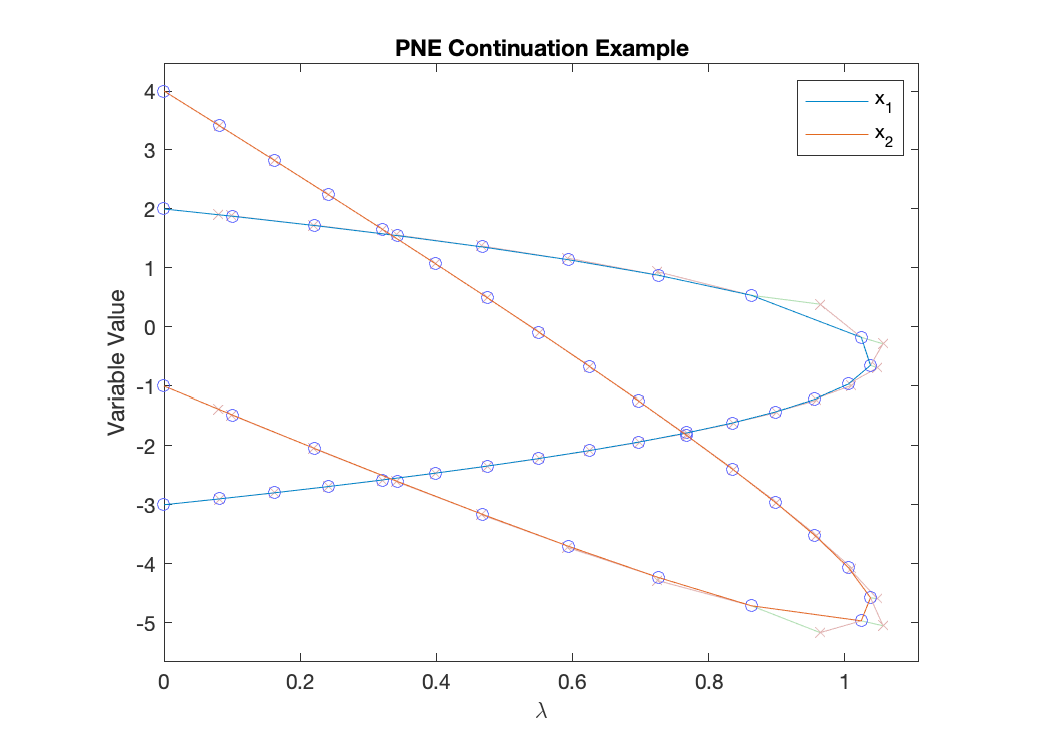
\includegraphics[width=\textwidth]{./figures/pne_ex1}
  \caption{Continuation Curve for PNE Example}
  \label{fig:pne_ex1}
\end{figure}

\begin{Code}
>> pne_ex1

MP-Opt-Model Version 4.2, 10-May-2024 -- Predictor/Corrector Continuation Method
step   0  :                          lambda =  0.000,  6 corrector steps
step   1  : PAL stepsize = 0.6       lambda =  0.081   2 corrector steps
step   2  : PAL stepsize = 0.6       lambda =  0.162   2 corrector steps
step   3  : PAL stepsize = 0.6       lambda =  0.241   2 corrector steps
step   4  : PAL stepsize = 0.6       lambda =  0.320   2 corrector steps
step   5  : PAL stepsize = 0.6       lambda =  0.398   2 corrector steps
step   6  : PAL stepsize = 0.6       lambda =  0.475   2 corrector steps
step   7  : PAL stepsize = 0.6       lambda =  0.551   2 corrector steps
step   8  : PAL stepsize = 0.6       lambda =  0.625   2 corrector steps
step   9  : PAL stepsize = 0.6       lambda =  0.697   2 corrector steps
step  10  : PAL stepsize = 0.6       lambda =  0.767   2 corrector steps
step  11  : PAL stepsize = 0.6       lambda =  0.835   2 corrector steps
step  12  : PAL stepsize = 0.6       lambda =  0.898   2 corrector steps
step  13  : PAL stepsize = 0.6       lambda =  0.956   2 corrector steps
step  14  : PAL stepsize = 0.6       lambda =  1.005   3 corrector steps
step  15  : PAL stepsize = 0.6       lambda =  1.038   3 corrector steps
step  16  : PAL stepsize = 0.6       lambda =  1.024   3 corrector steps
step  17  : PAL stepsize = 0.6       lambda =  0.863   3 corrector steps
step  18  : PAL stepsize = 0.6       lambda =  0.726   3 corrector steps
step  19  : PAL stepsize = 0.6       lambda =  0.595   3 corrector steps
step  20  : PAL stepsize = 0.6       lambda =  0.468   2 corrector steps
step  21  : PAL stepsize = 0.6       lambda =  0.343   2 corrector steps
step  22  : PAL stepsize = 0.6       lambda =  0.221   2 corrector steps
step  23  : PAL stepsize = 0.6       lambda =  0.100   2 corrector steps
step  24a : PAL stepsize = 0.6       lambda = -0.019   2 corrector steps ^ ROLLBACK
step  24  : NAT stepsize = 0.1       lambda =  0.000   3 corrector steps
CONTINUATION TERMINATION: Traced full continuation curve in 24 continuation steps

exitflag = 1
output.max_lam = 1.03783

x = 
   2
  -1
   0

f = 
            0
  -6.4837e-13

jac =
   1   1   6
  -4   1   0
\end{Code}


%%------------------------------------------
\clearpage
\section{Mathematical Model Class -- {\tt mp.opt\_model}}
\label{sec:mp_opt_model}

The \code{mp.opt\_model} class provides facilities for constructing a mathematical programming or optimization problem by adding and managing the indexing of sets of variables, constraints and costs. The model can then be solved by simply calling the \code{solve} method which automatically selects and calls the appropriate master solver function, i.e. \code{qps\_master}, \code{miqps\_master}, \code{qcqps\_master}, \code{nlps\_master}, \code{nleqs\_master} or \code{mplinsolve}, depending on the type of problem.

In this manual, and in the code, \code{mm} is the name of the variable used by convention for mathematical model objects of the class \code{mp.opt\_model}, which is typically created by calling the constructor \code{mp.opt\_model} with no arguments.\footnote{The name \code{om} is used for legacy mathematical model objects of the class \code{opt\_model}.}.

\begin{Code}
mm = mp.opt_model;
\end{Code}

Variables, constraints and costs can then be added to the model using named sets. For variables and constraints, each set represents a column vector, and the sets are stacked in the order they are added to construct the full variable vector or full constraint vector. For costs, each set represents a component of a scalar cost, and the components are summed together to construct the full objective function value.

\subsection*{Important Note}

\mpom{} 5.0 introduced a major refactorization of the mathematical model code, with the legacy mathematical model class \code{opt\_model} being replaced by the new \code{mp.opt\_model}. The legacy class, described in Appendix~\ref{app:legacy_opt_model}, provides backward compatibility with previous versions.

In both cases, the mathematical model class manages a number \emph{set types}, such as variables and several types of constraints and costs. Each set type corresponds to a particular property in the model object, and is an instance of a subclass of \code{mp.set\_manager}, as summarized in Table~\ref{tab:set_types}.

\begin{table}[!ht]
%\renewcommand{\arraystretch}{1.2}
\centering
\begin{threeparttable}
\caption{Set Types}
\label{tab:set_types}
\footnotesize
\begin{tabular}{cll}
\toprule
property name & \code{mp.set\_manager} subclass & used to manage \\
\midrule
\code{var}	& \code{mp.sm\_variable}	& variables	\\
\code{lin}	& \code{mp.sm\_lin\_constraint}	& linear constraints	\\
\code{qcn}\tnote{\dag}	& \code{mp.sm\_quad\_constraint}	& quadratic constraints	\\
\code{nle}	& \code{mp.sm\_nln\_constraint}	& nonlinear equality constraints	\\
\code{nli}	& \code{mp.sm\_nln\_constraint}	& nonlinear inequality constraints	\\
\code{qdc}	& \code{mp.sm\_quad\_cost}\tnote{\ddag}	& quadratic costs	\\
\code{nlc}	& \code{mp.sm\_nln\_cost}	& general nonlinear costs	\\
\bottomrule
\end{tabular}
\begin{tablenotes}
 \scriptsize
 \item [\dag] {While this feature is not officially supported, the quadratic cost property has also been added to the legacy \code{opt\_model} class, and works just as in \code{mp.opt\_model}.}
 \item [\ddag] {In the legacy \code{opt\_model} class, the \code{qdc} property uses the \code{mp.sm\_quad\_cost\_legacy} class for backward compatibility.}
\end{tablenotes}
\end{threeparttable}
\end{table}


\subsection{Adding Variables}
\label{sec:var_add}

\begin{Code}
mm.var.add(name, N);
mm.var.add(name, N, v0);
mm.var.add(name, N, v0, vl);
mm.var.add(name, N, v0, vl, vu);
mm.var.add(name, N, v0, vl, vu, vt);
mm.var.add(name, idx_list, N ...);
\end{Code}

A named set of variables is added to the model using the \code{add} method of the \code{var} property, where \code{name} is a string containing the name of the set\footnote{A set name must be a valid field name for a struct.}, \code{N} is the number $n$ of variables in the set, \code{v0} is the initial value of the variables, \code{vl} and \code{vu} are the upper and lower bounds on the variables, and \code{vt} is the variable type. The accepted values for \code{vt} are:
\begin{itemize}
\setlength{\parskip}{-6pt}%
\item \codeq{C} – continuous
\item \codeq{I} – integer
\item \codeq{B} – binary, i.e. 0 or 1
\end{itemize}
The inputs \code{v0}, \code{vl} and \code{vu} are $n \times 1$ column vectors, \code{vt} is a scalar or a $1 \times n$ row vector. The defaults for the last four arguments, which are all optional, are for all to be continuous, unbounded and initialized to zero. That is, \code{v0}, \code{vl}, \code{vu}, and \code{vt} default to 0, $-\infty$, $+\infty$, and \codeq{C}, respectively.

For example, suppose our problem has variables $u$, $v$ and $w$, which are vectors of length $n_u$, $n_v$, and $n_w$, respectively, where $u$ is unbounded, $v$ is non-negative and the lower and upper bounds on $w$ are given in the vectors \code{wlb} and \code{wub}. Let us further suppose that the initial value of $w$ is provided in \code{w0} and the first 3 elements of $w$ are binary variables. And we will assume that the values of $n_u$, $n_v$, and $n_w$ are available in the variables \code{nu}, \code{nv} and \code{nw}, respectively.

We can then add these variable sets to the model with the names \textbf{u}, \textbf{v}, and \textbf{w}, as follows:
\begin{Code}
wtype = repmat('C', 1, nw);  wt(1:3) = 'B';
mm.var.add('u', nu);
mm.var.add('v', nv, [], 0);
mm.var.add('w', nw, w0, wlb, wub, wtype);
\end{Code}
In this case, then, the full variable vector is the $(n_u+n_v+n_w) \times 1$ vector
\begin{equation}
x = \left[\begin{array}{c}u \\ v \\ w \end{array}\right]. \label{eq:x}
\end{equation}

See Section~\ref{sec:indexed_sets} for details on indexed named sets and the \code{idx\_list} argument.

\subsubsection{Variable Subsets}
\label{sec:varsets}

A key feature of \mpom{} is that each set of constraints or costs can be defined in terms of the relevant variables only, as opposed to the entire vector~$x$. This is done by specifying a variable subset, a cell array of the variable names of interest, in the \code{varsets} argument. Besides simplifying the constraint and cost definitions, another benefit of this approach is that it allows a model to be modified with new variables after some constraints and costs have already been added.

In the sections to follow, we will use the following two variable subsets for illustration purposes:
\begin{itemize}
\setlength{\parskip}{-6pt}%
\item \code{\{}\codeq{v}\code{\}} corresponding to $x_1 \equiv v$, and
\item \code{\{}\codeq{u}\code{, }\codeq{w}\code{\}} corresponding to $x_2 \equiv \left[\begin{array}{c}u \\ w \end{array}\right]$.
\end{itemize}

\subsection{Adding Constraints}
\label{sec:constraint}

A named set of constraints can be added to the model as soon as the variables on which it depends have been added. \mpom{} currently supports four types of constraints, doubly-bounded linear constraints, doubly-bounded quadratic constraints, general nonlinear equality constraints, and general nonlinear inequality constraints.

\subsubsection{Linear Constraints}
\label{sec:lin_add}

\begin{Code}
mm.lin.add(mm.var, name, A, l, u);
mm.lin.add(mm.var, name, A, l, u, varsets);
mm.lin.add(mm.var, name, idx_list, A ...);
\end{Code}

In \mpom{}, linear constraints take the form
\begin{equation}
l \le A x \le u,    \label{eq:linear_constraints}
\end{equation}
where $x$ here refers to either the full variable vector \emph{(default)}, or the vector obtained by stacking the subset of variables specified in \code{varsets}. Here \code{A} contains the $n_A \times n_x$ matrix $A$ and \code{l} and \code{u} are the $n_A \times 1$ vectors $l$ and $u$.\footnote{The \code{A} matrix can be sparse.}

For example, suppose our problem has the following three sets of linear constraints,
\begin{align}
l_1 \le &A_1 x_1 \le u_1 \\
l_2 \le &A_2 x_2 \\
&A_3 x \le u_3,
\end{align}
where $x_1$ and $x_2$ are as defined in Section~\ref{sec:varsets} and $x$ is the full variable vector from \eqref{eq:x}. Notice that the number of columns in $A_1$ and $A_2$ correspond to $n_v$ and $n_u+n_w$, respectively, whereas $A_3$ has the full set of columns corresponding to $x$.

These three linear constraint sets can be added to the model with the names \textbf{lincon1}, \textbf{lincon2}, and \textbf{lincon3}, using the \code{add} method of the \code{lin} property as follows:
\begin{Code}
mm.lin.add(mm.var, 'lincon1', A1, l1, u1, {'v'});
mm.lin.add(mm.var, 'lincon2', A2, l2, [], {'u', 'w'});
mm.lin.add(mm.var, 'lincon3', A3, [], u3);
\end{Code}

See Section~\ref{sec:indexed_sets} for details on indexed named sets and the \code{idx\_list} argument.

\subsubsection{Quadratic Constraints}
\label{sec:qcn_add}

\begin{Code}
mm.qdc.add(mm.var, name, Q, B, l, u);
mm.qdc.add(mm.var, name, Q, B, l, u, varsets);
mm.qdc.add(mm.var, name, idx_list, Q, ...);
\end{Code}

In \mpom{}, quadratic constraints take the form
\begin{equation}
\llqi \le \frac{1}{2} \trans{x} Q_i x + b_i x \le \uuqi, \quad \forall i = 1, \dots, n_q \label{eq:quadratic_constraints}
\end{equation}
where $x$ here refers to either the full variable vector \emph{(default)}, or the vector obtained by stacking the subset of variables specified in \code{varsets}. Here \code{Q} is an $n_q \times 1$ cell array of the $n_x \times n_x$ matrices $Q_i$, \code{B} contains the $n_q \times n_x$ matrix $B$, of which $b_i$ is row~$i$, and \code{l} and \code{u} are the $n_q \times 1$ vectors $\llq$ and $\uuq$.\footnote{The matrices in \code{Q} and \code{B} can be sparse.}

For example, suppose our problem has the following three sets of quadratic constraints,
\begin{align}
l_1 \le & \left[ \begin{array}{c} \trans{x_1} Q_{11} x_1 + b_{11} x_1 \\ 
       \trans{x_1} Q_{12} x_1 + b_{12} x_1 \end{array} \right] \le u_1 \\
l_2 \le &\trans{x_2} Q_2 x_2 + b_2 x_2 \\
&\trans{x} Q_3 x + b_3 x \le u_3,
\end{align}
where $x_1$ and $x_2$ are as defined in Section~\ref{sec:varsets} and $x$ is the full variable vector from \eqref{eq:x}. Notice that the number of columns in $Q_{11}$, $Q_{12}$, $b_{11}$, and $b_{12}$ correspond to $n_v$ and for $Q_2$ and $b_2$ to $n_u+n_w$. On the other hand, $Q_3$ and $b_3$ have the full set of columns corresponding to $x$.

These three quadratic constraint sets can be added to the model with the names \textbf{quadcon1}, \textbf{quadcon2}, and \textbf{quadcon3}, using the \code{mm.qcn.add} method as follows:
\begin{Code}
Q1 = {Q11; Q12}; B1 = [b11; b12];
mm.qcn.add(mm.var, 'quadcon1', Q1, B1, l1, u1, {'v'});
mm.qcn.add(mm.var, 'quadcon2', {Q2}, b2, l2, [], {'u', 'w'});
mm.qcn.add(mm.var, 'quadcon3', {Q3}, b3, [], u3);
\end{Code}

See Section~\ref{sec:indexed_sets} for details on indexed named sets and the \code{idx\_list} argument.

\subsubsection{General Nonlinear Constraints}
\label{sec:nlx_add}

\emph{Equality Constraints}
\begin{Code}
mm.nle.add(mm.var, name, N, fcn, hess);
mm.nle.add(mm.var, name, N, fcn, hess, varsets);
mm.nle.add(mm.var, name, idx_list, N ...);
\end{Code}
\emph{Inequality Constraints}
\begin{Code}
mm.nli.add(mm.var, name, N, fcn, hess);
mm.nli.add(mm.var, name, N, fcn, hess, varsets);
mm.nli.add(mm.var, name, idx_list, N ...);
\end{Code}

\mpom{} allows the user to implement general nonlinear constraints of the form
\begin{align}
g(x) &= 0, \textrm{~or} \\
g(x) &\le 0
\end{align}
by providing the handle \code{fcn} of a function that evaluates the constraint and its Jacobian and another handle \code{hess} of a function that evaluates the Hessian. The number of constraints in the set is given by \code{N}, and the \code{nle} property is used for an equality constraint or the \code{nli} property for an inequality.

The calling syntax for \code{fcn} is:
\begin{Code}
g = fcn(x);
[g, dg] = fcn(x);
\end{Code}
Here \code{g} is the $n_g \times 1$ vector $g(x)$ and \code{dg} is the $n_g \times n_x$ Jacobian matrix $J(x)$, where $J_{ij} = \der{g_i}{x_j}$.

Rather than computing the full three-dimensional Hessian, the \code{hess} function actually evaluates the Jacobian of the vector $\trans{J}(x) \lambda$ for a specified value of the vector $\lambda$. The calling syntax for \code{hess} is:
\begin{Code}
d2g = hess(x, lambda);
\end{Code}

For both functions, the first input argument \code{x} takes one of two forms. If the constraint set is added with \code{varsets} empty or missing, then \code{x} will be the full variable vector. Otherwise it will be a cell array of vectors corresponding to the variable sets specified in \code{varsets}.

There is also the option for \code{name} to be a cell array of constraint set names, in which case \code{N} is a vector, specifying the number of constraints in each corresponding set. In this case, \code{fcn} and \code{hess} are each still a single function handle, but the values computed by each correspond to the entire stacked collection of constraint sets together, as if they were a
single set.

For example, suppose our problem has the following three sets of nonlinear constraints,
\begin{align}
g_1(x_1) \le 0 \\
g_2(x_2) = 0 \\
g_3(x) \le 0,
\end{align}
where $x_1$ and $x_2$ are as defined in Section~\ref{sec:varsets} and $x$ is the full variable vector from \eqref{eq:x}. Let \code{my\_cons\_fcn1}, \code{my\_cons\_fcn2}, and \code{my\_cons\_fcn3} be functions that evaluate $g_1(x_1)$, $g_2(x_2)$, and $g_3(x)$ and their gradients, respectively. Similarly, let \code{my\_cons\_hess1}, \code{my\_cons\_hess2}, and \code{my\_cons\_hess3} be Hessian evaluation functions for the same. The variables \code{ng1}, \code{ng2}, and \code{ng3} contain the number of constraints in the respective constraint sets.

These three nonlinear constraint sets can be added to the model with the names \textbf{nlncon1}, \textbf{nlncon2}, and \textbf{nlncon3}, using the \code{add} method of the \code{nle} and \code{nli} properties as follows:
\begin{Code}
fcn1 = @(x)my_cons_fcn1(x, <other_args>);
fcn2 = @(x)my_cons_fcn2(x, <other_args>);
fcn3 = @(x)my_cons_fcn3(x, <other_args>);
hess1 = @(x, lambda)my_cons_hess1(x, lambda, <other_args>);
hess2 = @(x, lambda)my_cons_hess2(x, lambda, <other_args>);
hess3 = @(x, lambda)my_cons_hess3(x, lambda, <other_args>);
mm.nli.add(mm.var, 'nlncon1', ng1, 0, fcn1, hess1 {'v'});
mm.nle.add(mm.var, 'nlncon2', ng2, 1, fcn2, hess2, {'u', 'w'});
mm.nli.add(mm.var, 'nlncon3', ng3, 0, fcn3, hess3);
\end{Code}
In this case, the \code{x} variable passed to the \code{my\_cons\_fcn} and \code{my\_cons\_hess} functions will be as follows:
\begin{itemize}
\setlength{\parskip}{-6pt}%
\item \code{my\_cons\_fcn1}, \code{my\_cons\_hess1} $\longrightarrow$ \code{x} = \code{\{}$v$\code{\}}
\item \code{my\_cons\_fcn2}, \code{my\_cons\_hess2} $\longrightarrow$ \code{x} = \code{\{}$u, w$\code{\}}
\item \code{my\_cons\_fcn3}, \code{my\_cons\_hess3} $\longrightarrow$ \code{x} = \code{[}$u; v; w$\code{]}
\end{itemize}

See Section~\ref{sec:indexed_sets} for details on indexed named sets and the \code{idx\_list} argument.

\subsection{Adding Costs}
\label{sec:cost}

The objective of an \mpom{} optimization problem is to \emph{minimize} the sum of all costs added to the model. As with constraints, a named set of costs can be added to the model as soon as the variables on which it depends have been added. \mpom{} currently supports two types of costs, quadratic costs and general nonlinear costs.

\subsubsection{Quadratic Costs}
\label{sec:qdc_add}

\begin{Code}
mm.qdc.add(mm.var, name, H, c);
mm.qdc.add(mm.var, name, H, c, k);
mm.qdc.add(mm.var, name, H, c, k, varsets);
mm.qdc.add(mm.var, name, idx_list, H ...);
\end{Code}

A quadratic cost set takes the form:
\begin{equation}
f(x) = \frac{1}{2} \trans{x} H x + \trans{c} x + k \label{eq:quad_cost}
\end{equation}
where $x$ here refers to either the full variable vector \emph{(default)}, or the vector obtained by stacking the subset of variables specified in \code{varsets}. Here \code{H} contains the $n_x \times n_x$ matrix $H$, \code{c} the $n_x \times 1$ vector $c$, and \code{k} the scalar $k$.\footnote{The \code{H} matrix can be sparse.}

Alternatively, if \code{H} is an $n_x \times 1$ vector, then $f(x)$ is also an $n_x \times 1$ vector, \code{k} can be $n_x \times 1$ or scalar, and the $i$-th element of $f(x)$ is given by
\begin{equation}
f_i(x) = \frac{1}{2} H_i x_i^2 + c_i x_i + k_i. \label{eq:quad_cost2}
\end{equation}
where $k_i = $~\code{k} for all $i$ if \code{k} is scalar. If \code{H} is empty, then form \eqref{eq:quad_cost} is implied by a scalar \code{k} and \eqref{eq:quad_cost2} by a vector \code{k}.

For example, suppose our problem has the following three sets of quadratic costs,
\begin{align}
q_1(x_1) &= \frac{1}{2} \trans{x_1} H_1 x_1 + \trans{c_1} x_1 + k_1 \\
q_2(x_2) &= \frac{1}{2} \trans{x_2} H_2 x_2 + \trans{c_2} x_2 + k_2 \\
q_3(x) &= \frac{1}{2} \trans{x} H_3 x + \trans{c_3} x + k_3,
\end{align}
where $x_1$ and $x_2$ are as defined in Section~\ref{sec:varsets} and $x$ is the full variable vector from \eqref{eq:x}. Notice that the dimensions of $H_1$ and $H_2$ (and $c_1$ and $c_2$) correspond to $n_v$ and $n_u+n_w$, respectively, whereas $H_3$ (and $c_3$) correspond to the full $x$.

These three quadratic cost sets can be added to the model with the names \textbf{qcost1}, \textbf{qcost2}, and \textbf{qcost3}, using the \code{add\_quad\_cost} method as follows:
\begin{Code}
mm.qdc.add(mm.var, 'qcost1', H1, c1, k1, {'v'});
mm.qdc.add(mm.var, 'qcost2', H2, c2, k2, {'u', 'w'});
mm.qdc.add(mm.var, 'qcost3', H3, c3, k3);
\end{Code}

See Section~\ref{sec:indexed_sets} for details on indexed named sets and the \code{idx\_list} argument.

\subsubsection{General Nonlinear Costs}
\label{sec:nlc.add}

\begin{Code}
mm.nlc.add(mm.var, name, N, fcn);
mm.nlc.add(mm.var, name, N, fcn, varsets);
mm.nlc.add(mm.var, name, idx_list, N ...);
\end{Code}

\mpom{} allows the user to implement a general nonlinear cost by providing the handle \code{fcn} of a function that evaluates the cost $f(x)$, its gradient and Hessian $H$, as described below. The \code{N} parameter specifies the dimension for vector valued cost functions, which are not yet implemented. Currently \code{N} must equal 1 or it will throw an error.

For a cost function $f(x)$, \code{fcn} should point to a function with the
following interface:
\begin{Code}
f = fcn(x)
[f, df] = fcn(x)
[f, df, d2f] = fcn(x)
\end{Code}
where \code{f} is a scalar with the value of the function $f(x)$, \code{df} is the $n_x \times 1$ gradient of $f$, and \code{d2f} is the $n_x \times n_x$ Hessian $H$, where $n_x$ is the number of elements in $x$.

The first input argument \code{x} takes one of two forms. If the constraint set is added with \code{varsets} empty or missing, then \code{x} will be the full variable vector. Otherwise it will be a cell array of vectors corresponding to the variable sets specified in \code{varsets}.

For example, suppose our problem has three sets of nonlinear costs, $f_1(x_1)$, $f_2(x_2)$, $f_3(x)$, where $x_1$ and $x_2$ are as defined in Section~\ref{sec:varsets} and $x$ is the full variable vector from \eqref{eq:x}. Let \code{my\_cost\_fcn1}, \code{my\_cost\_fcn2}, and \code{my\_cost\_fcn3} functions that evaluate $f_1(x)$, $f_2(x)$, and $f_3(x)$ and their gradients and Hessians, respectively.

These three nonlinear cost sets can be added to the model with the names \textbf{nlncost1}, \textbf{nlncost2}, and \textbf{nlncost3}, using the \code{add} method of the \code{nlc} property as follows:
\begin{Code}
fcn1 = @(x)my_cost_fcn1(x, <other_args>);
fcn2 = @(x)my_cost_fcn2(x, <other_args>);
fcn3 = @(x)my_cost_fcn3(x, <other_args>);
mm.nlc.add(mm.var, 'nlncost1', 1, fcn1 {'v'});
mm.nlc.add(mm.var, 'nlncost2', 1, fcn2, {'u', 'w'});
mm.nlc.add(mm.var, 'nlncost3', 1, fcn3);
\end{Code}
In this case, the \code{x} variable passed to the \code{my\_cost\_fcn} functions will be as follows:
\begin{itemize}
\setlength{\parskip}{-6pt}%
\item \code{my\_cost\_fcn1} $\longrightarrow$ \code{x} = \code{\{}$v$\code{\}}
\item \code{my\_cost\_fcn2} $\longrightarrow$ \code{x} = \code{\{}$u, w$\code{\}}
\item \code{my\_cost\_fcn3} $\longrightarrow$ \code{x} = \code{[}$u; v; w$\code{]}
\end{itemize}

See Section~\ref{sec:indexed_sets} for details on indexed named sets and the \code{idx\_list} argument.

\clearpage
\subsection{Solving the Model}
\label{sec:solve}

\begin{Code}
mm.solve()
[x, f, exitflag, output, jac] = mm.solve()
[x, f, exitflag, output, lambda] = mm.solve(opt)
[...] = mm.solve(opt)
\end{Code}

After all variables, constraints and costs have been added to the model, the mathematical programming or optimization problem can be solved simply by calling the \code{solve} method. This method automatically selects and calls, depending on the problem type, \code{mplinsolve} or one of the master solver interface functions from Section~\ref{sec:master_solvers}, namely \code{qps\_master}, \code{miqps\_master}, \code{qcqps\_master}, \code{nlps\_master}, \code{nleqs\_master}, or \code{pnes\_master}. Note that one of the equation solvers is chosen if the model has no costs and no inequality constraints. In this case, if the number of variables is equal to the number of equality constraints, \code{mplinsolve} or \code{nleqs\_master} is selected. If the number of variables is one more than the number of constraints \code{pnes\_master} is chosen.

The results are stored in the \code{soln} field (see Section~\ref{sec:soln}) of the \mpom{} object and can be returned in the optional output arguments. The input options struct \code{opt}, summarized in Tables~\ref{tab:solve_options} and \ref{tab:solve_alg_option}, is optional, as are all of its fields. For details on the return values see the descriptions of the individual solver functions in Sections~\ref{sec:qps_master}, \ref{sec:miqps_master}, \ref{sec:qcqps_master}, \ref{sec:nlps_master}, \ref{sec:nleqs_master}, and \ref{sec:pnes_master}. For linear equations, the \code{solver} and \code{opt} arguments for \code{mplinsolve}, described in Section~\ref{MIPSMAN-sec:mplinsolve} of the \mipsman{}, can be provided in the respective fields of \code{opt.leq\_opt}.


\begin{table}[!ht]
%\renewcommand{\arraystretch}{1.2}
\centering
\begin{threeparttable}
\caption{Options for \code{solve}}
\label{tab:solve_options}
\footnotesize
\begin{tabular}{lcp{0.62\textwidth}}
\toprule
name & default & description \\
\midrule
% \multicolumn{3}{l}{\emph{General Options}} \\
\code{~~alg}	& \codeq{DEFAULT}	& determines which solver to use, see Table~\ref{tab:solve_alg_option} \\
\code{~~verbose}	& 1	& amount of progress info to be printed \\
&& \begin{tabular}{r @{ -- } l}
0 & print no progress info \\
1--5 & print increasing level of progress info \\
\end{tabular}	\\
\code{~~parse\_soln}	& 0	& flag that specifies whether or not to call the \code{parse\_soln} method and place the return values in the \code{soln}
property of the field type objects \\
\code{~~relax\_integer}	& 0	& relax integer constraints, if true \\
\code{~~x0}	& \emph{empty}	& optional initial value of $x$, overrides value stored in model, \emph{(ignored by some solvers)}	\\
\midrule
\multicolumn{3}{l}{\emph{Additional Options for Specific Problem Types}} \\
% \emph{problem type} & & \emph{for details see ...} \\
~~LP/QP & & see Table~\ref{tab:qps_master_options} \\
~~MILP/MIQP & & see Table~\ref{tab:miqps_master_options} \\
~~QCQP & & see Table~\ref{tab:qcqps_master_options} \\
~~NLP & & see Table~\ref{tab:nlps_master_options} \\
~~LEQ & & see Section~\ref{MIPSMAN-sec:mplinsolve} of the \mipsman{} \\
~~~~\code{leq\_opt.solver} & \codeq{} & see \code{help mplinsolve}, input argument \code{solver} \\
~~~~\code{leq\_opt.opt} & \emph{empty} & see \code{help mplinsolve}, input argument \code{opt} \\
~~NLEQ & & see Table~\ref{tab:nleqs_master_options} \\
~~PNE & & see Table~\ref{tab:pnes_master_options} \\
\bottomrule
\end{tabular}
% \begin{tablenotes}
%  \scriptsize
%  \item [*] {}
% \end{tablenotes}
\end{threeparttable}
\end{table}

\clearpage

\begin{table}[!ht]
%\renewcommand{\arraystretch}{1.2}
\centering
\begin{threeparttable}
\caption{Values for \code{alg} Option to \code{solve}}
\label{tab:solve_alg_option}
\footnotesize
\begin{tabular}{lcp{0.55\textwidth}}
\toprule
\code{alg} value & problem type(s) & description \\
\midrule
\codeq{DEFAULT} & \emph{all} & automatic, depends on problem type, uses first available of: \\
& LP & \gurobi{}, \cplex{}, \mosek{}, \code{linprog}\tnote{\P}, \highs{}, \glpk{}, BPMPD, \mips{} \\
& QP & \gurobi{}, \cplex{}, \mosek{}, \code{quadprog}\tnote{\P}, \highs{}, BPMPD, \mips{} \\
& MILP & \gurobi{}, \cplex{}, \mosek{}, \code{intlinprog}, \highs{}, \glpk{} \\
& MIQP & \gurobi{}, \cplex{}, \mosek{} \\
& QCQP & \ipopt{}, \knitro{}, \code{fmincon}\tnote{\P}, \mips{} \\
& NLP & \mips{} \\
& MINLP & \knitro{} (not yet implemented) \\
& LEQ & built-in backslash operator \\
& NLEQ & Newton's method \\
& PNE & predictor/corrector continuation method \\
\codeq{BPMPD} & LP, QP & BPMPD\tnote{*} \\
\codeq{CLP} & LP, QP & \clp{}\tnote{*} \\
\codeq{CPLEX} & LP, QP, MILP, MIQP & \cplex{}\tnote{*} \\
\codeq{FD} & NLEQ & fast-decoupled Newton's method\tnote{\dag} \\
\codeq{FMINCON} & QCQP, NLP & \matlab{} Opt Toolbox, \code{fmincon}\tnote{*} \\
\codeq{FSOLVE} & NLEQ & \matlab{} Opt Toolbox, \code{fsolve}\tnote{\S} \\
\codeq{GLPK} & LP, MILP & \glpk{}\tnote{*} \emph{(LP only)} \\
\codeq{GS} & NLEQ & Gauss-Seidel method\tnote{\ddag} \\
\codeq{GUROBI} & LP, QP, MILP, MIQP, QCQP & \gurobi{}\tnote{*} \\
\codeq{HIGHS} & LP, QP, MILP & \highs{}\tnote{*} \\
\codeq{IPOPT} & LP, QP, QCQP, NLP & \ipopt{}\tnote{*} \\
\codeq{KNITRO} & QCQP, NLP, MINLP & \knitro{}\tnote{*} \\
\codeq{MIPS} & LP, QP, QCQP, NLP & \mipslink{}, \mipsname{} \\
\codeq{MOSEK} & LP, QP, MILP, MIQP & \mosek{}\tnote{*} \\
\codeq{NEWTON} & NLEQ & Newton's method \\
\codeq{OSQP} & LP, QP & \osqp{}\tnote{*} \\
\codeq{OT} & LP, QP, MILP & \matlab{} Opt Toolbox, \code{quadprog}, \code{linprog}, \code{intlinprog} \\
\bottomrule
\end{tabular}
\begin{tablenotes}
 \scriptsize
 \item [*] {Requires the installation of an optional package. See Appendix~\ref{app:optional_packages} for details on the corresponding package.}
 \item [\dag] {Fast-decoupled Newton requires setting \code{fd\_opt.jac\_approx\_fcn} to a function handle that returns Jacobian approximations. See \code{help nleqs\_fd\_newton} for more details.}
 \item [\ddag] {Gauss-Seidel requires setting \code{gs\_opt.x\_update\_fcn} to a function handle that updates $x$. See \code{help nleqs\_gauss\_seidel} for more details.}
 \item [\S] {The \code{fsolve} function is included with GNU Octave, but on \matlab{} it is part of the \matlab{} \ot{}. See Appendix~\ref{app:optional_packages} for more information on the \matlab{} \ot{}.}
 \item [\P] {If running on \matlab{}.}
\end{tablenotes}
\end{threeparttable}
\end{table}


\subsection{Accessing the Model}

\subsubsection{Indexing}

For each set type, \mpom{} maintains indexing information\footnote{This indexing information is managed by the \code{mp.set\_manager} base class from which all set type objects inherit.} for each named set that is added, including the number of elements and the starting and ending indices. This information is stored in the \code{idx} property of the set type object, consisting of a struct with fields \code{N}, \code{i1}, and \code{iN}, for storing number of elements, starting index and ending index, respectively. Each of these fields is also a struct with field names corresponding to the named sets.

For example, if we have added the \textbf{u}, \textbf{v}, and \textbf{w} variables as in Section~\ref{sec:var_add}, then the contents of \code{mm.var.idx} will be as shown in Table~\ref{tab:vv}.

\begin{table}[!ht]
%\renewcommand{\arraystretch}{1.2}
\centering
\begin{threeparttable}
\caption{Example Indexing Data}
\label{tab:vv}
\footnotesize
\begin{tabular}{lcl}
\toprule
field & value & description \\
\midrule
% \code{vv}	& 	& indexing information for all variables \\
% \code{~~.N}	& 	& number of elements for each variable \\
% \code{~~~~.u}	& $n_u$	& number of $u$ variables \\
% \code{~~~~.v}	& $n_v$	& number of $v$ variables \\
% \code{~~~~.w}	& $n_w$	& number of $w$ variables \\
% \code{~~.i1}	& 	& starting index in $x$ for each variable \\
% \code{~~~~.u}	& 1	& starting index of $u$ in full $x$ \\
% \code{~~~~.v}	& $n_u + 1$	& starting index of $v$ in full $x$ \\
% \code{~~~~.w}	& $n_u + n_v + 1$	& starting index of $w$ in full $x$ \\
% \code{~~.iN}	& 	& ending index in $x$ for each variable \\
% \code{~~~~.u}	& $n_u$	& ending index of $u$ in full $x$ \\
% \code{~~~~.v}	& $n_u + n_v$	& ending index of $v$ in full $x$ \\
% \code{~~~~.w}	& $n_u + n_v + n_w$	& ending index of $w$ in full $x$ \\
% \\
\code{mm.var.idx.N.u}	& $n_u$	& number of $u$ variables \\
\code{mm.var.idx.N.v}	& $n_v$	& number of $v$ variables \\
\code{mm.var.idx.N.w}	& $n_w$	& number of $w$ variables \\
\code{mm.var.idx.i1.u}	& 1	& starting index of $u$ in full $x$ \\
\code{mm.var.idx.i1.v}	& $n_u + 1$	& starting index of $v$ in full $x$ \\
\code{mm.var.idx.i1.w}	& $n_u + n_v + 1$	& starting index of $w$ in full $x$ \\
\code{mm.var.idx.iN.u}	& $n_u$	& ending index of $u$ in full $x$ \\
\code{mm.var.idx.iN.v}	& $n_u + n_v$	& ending index of $v$ in full $x$ \\
\code{mm.var.idx.iN.w}	& $n_u + n_v + n_w$	& ending index of $w$ in full $x$ \\
\bottomrule
\end{tabular}
\end{threeparttable}
\end{table}

\subsubsection*{\code{get\_idx}}
\label{sec:get_idx}
\begin{Code}
[idx1, idx2, ...] = mm.get_idx(set_type1, set_type2, ...);
vv = mm.get_idx('var');
[ll, nne, nni] = mm.get_idx('lin', 'nle', 'nli');

vv = mm.get_idx()
[vv, ll] = mm.get_idx()
[vv, ll, nne] = mm.get_idx()
[vv, ll, nne, nni] = mm.get_idx()
[vv, ll, nne, nni, qq] = mm.get_idx()
[vv, ll, nne, nni, qq, nnc] = mm.get_idx()
[vv, ll, nne, nni, qq, nnc, qqcn] = mm.get_idx()
\end{Code}

The \code{idx} property of indexing information for each set type is available via the \code{get\_idx} method of \code{mp.opt\_model}. When called with one or more set type property names as inputs, it returns the corresponding indexing structs. The list of valid set type strings is shown in Table~\ref{tab:valid_set_types}. When called without input arguments, the indexing structs are simply returned in the order listed in the table.

\begin{table}[!ht]
%\renewcommand{\arraystretch}{1.2}
\centering
\begin{threeparttable}
\caption{Valid Set Types}
\label{tab:valid_set_types}
\footnotesize
\begin{tabular}{ccl}
\toprule
set type string & var name\tnote{*} & description \\
\midrule
\codeq{var}	& \code{vv}	& variables	\\
\codeq{lin}	& \code{ll}	& linear constraints	\\
\codeq{qcn}	& \code{qqcn}	& quadratic constraints	\\
\codeq{nle}	& \code{nne}	& nonlinear equality constraints	\\
\codeq{nli}	& \code{nni}	& nonlinear inequality constraints	\\
\codeq{qdc}	& \code{qq}	& quadratic costs	\\
\codeq{nlc}	& \code{nnc}	& general nonlinear costs	\\
\bottomrule
\end{tabular}
\begin{tablenotes}
 \scriptsize
 \item [*] {The name of the variable used by convention for this indexing struct.}
\end{tablenotes}
\end{threeparttable}
\end{table}

For the example model built in Sections~\ref{sec:var_add}--\ref{sec:cost}, where \code{x} and \code{lambda} are return values from the \code{solve} method, we can, for example, access the solved value of $v$ and the shadow prices on the \textbf{nlncon3} constraints with the following code.
\begin{Code}
[vv, nne] = mm.get_idx('var', 'nle');
v = x(vv.i1.v:vv.iN.v);
lam_nln3 = lambda.ineqnonlin(nni.i1.nlncon3:nni.iN.nlncon3);
\end{Code}


\subsubsection{Variables}

\subsubsection*{\code{var.params}}
\label{sec:var_params}
\begin{Code}
[v0, vl, vu] = mm.var.params()
[v0, vl, vu] = mm.var.params(name)
[v0, vl, vu] = mm.var.params(name, idx_list)
[v0, vl, vu, vt] = mm.var.params(...)
\end{Code}

The \code{params} method of the \code{var} property returns the initial value \code{v0}, lower bound \code{vl} and upper bound \code{vu} for the full variable vector $x$, or for a specific named variable set. Optionally also returns a corresponding char vector \code{vt} of variable types, where \codeq{C}, \codeq{I} and \codeq{B} represent continuous, integer, and binary variables, respectively.

\noindent \\Examples:
\begin{Code}
[x0, xmin, xmax] = mm.var.params();
[w0, wlb, wub, wtype] = mm.var.params('w');
\end{Code}

See Section~\ref{sec:indexed_sets} for details on indexed named sets and the \code{idx\_list} argument.

\subsubsection{Constraints}

\subsubsection*{\code{lin.params}}
\begin{Code}
[A, l, u] = mm.lin.params(mm.var)
[A, l, u] = mm.lin.params(mm.var, name)
[A, l, u] = mm.lin.params(mm.var, name, idx_list)
[A, l, u, vs] = mm.lin.params(mm.var, ...)
[A, l, u, vs, i1, in] = mm.lin.params(mm.var, ...)
\end{Code}

With only the \code{mm.var} input paramter, the \code{params} method of the \code{lin} property assembles and returns the parameters for the aggregate linear constraints from all linear constraint sets added using \code{mm.lin.add}. The values of these parameters are cached for subsequent calls. The parameters are $A$, $l$, and $u$, where the linear constraint is of the form
\begin{equation}
l \le A x \le u.
\end{equation}

If a \code{name} is provided then it simply returns the parameters for the corresponding named set. An optional 4th output argument \code{vs} indicates the variable sets used by this constraint set. The size of \code{A} will be consistent with \code{vs}. Optional 5th and 6th output arguments \code{i1} and \code{iN} indicate the starting and ending row indices of the corresponding constraint set in the full aggregate constraint matrix.

\noindent \\Examples:
\begin{Code}
[A, l, u] = mm.lin.params(mm.var);
[A, l, u, vs, i1, iN] = mm.lin.params(mm.var, 'lincon2');
\end{Code}

See Section~\ref{sec:indexed_sets} for details on indexed named sets and the \code{idx\_list} argument.

\subsubsection*{\code{qcn.params}}
See the reference documentation for the \code{params} method of \code{mp.sm\_quad\_constraint}.

\subsubsection*{\code{nle.params}, \code{nli.params}}

\emph{Equality Constraints}
\begin{Code}
N = mm.nle.params(mm.var, name)
N = mm.nle.params(mm.var, name, idx_list)
[N, fcn] = mm.nle.params(...)
[N, fcn, hess] = mm.nle.params(...)
[N, fcn, hess, vs] = mm.nle.params(...)
[N, fcn, hess, vs, include] = mm.nle.params(...)
\end{Code}
\emph{Inequality Constraints}
\begin{Code}
N = mm.nli.params(mm.var, name)
N = mm.nli.params(mm.var, name, idx_list)
[N, fcn] = mm.nli.params(...)
[N, fcn, hess] = mm.nli.params(...)
[N, fcn, hess, vs] = mm.nli.params(...)
[N, fcn, hess, vs, include] = mm.nli.params(...)
\end{Code}

Returns the parameters \code{N}, and optionally \code{fcn}, and \code{hess} provided when the corresponding named nonlinear constraint set was added to the model. Likewise for indexed named sets specified by \code{name} and \code{idx\_list}.

An optional 4th output argument \code{vs} indicates the variable sets used by this constraint set.

And, for constraint sets whose functions compute the constraints for another set, an optional 5th output argument returns a struct with a cell array of set names in the \codeq{name} field and an array of corresponding dimensions in the \codeq{N} field.

\subsubsection*{\code{lin.eval}}
\label{sec:lin_eval}
\begin{Code}
Ax_u = mm.lin.eval(mm.var, x)
Ax_u = mm.lin.eval(mm.var, x, name)
Ax_u = mm.lin.eval(mm.var, x, name, idx_list)
[Ax_u, l_Ax] = mm.lin.eval(...)
[Ax_u, l_Ax, A] = mm.lin.eval(...)
\end{Code}
Builds and evaluates the linear constraints $Ax - u$ and, optionally $l - Ax$ for the full set of constraints or an individual named subset for a given value of the variable vector $x$, based on constraints added by \code{mm.lin.add}.

\noindent \\Examples:
\begin{Code}
[Ax_u, l_Ax, A] = mm.lin.eval(mm.var, x);
\end{Code}

\subsubsection*{\code{qcn.eval}}
See the reference documentation for the \code{eval} method of \code{mp.sm\_quad\_constraint}.

\subsubsection*{\code{nle.eval}, \code{nli.eval}}
\label{sec:nln_eval}
\emph{Equality Constraints}
\begin{Code}
g = mm.nle.eval(mm.var, x)
g = mm.nle.eval(mm.var, x, name)
g = mm.nle.eval(mm.var, x, name, idx_list)
[g, dg] = mm.nle.eval(...)
\end{Code}
\emph{Inequality Constraints}
\begin{Code}
g = mm.nli.eval(mm.var, x)
g = mm.nli.eval(mm.var, x, name)
g = mm.nli.eval(mm.var, x, name, idx_list)
[g, dg] = mm.nli.eval(...)
\end{Code}

Builds the nonlinear equality constraints $g(x)$ or inequality constraints $h(x)$ and optionally their gradients for the full set of constraints or an individual named subset for a given value of the variable vector $x$, based on constraints added by \code{mm.nle.add} or \code{mm.nli.add}, where $g(x) = 0$ and $h(x) \le 0$.

\noindent \\Examples:
\begin{Code}
[g, dg] = mm.nle.eval(mm.var, x);
[h, dh] = mm.nli.eval(mm.var, x);
\end{Code}

\subsubsection*{\code{nle.eval\_hess}, \code{nli.eval\_hess}}
\label{sec:nln_eval_hess}
\emph{Equality Constraints}
\begin{Code}
d2G = mm.nle.eval_hess(mm.var, x, lam)
\end{Code}
\emph{Inequality Constraints}
\begin{Code}
d2H = mm.nli.eval_hess(mm.var, x, lam)
\end{Code}
Builds the Hessian of the full set of nonlinear equality constraints $g(x)$ or inequality constraints $h(x)$ for given values of the variable vector $x$ and dual variables \code{lam}, based on constraints added by \code{mm.nle.add} or \code{mm.nli.add}, where $g(x) = 0$ and $h(x) \le 0$.

\noindent \\Examples:
\begin{Code}
d2G = mm.nle.eval_hess(x, lam)
d2H = mm.nli.eval_hess(x, lam)
\end{Code}

\subsubsection{Costs}

\subsubsection*{\code{qdc.params}}
\begin{Code}
[H, c] = mm.qdc.params(mm.var)
[H, c] = mm.qdc.params(mm.var, name)
[H, c] = mm.qdc.params(mm.var, name, idx_list)
[H, c, k] = mm.qdc.params(...)
[H, c, k, vs] = mm.qdc.params(...)
\end{Code}

With only the \code{mm.var} input paramter, the \code{mm.qdc.params} method assembles and returns the parameters for the aggregate quadratic cost from all quadratic cost sets added using \code{mm.qdc.add}. The values of these parameters are cached for subsequent calls. The parameters are $H$, $c$, and optionally $k$, where the quadratic cost is of the form
\begin{equation}
f(x) = \frac{1}{2} \trans{x} H x + \trans{c} x + k.
\end{equation}

If a \code{name} is provided then it simply returns the parameters for the corresponding named set. In this case, \code{H} and \code{k} may be vectors, corresponding to a cost function $f(x)$ where the $i$-th element takes the form
\begin{equation}
f_i(x) = \frac{1}{2} H_i x_i^2 + c_i x_i + k_i,
\end{equation}
depending on how the constraint set was initially specified.

An optional 4th output argument \code{vs} indicates the variable sets used by this cost set. The size of \code{H} and \code{c} will be consistent with \code{vs}.

\noindent \\Examples:
\begin{Code}
[H, c, k] = mm.qdc.params(mm.var);
[H, c, k, vs, i1, iN] = mm.qdc.params(mm.var, 'qcost2');
\end{Code}

See Section~\ref{sec:indexed_sets} for details on indexed named sets and the \code{idx\_list} argument.

\subsubsection*{\code{nlc.params}}
\begin{Code}
[N, fcn] = mm.nlc.params(mm.var, name)
[N, fcn] = mm.nlc.params(mm.var, name, idx_list)
[N, fcn, vs] = mm.nlc.params(...)
\end{Code}
Returns the parameters \code{N} and \code{fcn} provided when the corresponding named general nonlinear cost set was added to the model. Likewise for indexed named sets specified by \code{name} and \code{idx\_list}.

An optional 3rd output argument \code{vs} indicates the variable sets used by this constraint set.

\subsubsection*{\code{qdc.eval}}
\label{sec:qdc_eval}
\begin{Code}
f = mm.qdc.eval(mm.var, x ...)
[f, df] = mm.qdc.eval(mm.var, x ...)
[f, df, d2f] = mm.qdc.eval(mm.var, x ...)
[f, df, d2f] = mm.qdc.eval(mm.var, x, name)
[f, df, d2f] = mm.qdc.eval(mm.var, x, name, idx_list)
\end{Code}

The \code{eval\_quad\_cost} method evaluates the cost function and its derivatives for an individual named set or the full set of quadratic costs for a given value of the variable vector $x$, based on costs added by \code{mm.qdc.add}.

\noindent \\Examples:
\begin{Code}
[f, df, d2f] = mm.qdc.eval(mm.var, x);
[f, df, d2f] = mm.qdc.eval(mm.var, x, 'qcost3');
\end{Code}

See Section~\ref{sec:indexed_sets} for details on indexed named sets and the \code{idx\_list} argument.

\subsubsection*{\code{nlc.eval}}
\label{sec:nlc_eval}
\begin{Code}
f = mm.nlc.eval(mm.var, x)
[f, df] = mm.nlc.eval(mm.var, x)
[f, df, d2f] = mm.nlc.eval(mm.var, x)
[f, df, d2f] = mm.nlc.eval(mm.var, x, name)
[f, df, d2f] = mm.nlc.eval(mm.var, x, name, idx_list)
\end{Code}

The \code{mm.nlc.eval} method evaluates the cost function and its derivatives for an individual named set or the full set of general nonlinear costs for a given value of the variable vector $x$, based on costs added by \code{mm.nlc.add}.

\noindent \\Examples:
\begin{Code}
[f, df, d2f] = mm.nlc.eval(mm.var, x);
[f, df, d2f] = mm.nlc.eval(mm.var, x, 'nlncost2');
\end{Code}

See Section~\ref{sec:indexed_sets} for details on indexed named sets and the \code{idx\_list} argument.

\subsubsection{Model Solution}
\label{sec:soln}
The solved results of a model, as returned by the \code{solve} method, are stored in the \code{soln} field of the \mpom{} object as summarized in Table~\ref{tab:soln}.

\begin{table}[!ht]
%\renewcommand{\arraystretch}{1.2}
\centering
\begin{threeparttable}
\caption{Model Solution}
\label{tab:soln}
\footnotesize
\begin{tabular}{lp{0.82\textwidth}}
\toprule
field & description \\
\midrule
\code{mm} & \mpom{} object	\\
\code{~~.soln} & model solution struct	\\
\code{~~~~.x} & solution vector	\\
\code{~~~~.f} & final function value\tnote{*}, $f(x)$ 	\\
\code{~~~~.eflag} & exit flag	\\
& \begin{tabular}{r @{ -- } l}
1 & converged successfully \\
$\le 0$ & solver-specific failure code \\
\end{tabular}	\\
\code{~~~~.output} & output struct with the following fields:	\\
& \begin{tabular}{r @{ -- } l}
\code{alg} & algorithm code of solver used \\
\code{et} & solution elapsed time in seconds \\
\emph{(others)} & solver-specific fields \\
\end{tabular}	\\
\code{~~~~.jac} & final value of Jacobian matrix (for LEQ/NLEQ)	\\
\code{~~~~.lambda} & shadow prices on constraints	\\
\code{~~~~~~.lower} & variable lower bound	\\
\code{~~~~~~.upper} & variable upper bound	\\
\code{~~~~~~.mu\_l} & linear constraint lower bound	\\
\code{~~~~~~.mu\_u} & linear constraint upper bound	\\
\code{~~~~~~.mu\_lq} & quadratic constraint lower bound	\\
\code{~~~~~~.mu\_uq} & quadratic constraint upper bound	\\
\code{~~~~~~.eqnonlin} & nonlinear equality constraints	\\
\code{~~~~~~.ineqnonlin} & nonlinear inequality constraints	\\
\\
\multicolumn{2}{l}{\emph{Parsed Solution}\tnote{\dag}} \\
\code{~~.var.soln} & parsed solution for variables\tnote{\ddag} \\
\code{~~.lin.soln} & parsed solution for linear constraints\tnote{\ddag} \\
\code{~~.qcn.soln} & parsed solution for quadratic constraints\tnote{\ddag} \\
\code{~~.nle.soln} & parsed solution for nonlinear equality constraints\tnote{\ddag} \\
\code{~~.nli.soln} & parsed solution for nonlinear inequality constraints\tnote{\ddag} \\
& \\
\bottomrule
\end{tabular}
\begin{tablenotes}
 \scriptsize
 \item [*] {Objective function value for optimization problems, constraint function value for sets of equations.}
 \item [\dag] {Only available after calling \code{parse\_soln(true)} or calling \code{solve()} with the \code{opt.parse\_soln} option set to 1.}
 \item [\ddag] {See Table~\ref{tab:parse_soln} for details.}
\end{tablenotes}
\end{threeparttable}
\end{table}

\subsubsection*{\code{is\_solved}}
\label{sec:is_solved}
\begin{Code}
TorF = mm.is_solved()
\end{Code}

The \code{is\_solved} method returns \code{1} if the model has been solved, \code{0} otherwise.

\subsubsection*{MP Set Manager \code{get\_soln} Methods}

The \code{get\_soln} methods of the various set types can be used to extract solved results for a given named set of variables, constraints or costs. The input arguments for the \code{get\_soln} methods are summarized in Table~\ref{tab:get_soln} and Table~\ref{tab:get_soln_tags}. The variable number of output arguments correspond to the \code{tags} input. If \code{tags} is empty or not specified, the calling context will define the number of outputs, returned in order of default tags for the given set type.

\subsubsection*{Examples:}

Value of variable named \codeq{P} and shadow prices on its bounds.
\begin{Code}
[P, muPmin, muPmax] = mm.var.get_soln('P');
\end{Code}

\noindent Shadow prices on upper and lower linear constraint set named \codeq{lin\_con\_1}.
\begin{Code}
[mu_u, mu_l] = mm.lin.get_soln(mm.var, {'mu_u', 'mu_l'}, 'lin_con_1');
\end{Code}

\noindent Jacobian of the (2,3)-element of the indexed nonlinear equality constraint set named \codeq{nle\_con\_b}.
\begin{Code}
dg_b_2_3 = mm.nle.get_soln(mm.var, 'dg', 'nle_con_b', {2,3});
\end{Code}

For more details, please see the reference documentation for the \code{get\_soln} method of the respective subclass of \code{mp.set\_manager}.

\begin{table}[!ht]
%\renewcommand{\arraystretch}{1.2}
\centering
\begin{threeparttable}
\caption{Inputs for MP Set Manager \code{get\_soln} Methods}
\label{tab:get_soln}
\footnotesize
\begin{tabular}{lcp{0.7\textwidth}}
\toprule
name & default & description \\
\midrule
\code{soln}	& 	& model solution struct \code{mm.soln} \\
\code{var}	& 	& variable set manager object \code{mm.var} \\
\code{tags}	& \emph{depends}	& char array or cell array of char arrays specifying the desired output(s)\tnote{\dag} \\
\code{name}	& \emph{required}	& char array specifying the name of the set \\
\code{idx}	& \emph{empty}	& cell array specifying the indices of the set \\
\bottomrule
\end{tabular}
\begin{tablenotes}
 \scriptsize
 \item [\dag] {Valid values and defaults for \code{tags} depend on the set type and are summarized in Table~\ref{tab:get_soln_tags}.}
\end{tablenotes}
\end{threeparttable}
\end{table}

\begin{table}[!ht]
%\renewcommand{\arraystretch}{1.2}
\centering
\begin{threeparttable}
\caption{Values of \code{tags} Input to \code{get\_soln} Methods}
\label{tab:get_soln_tags}
\footnotesize
\begin{tabular}{lcp{0.58\textwidth}}
\toprule
set type & valid tag values & description \\
\midrule
\code{var} && default \code{tags} = \{\codeq{x}, \codeq{mu\_l}, \codeq{mu\_u}\} \\
&\codeq{x} & value of solution variable \\
&\codeq{mu\_l} & shadow price on variable lower bound \\
&\codeq{mu\_u} & shadow price on variable upper bound \\
\code{lin} && default \code{tags} =  \{\codeq{f}\} for LEQ problems, \{\codeq{g}, \codeq{mu\_l}, \codeq{mu\_u}\} otherwise \\
&\codeq{f}\tnote{\dag} & equality constraint values, $Ax - u$ \\
&\codeq{g} & $1 \times 2$ cell array of upper and lower constraint values, \\
&&\{$Ax - u$, $l - Ax$\} \\
&\codeq{Ax\_u} & upper constraint value, $Ax - u$ \\
&\codeq{l\_Ax} & lower constraint value, $l - Ax$ \\
&\codeq{mu\_l} & shadow price on constraint lower bound \\
&\codeq{mu\_u} & shadow price on constraint upper bound \\
\code{qcn} && default \code{tags} =  \{\codeq{f}\} for NLEQ problems, \{\codeq{g}, \codeq{mu\_l}, \codeq{mu\_u}\} otherwise \\
&\codeq{f}\tnote{\dag} & equality constraint values, $g(x) - u$ \\
&\codeq{g} & $1 \times 2$ cell array of upper and lower constraint values, \\
&&\{$g(x) - u$, $l - g(x)$\} \\
&\codeq{Ax\_u} & upper constraint value, $g(x) - u$ \\
&\codeq{l\_Ax} & lower constraint value, $l - g(x)$ \\
&\codeq{mu\_l} & shadow price on constraint lower bound \\
&\codeq{mu\_u} & shadow price on constraint upper bound \\
\code{nle} && default \code{tags} =  \{\codeq{g}, \codeq{lam}, \codeq{dg}\} \\
&\codeq{g} & constraint value, $g(x)$ \\
&\codeq{lam} & shadow price on constraint \\
&\codeq{dg} & Jacobian of constraint \\
\code{nli} && default \code{tags} =  \{\codeq{h}, \codeq{mu}, \codeq{dh}\} \\
&\codeq{h} & constraint value, $h(x)$ \\
&\codeq{mu} & shadow price on constraint \\
&\codeq{dh} & Jacobian of constraint \\
\code{nlc} or \code{qdc} && default \code{tags} =  \{\codeq{f}, \codeq{df}, \codeq{d2f}\} \\
&\codeq{f} & cost function value, $f(x)$\tnote{\ddag} \\
&\codeq{df} & gradient of cost function \\
&\codeq{d2f} & Hession of cost function \\
\bottomrule
\end{tabular}
\begin{tablenotes}
 \scriptsize
 \item [\dag] {For LEQ/NLEQ problems only.}
 \item [\ddag] {For \code{qdc}, $f(x)$ can return be a vector.}
\end{tablenotes}
\end{threeparttable}
\end{table}

\clearpage
\subsubsection*{\code{parse\_soln}}
\label{sec:parse_soln}
\begin{Code}
ps = mm.parse_soln()
mm.parse_soln(stash)
\end{Code}

The \code{parse\_soln} method returns a struct of parsed solution vector and shadow price values for each named set of variables and constraints. The returned \code{ps} (parsed solution) struct has the format shown in Table~\ref{tab:parse_soln}, where each of the terminal elements is a struct with fields corresponding to the respective named sets.

\begin{table}[!ht]
%\renewcommand{\arraystretch}{1.2}
\centering
\begin{threeparttable}
\caption{Output of \code{parse\_soln}}
\label{tab:parse_soln}
\footnotesize
\begin{tabular}{ll}
\toprule
fields & description \\
\midrule
\code{ps} \\
\code{~~~.var} & variables \\
\code{~~~~~~.val} & struct of solution vectors \\
\code{~~~~~~.mu\_l} & struct of lower bound shadow prices \\
\code{~~~~~~.mu\_u} & struct of upper bound shadow prices \\
\code{~~~.lin} & linear constraints \\
\code{~~~~~~.mu\_l} & struct of lower bound shadow prices \\
\code{~~~~~~.mu\_u} & struct of upper bound shadow prices \\
\code{~~~.qcn} & quadratic constraints \\
\code{~~~~~~.mu\_l} & struct of lower bound shadow prices \\
\code{~~~~~~.mu\_u} & struct of upper bound shadow prices \\
\code{~~~.nle} & nonlinear equality constraints \\
\code{~~~~~~.lam} & struct of shadow prices \\
\code{~~~.nli} & nonlinear inequality constraints \\
\code{~~~~~~.mu} & struct of shadow prices \\
\bottomrule
\end{tabular}
% \begin{tablenotes}
%  \scriptsize
%  \item [\dag] {Footnote.}
% \end{tablenotes}
\end{threeparttable}
\end{table}

The value of each element in the returned struct can be obtained
via the \code{get\_soln} method as well, but \code{parse\_soln} is generally more efficient if a complete set of values is needed.

If the optional \code{stash} input argument is present and true, the fields of the return struct are copied to the \code{soln} property of the corresponding set type object in \code{mm}.
% They are also copied to \code{mm.soln} where they are available with others listed in Table~\ref{tab:soln}, but this is deprecated.

\subsubsection*{\code{has\_parsed\_soln}}
\label{sec:has_parsed_soln}
\begin{Code}
TorF = mm.has_parsed_soln()
\end{Code}

The \code{has\_parsed\_soln} method returns \code{1} if the model has a parsed solution available in the \code{soln} property of the set type objects, \code{0} otherwise.


\subsection{Modifying the Model}
\label{sec:modifying}

The parameters for an existing \mpom{} object can be modified, rather than having to rebuild a new model from scratch.

\subsubsection*{MP Set Manager \code{set\_params} Methods}

\subsubsection*{\code{set\_params}}

The \code{set\_params} methods of the various set types, inputs summarized in Table~\ref{tab:set_params}, can be used to modify any of the parameters associated with an existing variable, cost or constraint set.

\subsubsection*{Examples:}
\begin{Code}
mm.var.set_params('Pg', 'v0', Pg0);
mm.lin.set_params(mm.var, 'y', {2,3}, {'l', 'u'}, {l, u});
mm.nle.set_params(mm.var, 'Pmis', 'all', {N, @fcn, @hess, vs});
\end{Code}

For more details, please see the reference documentation for the \code{set\_params} method of the respective subclass of \code{mp.set\_manager}.

\begin{table}[!ht]
%\renewcommand{\arraystretch}{1.2}
\centering
\begin{threeparttable}
\caption{Inputs for MP Set Manager \code{set\_params} Methods}
\label{tab:set_params}
\footnotesize
\begin{tabular}{lp{0.8\textwidth}}
\toprule
name & description \\
\midrule
\code{var}	& variable set manager object \code{mm.var} \\
\code{set\_type}	& one of the following, specifying the type of set, with the corresponding valid parameter names \\
\code{name}	& char array specifying the name of the set \\
\code{idx}\tnote{\ddag}	& cell array specifying the indices of the set \\
\code{params}	& one of the following: \\
& \begin{tabular}{c @{ -- } p{0.65\textwidth}}
\codeq{all} & indicates that \code{vals} is a cell array of values whose elements correspond to the input parameters of the respective \code{add} method \\
\emph{char array} & name of parameter to modify \\
\emph{cell array} & names of parameters to modify \\
\end{tabular}	\\
& where the valid parameter names for the various set types are: \\
& \begin{tabular}{c @{ -- } p{0.65\textwidth}}
~~~\code{var} & variables: \code{N}, \code{v0}\tnote{\dag}, \code{vl}\tnote{\dag}, \code{vu}\tnote{\dag}, \code{vt}\tnote{\dag} \\
~~~\code{lin} & linear constraints: \code{A}, \code{l}, \code{u}\tnote{\dag}, \code{vs}\tnote{\dag} \\
~~~\code{qcn} & quadratic constraints: \code{Q}, \code{B}, \code{l}, \code{u}\tnote{\dag}, \code{vs}\tnote{\dag} \\
~~~\code{nle} & nonlinear equality constraints:  \code{N}, \code{fcn}, \code{hess}, \code{vs}\tnote{\dag} \\
~~~\code{nli} & nonlinear inequality constraints: \code{N}, \code{fcn}, \code{hess}, \code{vs}\tnote{\dag} \\
~~~\code{nlc} & nonlinear costs: \code{N}, \code{fcn}, \code{vs}\tnote{\dag} \\
~~~\code{qdc} & quadratic costs: \code{H}, \code{c}\tnote{\dag}, \code{k}\tnote{\dag}, \code{vs}\tnote{\dag} \\
\end{tabular}	\\
\code{vals}	& new value or cell array of new values corresponding the parameter name(s) specified in \code{params} \\
\bottomrule
\end{tabular}
\begin{tablenotes}
 \scriptsize
 \item [\dag] {Optional when \code{params} = \codeq{all}.}
 \item [\ddag] {The \code{idx} argument is optional.}
\end{tablenotes}
\end{threeparttable}
\end{table}

\clearpage
\subsection{Indexed Sets}
\label{sec:indexed_sets}

A variable, constraint or cost set is typically identified simply by a \code{name}, but it is also possible to use indexed names. For example, an optimal scheduling problem with a one week horizon might include a vector variable \textbf{y} for each day, indexed from 1 to 7, and another vector variable \textbf{z} for each hour of each day, indexed from (1, 1) to (7, 24).

In this case, we case use a single indexed named set for \textbf{y} and another for \textbf{z}. The dimensions are initialized via the \code{init\_indexed\_name} method of the set type before adding the variables to the model.

\subsubsection*{\code{init\_indexed\_name}}
\begin{Code}
mm.(set_type).init_indexed_name(name, dim_list)
\end{Code}

\noindent Examples:
\begin{Code}
mm.var.init_indexed_name('y', {7});
mm.var.init_indexed_name('z', {7, 24});
\end{Code}

After initializing the dimensions, indexed named sets of variables, constraints or costs can be added by supplying the indices in the \code{idx\_list} argument following the \code{name} argument in the call to the corresponding \code{add} method. The \code{idx\_list} argument is simply a cell array containing the indices of interest.

\noindent \\Examples:
\begin{Code}
for d = 1:7
    mm.var.add('y', {d}, ny(d), y0{d}, yl{d}, yu{d}, yt{d});
end
for d = 1:7
    for h = 1:24
        mm.var.add('z', {d, h}, nz(d, h), z0{d, h}, zl{d, h}, zu{d, h});
    end
end
\end{Code}

\subsubsection*{Other Methods}

All of the MP Set Manager methods that take a \code{name} argument to specify a simple named set, can also take an \code{idx\_list} argument immediately following \code{name} to handle the equivalent indexed named set. The \code{idx\_list} argument is simply a cell array containing the indices of interest.
This includes \code{get\_N} and the \code{add}, \code{params}, and \code{eval} methods.\footnote{Currently, \code{eval} and \code{eval\_hess} for the \code{mp.sm\_nln\_constraint} class are only implemented for the full aggregate set of constraints and do not yet support evaluation of individual constraint sets.}

For an indexed named set, the fields under the \code{N}, \code{i1} and \code{iN} fields in the \code{idx} property of a set type, i.e. the struct returned by \code{get\_idx}, are now arrays of the appropriate dimension, not just scalars as in Table~\ref{tab:vv}. For example, to find the starting index of the $z$ variable for day 2, hour 13 in our example you would use \code{vv.i1.z(2, 13)}. Similarly for the values returned by \code{get\_N} when specifying only the \code{name}.

\subsubsection*{Variable Subsets}
A variable subset for a simple named set, usually specified by the variable \code{varsets} or else \code{vs}, is a cell array of variable set names. For indexed named sets of variables, on the other hand, it is a struct array with two fields \code{name} and \code{idx}. For each element of the struct array the \code{name} field contains the name of the variable set and the \code{idx} field contains a cell array of indices of interest.

For example, to specify a variable subset consisting of the \textbf{y} variable for day 3 and the \textbf{z} variable for day 3, hour 7, the variable subset could be defined as follows.
\begin{Code}
vs = struct('name', {'y', 'z'}, 'idx', {{3}, {3,7}});
\end{Code}

\subsection{Miscellaneous Methods}

\subsubsection{Public Methods}

\subsubsection*{\code{copy}}
\label{sec:copy}
\begin{Code}
mm2 = mm.copy()
\end{Code}
The \code{copy} method can be used to make a copy of an \mpom{} object.

\subsubsection*{\code{display}}
\label{sec:display}
\begin{Code}
mm
\end{Code}
The \code{display} method displays the variable, constraint and cost sets that make up the model, along with their indexing data.

\subsubsection*{\code{display\_soln}}
\label{sec:display_soln}
\begin{Code}
mm.display_soln()
\end{Code}
The \code{display\_soln} method displays the model solution, including values, bounds and shadow prices for variables, linear constraints, and quadratic constraints, values and shadow prices for nonlinear constraints, and individual cost components. Results are displayed for each set type. To display the solution for a given set type, use the \code{display\_soln} method of the specific set type object.

\subsubsection*{\code{get\_userdata}}
\begin{Code}
data = mm.get_userdata(name)
\end{Code}
\mpom{} allows the user to store arbitrary data in fields of the \code{userdata} property, which is a simple struct. The \code{get\_userdata} method returns the value of the field specified by \code{name}, or an empty matrix if the field does not exist in \code{mm.userdata}.

\subsubsection*{\code{is\_mixed\_integer}}
\begin{Code}
TorF = mm.is_mixed_integer()
\end{Code}
Returns 1 if any of the variables are binary or integer, 0 otherwise.

\subsubsection*{\code{problem\_type}}
\begin{Code}
prob_type = mm.problem_type()
prob_type = mm.problem_type(recheck)
\end{Code}
Returns a string identifying the type of mathematical program represented by the current model, based on the variables, costs,and constraints that have been added to the model. Used to automatically select an appropriate solver.

Linear and nonlinear equations are models with no costs, no inequality constraints, and an equal number of continuous variables and equality constraints.

The \code{prob\_type} string is one of the following:
\begin{itemize}
\setlength{\parskip}{-6pt}%
\item \codeq{LEQ} – linear equation
\item \codeq{NLEQ} – nonlinear equation
\item \codeq{LP} – linear program
\item \codeq{QP} – quadratic program
\item \codeq{QCQP} – quadratically-constrained quadratic program
\item \codeq{NLP} – nonlinear program
\item \codeq{MILP} – mixed-integer linear program
\item \codeq{MIQP} – mixed-integer quadratic program
\item \codeq{MINLP} – mixed-integer nonlinear program\footnote{\mpom{} does not yet implement solving MINLP problems.}
\end{itemize}

The output value is cached for future calls, but calling with a true value for the optional \code{recheck} argument will force it to recheck in case the problem type has changed due to modifying the variables, constraints or costs in the model.

\subsubsection*{\code{get\_set\_types}}
\label{sec:get_set_types}
\begin{Code}
set_types = mm.get_set_types()
\end{Code}
The \code{get\_set\_types} method returns a cell array of the names of the properties containing the set types, that is those containing the \code{mp.set\_manager} objects, as listed in Table~\ref{tab:set_types}.

\subsubsection*{Methods for Variable Sets}

The legacy methods for handling variable sets, \code{varsets\_cell2struct}, \code{varsets\_idx}, \code{varsets\_len}, and \code{varsets\_x} have been moved to \code{mp.sm\_variable}. See the reference documentation for details.

\clearpage

\subsection{MP Set Manager -- {\tt mp.set\_manager}}
\label{sec:mp_set_manager}

The \code{mp.opt\_model} class manages several ordered sets of entities, such as variables, various kinds of constraints, costs, etc. These sets consist of named (or named and indexed) subsets and are implemented as \emph{set manager} objects implemented by the \code{mp.set\_manager} class and subclasses.

Prior to \mpom{} 5.0, much of the functionality for managing these sets was implemented in the container objects by \code{opt\_model} and its parent \code{mp\_idx\_manager}. \mpom{} 5.0 introduced a major refactorization in which most of this functionality was moved from the container class, into individual set type properties which were converted from simple structs into mostly backward-compatible set manager objects that inherit from the new \code{mp.set\_manager} and \code{mp.set\_manager\_opt\_model} classes, namely:

\begin{itemize}
\item \code{mp.sm\_lin\_constraint} - set manager class for linear constraints
\item \code{mp.sm\_quad\_constraint} - set manager class for quadratic constraints
\item \code{mp.sm\_nln\_constraint} - set manager class for nonlinear constraints
\item \code{mp.sm\_nln\_cost} - set manager class for general nonlinear costs
\item \code{mp.sm\_quad\_cost} - set manager class for quadratic costs
\item \code{mp.sm\_variable} - set manager class for variables
\end{itemize}

For more details on these classes, please see the online \href{https://matpower.org/doc/mpom/}{\mpom{} Reference Manual}\footnote{\url{https://matpower.org/doc/mpom/}}.

The indexing functionality is handled by the base classes, with the remaining set type specific 
functionality for these various ordered set types being implemented in the individual subclasses. The properties and methods implemented by the base \code{mp.set\_manager} class are shown in Table~\ref{tab:mp_set_manager}.

By convention, the variable name used for a generic set manager object is \code{sm}, or for a specific type, \code{sm\_<type>}, where \code{<type>} is the respective property name shown in Table~\ref{tab:set_types}.

\begin{table}[!ht]
%\renewcommand{\arraystretch}{1.2}
\centering
\begin{threeparttable}
\caption{MP Set Manager (\code{mp.set\_manager}) Properties and Methods}
\label{tab:mp_set_manager}
\footnotesize
\begin{tabular}{lp{0.66\textwidth}}
\toprule
name & description \\
\midrule
\multicolumn{2}{l}{\emph{Properties}} \\
\code{~~idx}	& struct with fields:	\\
& \begin{tabular}{c @{ -- } p{0.65\textwidth}}
\code{i1} & starting index of subset within full set\tnote{*} \\
\code{iN} & ending index of subset within full set\tnote{*} \\
\code{N} & number of elements in this subset\tnote{*} \\
\end{tabular}	\\
\code{~~N}	& total number of entities in the full set	\\
\code{~~NS}	& number of named or named/indexed subsets or blocks	\\
\code{~~order}	& struct array of blocks in order, with fields:	\\
& \begin{tabular}{c @{ -- } p{0.65\textwidth}}
\code{name} & name of the block \\
\code{idx} & cell array of indices for the name \\
\end{tabular}	\\
\code{~~data}	& struct of additional set-type-specific data for each block\tnote{*}	\\
\\
\multicolumn{2}{l}{\emph{Public Methods}} \\
\code{~~mp.set\_manager}	& constructor for \code{mp.set\_manager} class	\\
\code{~~add}	& add a named (and optionally indexed) subset of entities	\\
\code{~~copy}	& make a duplicate (shallow copy) of the object	\\
\code{~~describe\_idx}	& provide/display name and index label for given indices, e.g.~element 361 corresponds to \code{w(68)}, see also Section~\ref{sec:describe_idx} \\
\code{~~display}	& display summary of indexing of subsets in object	\\
\code{~~get\_N}	& return the number of elements in the set	\\
\code{~~init\_indexed\_name}	& initialize dimensions for an indexed named set	\\
\code{~~set\_type\_idx\_map}	& map index back to named subset \& index within set, e.g.~element 361 corresponds to \code{w(68)}, see Section~\ref{sec:set_type_idx_map} \\
\bottomrule
\end{tabular}
\begin{tablenotes}
 \scriptsize
 \item [*] {This field is a struct and the description applies to each field of the struct. The fields are the names corresponding to the subsets added.}
\end{tablenotes}
\end{threeparttable}
\end{table}

\subsubsection{MP Set Manager Methods}

\subsubsection*{\code{add}}

\begin{Code}
sm.add(name, N, ...)
sm.add(name, idx_list, N, ...)
\end{Code}

This base class method handles the indexing part. Subclasses are expected to override it to handle any data that goes with each subset added for the given set type.

For example:

\begin{Code}
% Variable Set
mm.var.add(name, idx_list, N, v0, vl, vu, vt);

% Linear Constraint Set
mm.lin.add(name, idx_list, N, A, l, u, varsets);

% Nonlinear Equality Constraint Set
mm.nle.add(name, idx_list, N, fcn, hess, computed_by, varsets);

% Nonlinear Inequality Constraint Set
mm.nli.add(name, idx_list, N, fcn, hess, computed_by, varsets);

% Quadratic Cost Set
mm.qdc.add(name, idx_list, N, cp, varsets);

% General Nonlinear Cost Set
mm.nlc.add(name, idx_list, N, fcn, varsets);
\end{Code}

See the online \href{https://matpower.org/doc/mpom/}{\mpom{} Reference Manual} for the implementing subclass for details.

\subsubsection*{\code{copy}}
\begin{Code}
new_sm = sm.copy()
new_sm = sm.copy(new_class)
\end{Code}

Make a shallow copy of the object by copying each of the top-level properties.

\subsubsection*{\code{describe\_idx}}
\label{sec:describe_idx}
\begin{Code}
label = mm.describe_idx(set_type, idxs)
\end{Code}

Calls \code{set\_type\_idx\_map} and formats each element of the return data as character array, returning a cell array of the same dimensions as \code{idxs}, except in the case where \code{idxs} is scalar, in which case it returns a scalar.

Consider an example in which element 38 of the linear constraints corresponds to the 11th row of \textbf{lincon3} and elements 15 and 23 of the variable vector $x$ correspond to element 7 of $v$ and element 4 of $w$, respectively. The \code{describe\_idx} method can be used to return this information as follows:

\begin{Code}
>> lin38 = mm.describe_idx('lin', 38)

lin38 =

    'lincon3(11)'


>> vars15_23 = mm.describe_idx('var', [15; 23])

vars15_23 = 

  2x1 cell array

    {'v(7)'}
    {'w(4)'}
\end{Code}

\subsubsection*{\code{display}}
\begin{Code}
sm
\end{Code}

Display summary of indexing of subsets in object.

This method is called automatically when omitting a semicolon on a line that retuns an object of this class.

Displays the details of the indexing for each subset or block, as well as the total number of elements and subsets.

\subsubsection*{\code{get\_N}}
\begin{Code}
N = sm.get_N()
N = sm.get_N(name)
N = sm.get_N(name, idx_list)
\end{Code}

The \code{get\_N} method can be used to get the number of elements in a particular named set, or the total for the set type. For example, the number $n_v$ of elements in variable $v$ and total number of elements in the full variable $x$ can be obtained as follows.

\begin{Code}
nx = mm.var.get_N();
nv = mm.var.get_N('v');
\end{Code}

See Section~\ref{sec:indexed_sets} for details on indexed named sets and the \code{idx\_list} argument.

\subsubsection*{\code{init\_indexed\_name}}

\begin{Code}
sm.init_indexed_name(name, dim_list)
\end{Code}

A subset or block can be identified by a single \code{name}, such as \codeq{foo}, or by a name that is indexed by one or more indices, such as \codeq{bar{3,4}}. For an indexed named set, before adding the indexed subsets themselves, the dimensions of the indexed set of names must be initialized by calling this method.

\subsubsection*{\code{set\_type\_idx\_map}}
\label{sec:set_type_idx_map}
\begin{Code}
s = sm.set_type_idx_map()
s = sm.set_type_idx_map(idxs)
s = sm.set_type_idx_map(idxs, group_by_name)
\end{Code}

Given a particular index (or set of indices) for the full set of elements (e.g. variables or constraints) of a particular set type, the \code{set\_type\_idx\_map} method can be used to determine which element of which particular named set the index corresponds to. If \code{idxs} is empty or not provided it defaults to \code{[1:ns]\textquotesingle}, where \code{ns} is the full dimension of the set corresponding to the all elements for the specified set type. Results are returned in a struct \code{s} of the same dimensions as the input \code{idxs}, where each element specifies the details of the corresponding named set. The fields of \code{s} are (1) \code{name}, with the name of the corresponding set, (2) \code{idx}, a cell array of indices for the name, if the named set is indexed and, (3) \code{i}, the index of the element within the set.

If \code{group\_by\_name} is true, then the results are consolidated, with a single entry in \code{s} for each unique name index pair, where \code{i} field is a vector and there is an additional field named \code{j} that is a vector with the corresponding index of the set type, equal to a particular element of \code{idxs}. In this case \code{s} is 1 dimensional.

This method can be useful, for example, when a solver reports an issue with a particular variable or constraint and you want to map it back to the named sets you have added to your model. Consider an example in which element 38 of the linear constraints corresponds to the 11th row of \textbf{lincon3} and elements 15 and 23 of the variable vector $x$ correspond to element 7 of $v$ and element 4 of $w$, respectively. The \code{set\_type\_idx\_map} method can be used to return this information as follows:

\begin{Code}
>> lin38 = mm.set_type_idx_map('lin', 38)

lin38 =

  struct with fields:

    name: 'lincon3'
     idx: []
       i: 11


>> s = mm.set_type_idx_map('var', [15; 23]);
>> var15 = s(1)

var15 =

  struct with fields:

    name: 'v'
     idx: []
       i: 7

>> var23 = s(2)

var23 =

  struct with fields:

    name: 'w'
     idx: []
       i: 4
\end{Code}

\subsubsection{MP Set Manager Math Model Methods}

The following are methods implemented by \code{mp.set\_manager\_opt\_model}, a subclass of \code{mp.set\_manager} inherited by all of the subclasses listed in Table~\ref{tab:set_types}.

See the online \href{https://matpower.org/doc/mpom/}{\mpom{} Reference Manual} for the implementing subclass for details.

\subsubsection*{\code{params}}
\begin{Code}
[...] = sm.params()
[...] = sm.params(name)
[...] = sm.params(name, idx_list)
\end{Code}

Returns set-type-specific parameters for the full set, if called without input arguments, or for a specific named or named and indexed subset. Outputs are determined by the implementing subclass.

\subsubsection*{\code{set\_params}}
\begin{Code}
sm.set_params(var, name, params, vals)
sm.set_params(var, name, idx_list, params, vals)
\end{Code}

This method can be used to modify set-type-specific parameters for an existing subset. The \code{var} input is omitted for objects of the subclass \code{mp.sm\_variable}.

\subsubsection*{\code{display\_soln}}
\begin{Code}
sm.display_soln(var, soln)
sm.display_soln(var, soln, name)
sm.display_soln(var, soln, name, idx_list)
sm.display_soln(var, soln, fid)
sm.display_soln(var, soln, fid, name)
sm.display_soln(var, soln, fid, name, idx_list)
\end{Code}

Displays the solution values for all elements (default) or an individual named or named/indexed subset.

\subsubsection*{\code{has\_parsed\_soln}}
\begin{Code}
TorF = sm.has_parsed_soln()
\end{Code}

Returns true if parsed solution is available.

\subsubsection*{\code{parse\_soln}}
\begin{Code}
ps = sm.parse_soln(soln)
\end{Code}

Parses a full solution struct into parts corresponding to individual subsets.

\clearpage

\subsection{{\tt mp.opt\_model} Reference}

\subsubsection{Properties}

The properties in \code{mp.opt\_model} consist of one for each set type, one from the problem type, one for the problem solution, and one for storing arbitrary user data.

\begin{table}[!ht]
%\renewcommand{\arraystretch}{1.2}
\centering
\begin{threeparttable}
\caption{\code{mp.opt\_model} Properties}
\label{tab:properties}
\footnotesize
% \begin{tabular}{p{0.17\textwidth}p{0.76\textwidth}}
\begin{tabular}{ll}
\toprule
name & description \\
\midrule
\code{var}	& \code{mp.sm\_variable} object for variables	\\
\code{lin}	& \code{mp.sm\_lin\_constraint} object for linear constraints	\\
\code{qcn}	& \code{mp.sm\_quad\_constraint} object for quadratic constraints	\\
\code{nle}	& \code{mp.sm\_nln\_constraint} object for nonlinear equality constraints	\\
\code{nli}	& \code{mp.sm\_nln\_constraint} object for nonlinear inequality constraints	\\
\code{qdc}	& \code{mp.sm\_quad\_cost} object for quadratic costs	\\
\code{nlc}	& \code{mp.sm\_nln\_cost} object for general nonlinear costs	\\
\code{prob\_type}	& used to cache return value of \code{problem\_type} method	\\
\code{soln}	& struct containing overall problem solution	\\
\code{userdata}	& struct for storing arbitrary user-defined data	\\
\bottomrule
\end{tabular}
\end{threeparttable}
\end{table}

\subsubsection{Methods}

\begin{table}[!ht]
%\renewcommand{\arraystretch}{1.2}
\centering
\begin{threeparttable}
\caption{\code{mp.opt\_model} Methods}
\label{tab:methods}
\footnotesize
\begin{tabular}{lp{0.66\textwidth}}
\toprule
name & description \\
\midrule
\code{get\_set\_types}	& return list of property names of set types managed by this class	\\
\code{copy}	& duplicate the object	\\
\code{display}	& displays the object	\\
\code{display\_soln}	& displays solution values	\\
\code{get\_idx}	& returns the \code{idx} struct for vars, constraints, costs	\\
\code{get\_userdata}	& used to retrieve values of user data	\\
\code{has\_parsed\_soln}	& returns 1 if model has a parsed solution available, 0 otherwise	\\
\code{is\_mixed\_integer}	& returns 1 if any of the variables are binary or integer, 0 otherwise	\\
\code{is\_solved}	& returns 1 if model has been solved, 0 otherwise	\\
\code{parse\_soln}	& returns struct of all named solution vectors and shadow prices	\\
\code{problem\_type}	& type of mathematical program represented by current model	\\
\code{solve}	& solves the model, see Section~\ref{sec:solve}	\\
\bottomrule
\end{tabular}
\end{threeparttable}
\end{table}


%%------------------------------------------
\clearpage
\section{Utility Functions}

\subsection{\tt convert\_lin\_constraint}
\begin{Code}
  [ieq, igt, ilt, Ae, be, Ai, bi] = convert_lin_constraint(A, l, u)
  [ieq, igt, ilt, A, b] = convert_lin_constraint(A, l, u)
\end{Code}

This function converts linear constraints from a single set of doubly-bounded inequality constraints
\begin{equation}
l \le A x \le u
\end{equation}
to separate sets of equality and upper-bounded inequality constraints.
\begin{align}
A_e x &= b_e \\
A_i x &\le b_i
\end{align}

The first three return values are index vectors which satisfy the following.
\begin{Code}
Ae = A(ieq, :);
be = u(ieq, 1);
Ai  = [ A(ilt, :); -A(igt, :) ];
bi  = [ u(ilt, 1); -l(igt, 1) ];
\end{Code}
Alternatively, the returned matrices and right hand side vectors can be stacked into a single set with the equalities first, then the inequalities.
\begin{Code}
A = [Ae; Ai]
b = [be; bi]
\end{Code}

\subsection{\tt convert\_quad\_constraint}
\begin{Code}
  [ieq, igt, ilt, Qe, Be, de, Qi, Bi, di] = convert_quad_constraint(Q, B, l, u)
  [ieq, igt, ilt, Q, B, d] = convert_quad_constraint(Q, B, l, u)
\end{Code}

This function converts quadratic constraints from a single set of doubly-bounded inequality constraints
\begin{equation}
\llqi \le \frac{1}{2} \trans{x} Q_i x + b_i x \le \uuqi, \quad \forall i = 1, \dots, n_q
\end{equation}
to separate sets of equality and upper-bounded inequality constraints.
\begin{align}
\frac{1}{2} \trans{x} Q_{\textrm{e}_j} x + b_{\textrm{e}_j} x &= d_{\textrm{e}_j}, \quad \forall j = 1, \dots, n_{\textrm{e}_q} \\
\frac{1}{2} \trans{x} Q_{\textrm{i}_j} x + b_{\textrm{i}_j} x &\le d_{\textrm{i}_j}, \quad \forall j = 1, \dots, n_{\textrm{i}_q}
\end{align}

The first three return values are index vectors which satisfy the following.
\begin{Code}
Qe = Q(ieq)
Be = B(ieq,:)
de = u(ieq)
Qi = [Q(ilt); -Q(igt)]
Bi = [B(ilt,:); -B(igt,:)]
di = [u(ilt);  -l(igt)]\end{Code}
Alternatively, the returned matrices and right hand side vectors can be stacked into a single set with the equalities first, then the inequalities.
\begin{Code}
Q = [Qe; Qi]
B = [Be; Bi]
d = [de; di]
\end{Code}

\subsection{\tt convert\_constraint\_multipliers}
\begin{Code}
  [mu_l, mu_u] = convert_constraint_multipliers(lam, mu, ieq, igt, ilt)
\end{Code}

This function converts the multipliers on linear or quadratic constraints from separate sets for equality and upper-bounded inequality constraints to those for doubly-bounded inequality constraints.


\subsection{\tt convert\_lin\_constraint\_multipliers}
\begin{Code}
  [mu_l, mu_u] = convert_lin_constraint_multipliers(lam, mu, ieq, igt, ilt)
\end{Code}

This function is deprecated. Instead, please use \code{convert\_constraint\_multipliers}.


\subsection{\tt have\_fcn}

This function is deprecated. Instead, please use \code{have\_feature}, now included as part of \mptestlink{} and described in the \mptest{} \href{\mptesturl/blob/master/README.md}{\code{README}} file. It is simply a drop-in replacement that has been reimplemented with an extensible, modular design, where the detection of a feature named \code{<tag>} is implemented by the function named \code{have\_feature\_<tag>}. The current \code{have\_fcn} is a simple wrapper around \code{have\_feature}.


\subsection{\tt mpomver}
\begin{Code}
  mpomver
  v = mpomver
  v = mpomver('all')
\end{Code}

Prints or returns \mpom{} version information for the current installation. When called without an input argument, it returns a string with the version number. Without an input argument it returns a struct with fields \code{Name}, \code{Version}, \code{Release}, and \code{Date}, all of which are strings. Calling \code{mpomver} without assigning the return value prints the version and release date of the current installation of \mpom{}.


\subsection{\tt nested\_struct\_copy}
\begin{Code}
  ds = nested_struct_copy(d, s)
  ds = nested_struct_copy(d, s, opt)
\end{Code}

The \code{nested\_struct\_copy} function copies values from a source struct \code{s} to a destination struct \code{d} in a nested, recursive manner. That is, the value of each field in \code{s} is copied directly to the corresponding field in \code{d}, unless that value is itself a struct, in which case the copy is done via a recursive call to \code{nested\_struct\_copy}. Certain aspects of the copy behavior can be controled via the optional options struct \code{opt}, including the possible checking of valid field names.

\subsection{\tt mp.struct2object}
\begin{Code}
  obj = mp.struct2object(s)
\end{Code}

As of version 10.x, Octave is still not able to save and load classdef objects. To aid in creating workarounds, this function allows objects to implement the following pattern with appropriately coded \code{to\_struct()} and \code{from\_struct()} methods:

\begin{Code}
  s = obj.to_struct();            % convert to normal struct
  new_obj = mp.struct2object(s);  % convert back to classdef object
  isequal(new_obj, obj)           % returns true
\end{Code}

The \code{to\_struct()} method of the object must create a struct containing all of the data in the object, plus a char array field naned \code{class\_} with the class name of the desired object, and an optional cell array field named \code{constructor\_args\_} with arguments to pass to the object constructor.

The \code{from\_struct()} method takes a freshly constructed object and the struct above and copies the data from the struct back to the object.

This function creates an instance of the specified class, by calling its constructor with any specified arguments, then calling its \code{from\_struct()} method.

\subsection{Private Feature Detection Functions}
\label{sec:featuredetection}

The following are private functions that implement detection of specific optional functionality. They are not intended to be called directly, but rather are used to extend the capabilities of \code{have\_feature}, a function included in \mptestlink{} and described in the \mptest{} \href{\mptesturl/blob/master/README.md}{\code{README}} file.

\subsubsection{\tt have\_feature\_bpmpd}
\label{sec:have_feature_bpmpd}

This function implements the \codeq{bpmpd} tag for \code{have\_feature} to detect availability/version of BPMPD\_MEX (interior point LP/QP solver). See also Appendix~\ref{app:bpmpd}.

\subsubsection{\tt have\_feature\_catchme}
\label{sec:have_feature_catchme}

This function implements the \codeq{catchme} tag for \code{have\_feature} to detect support for \code{catch me} syntax in \code{try/catch} constructs.

\subsubsection{\tt have\_feature\_clp}
\label{sec:have_feature_clp}

This function implements the \codeq{clp} tag for \code{have\_feature} to detect availability/version of \clp{} (COIN-OR Linear Programming solver, LP/QP solver. See also Appendix~\ref{app:clp}.

\subsubsection{\tt have\_feature\_opti\_clp}
\label{sec:have_feature_opti_clp}

This function implements the \codeq{opti\_clp} tag for \code{have\_feature} to detect the version of \clp{} distributed with OPTI Toolbox\footnote{The OPTI Toolbox is available from
\url{https://www.inverseproblem.co.nz/OPTI/}.}~\cite{opti}. See also Appendix~\ref{app:clp}.

\subsubsection{\tt have\_feature\_cplex}
\label{sec:have_feature_cplex}

This function implements the \codeq{cplex} tag for \code{have\_feature} to detect availability/version of \cplex{}, IBM ILOG CPLEX Optimizer. See also Appendix~\ref{app:cplex}.

\subsubsection{\tt have\_feature\_evalc}
\label{sec:have_feature_evalc}

This function implements the \codeq{evalc} tag for \code{have\_feature} to detect support for \code{evalc()} function.

\subsubsection{\tt have\_feature\_fmincon}
\label{sec:have_feature_fmincon}

This function implements the \codeq{fmincon} tag for \code{have\_feature} to detect availability/version of \code{fmincon}, solver from the \matlab{} \ot{}. See also Appendix~\ref{app:ot}.

\subsubsection{\tt have\_feature\_fmincon\_ipm}
\label{sec:have_feature_fmincon_ipm}

This function implements the \codeq{fmincon\_ipm} tag for \code{have\_feature} to detect availability/version of \code{fmincon} with interior point solver from the \matlab{} \ot{} 4.x and later. See also Appendix~\ref{app:ot}.

\subsubsection{\tt have\_feature\_fsolve}
\label{sec:have_feature_fsolve}

This function implements the \codeq{fsolve} tag for \code{have\_feature} to detect availability/version of \code{fsolve}, nonlinear equation solver from the \matlab{} \ot{} or GNU Octave. See also Appendix~\ref{app:ot}.

\subsubsection{\tt have\_feature\_glpk}
\label{sec:have_feature_glpk}

This function implements the \codeq{glpk} tag for \code{have\_feature} to detect availability/version of \code{glpk}, GNU Linear Programming Kit, LP/MILP solver. See also Appendix~\ref{app:glpk}.

\subsubsection{\tt have\_feature\_gurobi}
\label{sec:have_feature_gurobi}

This function implements the \codeq{gurobi} tag for \code{have\_feature} to detect availability/version of \code{gurobi}, Gurobi optimizer. See also Appendix~\ref{app:gurobi}.

\subsubsection{\tt have\_feature\_highs}
\label{sec:have_feature_highs}

This function implements the \codeq{highs} tag for \code{have\_feature} to detect availability/version of \code{callhighs}, \highs{} optimizer. See also Appendix~\ref{app:gurobi}.

\subsubsection{\tt have\_feature\_intlinprog}
\label{sec:have_feature_intlinprog}

This function implements the \codeq{intlinprog} tag for \code{have\_feature} to detect availability/version of \code{intlinprog}, MILP solver from the \matlab{} \ot{} 7.0 (R2014a) and later.

\subsubsection{\tt have\_feature\_ipopt}
\label{sec:have_feature_ipopt}

This function implements the \codeq{ipopt} tag for \code{have\_feature} to detect availability/version of \ipopt{}, a nonlinear programming solver from COIN-OR. See also Appendix~\ref{app:ipopt}.

\subsubsection{\tt have\_feature\_ipopt\_auxdata}
\label{sec:have_feature_ipopt_auxdata}

This function implements the \codeq{ipopt\_auxdata} tag for \code{have\_feature} to detect support for \code{ipopt\_auxdata()}, required by \ipopt{} 3.11 and later. See also Appendix~\ref{app:ipopt}.

\subsubsection{\tt have\_feature\_isequaln}
\label{sec:have_feature_isequaln}

This function implements the \codeq{isequaln} tag for \code{have\_feature} to detect support for \code{isequaln} function.

\subsubsection{\tt have\_feature\_knitro}
\label{sec:have_feature_knitro}

This function implements the \codeq{knitro} tag for \code{have\_feature} to detect availability/version of \knitro{}, a nonlinear programming solver. See also Appendix~\ref{app:knitro}.

\subsubsection{\tt have\_feature\_knitromatlab}
\label{sec:have_feature_knitromatlab}

This function implements the \codeq{knitromatlab} tag for \code{have\_feature} to detect availability/version of \knitro{} 9.0.0 and later. See also Appendix~\ref{app:knitro}.

\subsubsection{\tt have\_feature\_ktrlink}
\label{sec:have_feature_ktrlink}

This function implements the \codeq{ktrlink} tag for \code{have\_feature} to detect availability/version of \knitro{} prior to version 9.0.0, which required the \matlab{} \ot{}. See also Appendix~\ref{app:knitro}.

\subsubsection{\tt have\_feature\_linprog}
\label{sec:have_feature_linprog}

This function implements the \codeq{linprog} tag for \code{have\_feature} to detect availability/version of \code{linprog}, LP solver from the \matlab{} \ot{}. See also Appendix~\ref{app:ot}.

\subsubsection{\tt have\_feature\_linprog\_ds}
\label{sec:have_feature_linprog_ds}

This function implements the \codeq{linprog\_ds} tag for \code{have\_feature} to detect availability/version of \code{linprog} with support for the dual simplex method, from the \matlab{} \ot{} 7.1 (R2014b) and later. See also Appendix~\ref{app:ot}.

\subsubsection{\tt have\_feature\_mosek}
\label{sec:have_feature_mosek}

This function implements the \codeq{mosek} tag for \code{have\_feature} to detect availability/version of \mosek{}, LP/QP/MILP/MIQP solver. See also Appendix~\ref{app:mosek}.

\subsubsection{\tt have\_feature\_optim}
\label{sec:have_feature_optim}

This function implements the \codeq{optim} tag for \code{have\_feature} to detect availability/version of the \ot{}. See also Appendix~\ref{app:ot}.

\subsubsection{\tt have\_feature\_optimoptions}
\label{sec:have_feature_optimoptions}

This function implements the \codeq{optimoptions} tag for \code{have\_feature} to detect support for \code{optimoptions}, option setting funciton for the \matlab{} \ot{} 6.3 and later. See also Appendix~\ref{app:ot}.

\subsubsection{\tt have\_feature\_osqp}
\label{sec:have_feature_osqp}

This function implements the \codeq{osqp} tag for \code{have\_feature} to detect availability/version of \osqp{}, {\bf O}perator {\bf S}plitting {\bf Q}uadratic {\bf P}rogram solver. See also Appendix~\ref{app:osqp}.

\subsubsection{\tt have\_feature\_quadprog}
\label{sec:have_feature_quadprog}

This function implements the \codeq{quadprog} tag for \code{have\_feature} to detect detect availability/version of \code{quadprog}, QP solver from the \matlab{} \ot{}. See also Appendix~\ref{app:ot}.

\subsubsection{\tt have\_feature\_quadprog\_ls}
\label{sec:have_feature_quadprog_ls}

This function implements the \codeq{quadprog\_ls} tag for \code{have\_feature} to detect availability/version of \code{quadprog} with support for the large-scale interior point convex solver, from the \matlab{} \ot{} 6.x and later. See also Appendix~\ref{app:ot}.

\subsubsection{\tt have\_feature\_sdpt3}
\label{sec:have_feature_sdpt3}

This function implements the \codeq{sdpt3} tag for \code{have\_feature} to detect availability/version of SDPT3 SDP solver, \url{https://github.com/sqlp/sdpt3}.

\subsubsection{\tt have\_feature\_sedumi}
\label{sec:have_feature_sedumi}

This function implements the \codeq{sedumi} tag for \code{have\_feature} to detect availability/version of SeDuMi SDP solver, \url{http://sedumi.ie.lehigh.edu}.

\subsubsection{\tt have\_feature\_yalmip}
\label{sec:have_feature_yalmip}

This function implements the \codeq{yalmip} tag for \code{have\_feature} to detect availability/version of YALMIP modeling platform, \url{https://yalmip.github.io}.


% \clearpage
\subsection{\matpower{}-related Functions}

The following four functions are related specifically to \matpowerlink{}, and are used for extracting relevant solver options from a \matpower{} options struct.

\subsubsection{\tt mpopt2nleqopt}
\begin{Code}
  nleqopt = mpopt2nleqopt(mpopt)
  nleqopt = mpopt2nleqopt(mpopt, model)
  nleqopt = mpopt2nleqopt(mpopt, model, alg)
\end{Code}

The \code{mpopt2nleqopt} function returns an options struct suitable for \code{nleqs\_master} or one of the solver specific equivalents. It is constructed from the relevant portions of \code{mpopt}, a \matpower{} options struct. The final \code{alg} argument allows the solver to be set explicitly (in \code{nleqopt.alg}). By default this value is set to \codeq{DEFAULT}, which currently selects Newton's method.


\subsubsection{\tt mpopt2nlpopt}
\begin{Code}
  nlpopt = mpopt2nlpopt(mpopt)
  nlpopt = mpopt2nlpopt(mpopt, model)
  nlpopt = mpopt2nlpopt(mpopt, model, alg)
\end{Code}

The \code{mpopt2nlpopt} function returns an options struct suitable for \code{nlps\_master} or one of the solver specific equivalents. It is constructed from the relevant portions of \code{mpopt}, a \matpower{} options struct. The final \code{alg} argument allows the solver to be set explicitly (in \code{nlpopt.alg}). By default this value is taken from \code{mpopt.opf.ac.solver}.

When the solver is set to \codeq{DEFAULT}, this function currently defaults to  \mips{}.


\subsubsection{\tt mpopt2qpopt}
\begin{Code}
  qpopt = mpopt2qpopt(mpopt)
  qpopt = mpopt2qpopt(mpopt, model)
  qpopt = mpopt2qpopt(mpopt, model, alg)
\end{Code}

The \code{mpopt2qpopt} function returns an options struct suitable for \code{qps\_master}, \code{miqps\_master} or one of the solver specific equivalents. It is constructed from the relevant portions of \code{mpopt}, a \matpower{} options struct. The \code{model} argument specifies whether the problem to be solved is an LP, QP, MILP or MIQP problem to allow for the selection of a suitable default solver. The final \code{alg} argument allows the solver to be set explicitly (in \code{qpopt.alg}). By default this value is taken from \code{mpopt.opf.dc.solver}.

When the solver is set to \codeq{DEFAULT}, this function also selects the best available solver that is applicable\footnote{\glpk{} is not available for problems with quadratic costs (QP and MIQP), BPMPD and \mips{} are not available for mixed-integer problems (MILP and MIQP), and the \ot{} and \highs{} are not options for problems that combine the two (MIQP).} to the specific problem class, based on the following precedence: \gurobi{}, \cplex{}, \mosek{}, \ot{}, \highs{}, \glpk{}, BPMPD, \mips{}.


\subsubsection{\tt mpopt2qcqpopt}
\begin{Code}
  qcqpopt = mpopt2qcqpopt(mpopt)
  qcqpopt = mpopt2qcqpopt(mpopt, model)
  qcqpopt = mpopt2qcqpopt(mpopt, model, alg)
\end{Code}

The \code{mpopt2qcqpopt} function returns an options struct suitable for \code{qcqps\_master} or one of the solver specific equivalents. It is constructed from the relevant portions of \code{mpopt}, a \matpower{} options struct. The \code{model} argument specifies whether the problem to be solved is an LP, QP, or QCQP problem to allow for the selection of a suitable default solver. The final \code{alg} argument allows the solver to be set explicitly (in \code{qcqpopt.alg}). By default this value is taken from \code{mpopt.opf.ac.solver}.

When the solver is set to \codeq{DEFAULT}, this function also selects the best available solver that is applicable to the specific problem class. For LP and QP problems \code{mpopt2qpopt} is called, but for QCQP problems the precedence is: \ipopt{}, \knitro{}, \code{fmincon}, \mips{}.


\subsubsection{\tt mpopt2pneopt}
\begin{Code}
  pneopt = mpopt2pneopt(mpopt)
  pneopt = mpopt2pneopt(mpopt, model)
  pneopt = mpopt2pneopt(mpopt, model, alg)
\end{Code}

The \code{mpopt2pneopt} function returns an options struct suitable for \code{pnes\_master}. It is constructed from the relevant portions of \code{mpopt}, a \matpower{} options struct. The final \code{alg} argument allows the solver to be set explicitly (in \code{pneopt.alg}). By default this value is set to \codeq{DEFAULT}, which is currently the only available method.


%%------------------------------------------
\clearpage
\section{Acknowledgments}
The authors would like to acknowledge the support of the research grants and contracts that have contributed directly and indirectly to the development of \mpom{}. This includes funding from the \PSERC{}, the U.S. Department of Energy,\footnote{Supported in part by the \CERTS{} and the Office of Electricity Delivery and Energy Reliability, Transmission Reliability Program of the U.S. Department of Energy under the National Energy Technology Laboratory Cooperative Agreement No.~DE-FC26-09NT43321.} and the National Science Foundation.\footnote{This material is based upon work supported in part by the National Science Foundation under Grant Nos. 0532744, 1642341 and 1931421. Any opinions, findings, and conclusions or recommendations expressed in this material are those of the author(s) and do not necessarily reflect the views of the National Science Foundation.}

The authors would also like to explicitly thank and acknowledge Shrirang Abhyankar and Alexander Flueck for their contributions to the continuation power flow code and documentation in \matpowerlink{} upon which the predictor-corrector continuation method for parameterized nonlinear equations in \mpom{} is based. And we thank Wilson Gonz{\'a}lez Vanegas for contributing the quadratic constraint implementation and QCQP handling functionality.

\begin{appendices}

%%------------------------------------------
\clearpage
\section{\mpom{} Files, Functions and Classes}
\label{app:functions}

This appendix lists all of the files, functions and classes that \mpom{} provides. In most cases, the function is found in a \matlab{} M-file in the \code{lib} directory of the distribution, where the \code{.m} extension is omitted from this listing. For more information on each, at the \matlab{}/Octave prompt, simply type \code{help} followed by the name of the function. For documentation and other files, the filename extensions are included.

\begin{table}[!ht]
%\renewcommand{\arraystretch}{1.2}
\centering
\begin{threeparttable}
\caption{\mpom{} Files and Functions}
\label{tab:files}
\footnotesize
\begin{tabular}{p{0.32\textwidth}p{0.61\textwidth}}
\toprule
name & description \\
\midrule
\code{AUTHORS}	& list of authors and contributors	\\
\code{CHANGES}	& \mpom{} change history	\\
\code{CITATION}	& info on how to cite \mpom{}	\\
\code{CONTRIBUTING.md}	& notes on how to contribute to the \mpom{} project	\\
\code{LICENSE}	& \mpom{} license (3-clause BSD license)	\\
\code{README.md}	& basic introduction to \mpom{}	\\
\code{docs/}	& 	\\
\code{~~MP-Opt-Model-manual.pdf}	& \mpomman{}	\\
\code{~~sphinx/}	& contains Sphinx source for \href{https://matpower.org/doc/mpom/}{\mpom{} Reference Manual}	\\
\code{~~src/MP-Opt-Model-manual/}	&	\\
\code{~~~~MP-Opt-Model-manual.tex}	& LaTeX source for \mpomman{}	\\
\code{lib/}	& \mpom{} software (see Tables~\ref{tab:master_solvers}, \ref{tab:solver_implementations}, \ref{tab:mp_opt_model}, \ref{tab:mp_idx_manager} and \ref{tab:utility})	\\
\code{~~t/}	& \mpom{} tests (see Table~\ref{tab:tests})	\\
\bottomrule
\end{tabular}
% \begin{tablenotes}
%  \scriptsize
%  \item [\dag] {Requires the installation of an optional package. See Appendix~\ref{app:optional_packages} for details on the corresponding package.}
% \end{tablenotes}
\end{threeparttable}
\end{table}

\begin{table}[!ht]
%\renewcommand{\arraystretch}{1.2}
\centering
\begin{threeparttable}
\caption{Solver Master Functions}
\label{tab:master_solvers}
\footnotesize
\begin{tabular}{p{0.19\textwidth}p{0.74\textwidth}}
\toprule
name & description \\
\midrule
\code{miqps\_master}	& Mixed-Integer Quadratic Program Solver wrapper function, provides a unified interface for various MIQP/MILP solvers	\\
\code{nleqs\_master}	& Nonlinear Equation Solver wrapper function, provides a unified interface for various nonlinear equation (NLEQ) solvers	\\
\code{nlps\_master}	& Nonlinear Program Solver wrapper function, provides a unified interface for various NLP solvers	\\
\code{qps\_master}	& Quadratic Program Solver wrapper function, provides a unified interface for various QP/LP solvers	\\
\code{qcqps\_master}	& Quadratically-Constrained Quadratic Program Solver wrapper function, provides a unified interface for various QCQP solvers	\\
\code{pnes\_master}	& Parameterized Nonlinear Equation Solver wrapper function, provides a unified interface for parameterized nonlinear equation (PNE) solvers	\\
\midrule
\multicolumn{2}{c}{\emph{deprecated functions}} \\
\code{miqps\_matpower}	& use \code{miqps\_master} instead	\\
\code{qps\_matpower}	& use \code{qps\_master} instead	\\
\bottomrule
\end{tabular}
\begin{tablenotes}
 \scriptsize
 \item [\dag] {Requires the installation of an optional package. See Appendix~\ref{app:optional_packages} for details on the corresponding package.}
\end{tablenotes}
\end{threeparttable}
\end{table}



\begin{table}[!ht]
%\renewcommand{\arraystretch}{1.2}
\centering
\begin{threeparttable}
\caption{Solver Implementation Functions}
\label{tab:solver_implementations}
\footnotesize
\begin{tabular}{p{0.19\textwidth}p{0.74\textwidth}}
\toprule
name & description \\
\midrule
\code{miqps\_cplex}	& MIQP/MILP solver API implementation for CPLEX (\code{cplexmiqp} and \code{cplexmilp})\tnote{\dag}	\\
\code{miqps\_glpk}	& MILP solver API implementation for \glpk{}\tnote{\dag}	\\
\code{miqps\_gurobi}	& MIQP/MILP solver API implementation for \gurobi{}\tnote{\dag}	\\
\code{miqps\_highs}	& MILP solver API implementation for \highs{}\tnote{\dag}	\\
\code{miqps\_mosek}	& MIQP/MILP solver API implementation for \mosek{} (\code{mosekopt})\tnote{\dag}	\\
\code{miqps\_ot}	& QP/MILP solver API implementation for \matlab{} Opt Toolbox's \code{intlinprog}, \code{quadprog}, \code{linprog}	\\
\midrule
\code{nleqs\_core}	& core NLEQ solver API implementation with arbitrary update function, used to implement \code{nleqs\_gauss\_seidel} and \code{nleqs\_newton}	\\
\code{nleqs\_fd\_newton}	& NLEQ solver API implementation for fast-decoupled Newton's method solver	\\
\code{nleqs\_fsolve}	& NLEQ solver API implementation for \code{fsolve}	\\
\code{nleqs\_gauss\_seidel}	& NLEQ solver API implementation for Gauss-Seidel method solver	\\
\code{nleqs\_newton}	& NLEQ solver API implementation for Newton's method solver	\\
\midrule
\code{nlps\_fmincon}	& NLP solver API implementation for \matlab{} Opt Toolbox's \code{fmincon}	\\
\code{nlps\_ipopt}	& NLP solver API implementation for \ipopt{}-based solver\tnote{\dag}	\\
\code{nlps\_knitro}	& NLP solver API implementation for \knitro{}-based solver\tnote{\dag}	\\
\midrule
\code{qcqps\_gurobi}	& QCQP solver API implementation for \gurobi{}\tnote{\dag}	\\
\code{qcqps\_knitro}	& QCQP solver API implementation for \knitro{}\tnote{\dag}	\\
\code{qcqps\_nlps}	& QCQP solver API implementation for \code{nlps\_master} (e.g. supports \code{fmincon}, \ipopt{}, \knitro{}, \mips{})	\\
\midrule
\code{qps\_bpmpd}	& QP/LP solver API implementation for BPMPD\_MEX\tnote{\dag}	\\
\code{qps\_clp}	& QP/LP solver API implementation for \clp{}\tnote{\dag}	\\
\code{qps\_cplex}	& QP/LP solver API implementation for CPLEX (\code{cplexqp} and \code{cplexlp})\tnote{\dag}	\\
\code{qps\_glpk}	& QP/LP solver API implementation for \glpk{}\tnote{\dag}	\\
\code{qps\_gurobi}	& QP/LP solver API implementation for \gurobi{}\tnote{\dag}	\\
\code{qps\_highs}	& QP/LP solver API implementation for \highs{}\tnote{\dag}	\\
\code{qps\_ipopt}	& QP/LP solver API implementation for \ipopt{}-based solver\tnote{\dag}	\\
\code{qps\_knitro}	& QP/LP solver API implementation for \knitro{}-based solver\tnote{\dag}	\\
\code{qps\_mosek}	& QP/LP solver API implementation for \mosek{} (\code{mosekopt})\tnote{\dag}	\\
\code{qps\_osqp}	& QP/LP solver API implementation for \osqp{}\tnote{\dag}	\\
\code{qps\_ot}	& QP/LP solver API implementation for \matlab{} Opt Toolbox's \code{quadprog}, \code{linprog}	\\
\bottomrule
\end{tabular}
\begin{tablenotes}
 \scriptsize
 \item [\dag] {Requires the installation of an optional package. See Appendix~\ref{app:optional_packages} for details on the corresponding package.}
\end{tablenotes}
\end{threeparttable}
\end{table}

\begin{table}[!ht]
%\renewcommand{\arraystretch}{1.2}
\centering
\begin{threeparttable}
\caption{PNE Implementation Functions\tnote{*}}
\label{tab:pne_functions}
\footnotesize
\begin{tabular}{ll}
% \begin{tabular}{p{0.26\textwidth}p{0.66\textwidth}}
\toprule
name & description \\
\midrule
\code{pne\_callback\_default}	& default callback function	\\
\code{pne\_callback\_nose}	& callback function for handling nose point detection events	\\
\code{pne\_callback\_target\_lam}	& callback function for handling target $\lambda$ events	\\
\code{pne\_detect\_events}	& detect events from event function values	\\
\code{pne\_detected\_event}	& returns detected event of a particular name	\\
\code{pne\_event\_nose}	& event function to detect the limit or nose point	\\
\code{pne\_event\_target\_lam}	& event function to detect a target $\lambda$ value	\\
\code{pne\_pfcn\_arc\_len}	& arc length parameterization function	\\
\code{pne\_pfcn\_natural}	& natural parameterization function	\\
\code{pne\_pfcn\_pseudo\_arc\_len}	& pseudo arc length parameterization function	\\
\code{pne\_register\_callbacks}	& registers callback functions	\\
\code{pne\_register\_events}	& registers event functions	\\
\bottomrule
\end{tabular}
\begin{tablenotes}
 \scriptsize
 \item [*] {Used to implement the predictor/corrector continuation method in \code{pnes\_master}.}
\end{tablenotes}
\end{threeparttable}
\end{table}

\begin{table}[!ht]
%\renewcommand{\arraystretch}{1.2}
\centering
\begin{threeparttable}
\caption{Solver Options, etc.}
\label{tab:solver_options}
\footnotesize
\begin{tabular}{ll}
% \begin{tabular}{p{0.19\textwidth}p{0.74\textwidth}}
\toprule
name & description \\
\midrule
\code{artelys\_knitro\_options}	& default options for \knitro{} solver\tnote{\dag}	\\
\code{clp\_options}	& default options for \clp{} solver\tnote{\dag}	\\
\code{cplex\_options}	& default options for \cplex{} solver\tnote{\dag}	\\
\code{glpk\_options}	& default options for \glpk{} solver\tnote{\dag}	\\
\code{gurobi\_options}	& default options for \gurobi{} solver\tnote{\dag}	\\
\code{highs\_options}	& default options for \highs{} solver\tnote{\dag}	\\
\code{gurobiver}	& prints version information for \gurobi{}/Gurobi\_MEX	\\
\code{highsver}	& prints version information for \highs{}	\\
\code{knitrover}	& prints version information for \knitro{}	\\
\code{ipopt\_options}	& default options for \ipopt{} solver\tnote{\dag}	\\
\code{mosek\_options}	& default options for \mosek{} solver\tnote{\dag}	\\
\code{mosek\_symbcon}	& symbolic constants to use for \mosek{} solver options\tnote{\dag}	\\
\code{osqp\_options}	& default options for \osqp{} solver\tnote{\dag}	\\
\code{osqpver}	& prints version information for \osqp{}	\\
\bottomrule
\end{tabular}
\begin{tablenotes}
 \scriptsize
 \item [\dag] {Requires the installation of an optional package. See Appendix~\ref{app:optional_packages} for details on the corresponding package.}
\end{tablenotes}
\end{threeparttable}
\end{table}

\begin{table}[!ht]
%\renewcommand{\arraystretch}{1.2}
\centering
\begin{threeparttable}
\caption{Mathematical Model Class}
\label{tab:mp_opt_model}
\footnotesize
\begin{tabular}{lp{0.66\textwidth}}
\toprule
name & description \\
\midrule
\code{mp.opt\_model}	& mathematical programming and optimization model class	\\
\code{nlp\_consfcn\tnote{\dag}}	& evaluates nonlinear constraints and gradients for \code{mp.opt\_model}	\\
\code{nlp\_costfcn\tnote{\dag}}	& evaluates nonlinear costs, gradients, Hessian for \code{mp.opt\_model}	\\
\code{nlp\_hessfcn\tnote{\dag}}	& evaluates nonlinear constraint Hessians for \code{mp.opt\_model}	\\
\bottomrule
\end{tabular}
\begin{tablenotes}
 \scriptsize
 \item [\dag] {Ideally should be implemented as a method of the \code{mp.opt\_model} class, but a bug in Octave 4.2.x and earlier prevents it from finding an inherited method via a function handle, which \mpom{} requires. Also used by the legacy \code{opt\_model}.}
\end{tablenotes}
\end{threeparttable}
\end{table}

\begin{table}[!ht]
%\renewcommand{\arraystretch}{1.2}
\centering
\begin{threeparttable}
\caption{MP Set Manager Classes}
\label{tab:mp_set_manager}
\footnotesize
\begin{tabular}{lp{0.66\textwidth}}
\toprule
name & description \\
\midrule
\code{mp.set\_manager}	& MP Set Manager base class, implements functionality to  manage indexing and ordering of various named and indexed blocks of elements such as variables, constraints, etc.	\\
\code{mp.set\_manager\_opt\_model}	& implements functionality to handle parameters and solution data for set type properties of \code{mp.opt\_model} objects	\\
\code{mp.sm\_lin\_constraint}	& MP Set Manager class for linear constraints (e.g. \code{mm.lin})	\\
\code{mp.sm\_nln\_constraint}	& MP Set Manager class for general nonlinear constraints (e.g. \code{mm.nle}, \code{mm.nli})	\\
\code{mp.sm\_nln\_cost}	& MP Set Manager class for general nonlinear costs (e.g. \code{mm.nlc})	\\
\code{mp.sm\_quad\_constraint}	& MP Set Manager class for quadratic constraints (e.g. \code{mm.qcn})	\\
\code{mp.sm\_quad\_cost}	& MP Set Manager class for quadratic costs (e.g. \code{mm.qdc})	\\
\code{mp.sm\_variable}	& MP Set Manager class for variables (e.g. \code{mm.var})	\\
\bottomrule
\end{tabular}
\end{threeparttable}
\end{table}


\begin{table}[!ht]
%\renewcommand{\arraystretch}{1.2}
\centering
\begin{threeparttable}
\caption{Legacy Mathematical Model Class\tnote{*}}
\label{tab:opt_model}
\footnotesize
\begin{tabular}{lp{0.66\textwidth}}
\toprule
name & description \\
\midrule
\code{@opt\_model/}	& mathematical model class (subclass of \code{mp\_idx\_manager})	\\
\code{~~opt\_model}	& constructor for the \code{opt\_model} class	\\
\code{~~add\_lin\_constraint}	& adds a named subset of linear constraints to the model	\\
\code{~~add\_nln\_constraint}	& adds a named subset of nonlinear constraints to the model	\\
\code{~~add\_nln\_cost}	& adds a named subset of general nonlinear costs to the model	\\
\code{~~add\_quad\_cost}	& adds a named subset of quadratic costs to the model	\\
\code{~~add\_var}	& adds a named subset of variables to the model	\\
\code{~~display}	& called to display object when statement not ended with semicolon	\\
\code{~~display\_soln}	& displays model solution	\\
\code{~~eval\_lin\_constraint}	& computes linear constraint values	\\
\code{~~eval\_nln\_constraint}	& computes nonlinear equality or inequality constraints and their gradients	\\
\code{~~eval\_nln\_constraint\_hess}	& returns Hessian for full set of nonlinear equality or inequality constraints	\\
\code{~~eval\_nln\_cost}	& evaluates general nonlinear costs and derivatives	\\
\code{~~eval\_quad\_cost}	& evaluates quadratic costs and derivatives	\\
\code{~~get\_idx}	& returns the idx struct for vars, constraints, costs	\\
\code{~~get\_soln}	& returns named/indexed results for solved model	\\
\code{~~init\_indexed\_name}	& initializes dimensions for indexed named set of costs, constraints or variables	\\
\code{~~is\_mixed\_integer}	& indicates whether any of the variables are binary or integer 	\\
\code{~~params\_lin\_constraint}	& returns individual or full set of linear constraint parameters	\\
\code{~~params\_nln\_constraint}	& returns individual nonlinear constraint parameters	\\
\code{~~params\_nln\_cost}	& returns individual general nonlinear cost parameters	\\
\code{~~params\_quad\_cost}	& returns individual or full set of quadratic cost coefficients	\\
\code{~~params\_var}	& returns initial values, bounds and variable type for optimimization vector~$\hat{x}$\tnote{\ddag}	\\
\code{~~parse\_soln}	& returns struct of all named solution vectors and shadow prices	\\
\code{~~problem\_type}	& indicates type of mathematical program (e.g. LP, QP, MILP, MIQP, or NLP)	\\
\code{~~solve}	& solves the model	\\
\code{~~varsets\_cell2struct}\tnote{\dag}	& converts variable set list from cell array to struct array	\\
\code{~~varsets\_idx}	& returns vector of indices into opt vector~$\hat{x}$ for variable set list	\\
\code{~~varsets\_len}	& returns total number of variables for variable set list	\\
\code{~~varsets\_x}	& assembles cell array of sub-vectors of opt vector~$\hat{x}$ specified by variable set list	\\
\bottomrule
\end{tabular}
\begin{tablenotes}
 \scriptsize
 \item [*] {Deprecated, please use \code{mp.opt\_model} instead, except as needed for backward compatibility.}
 \item [\dag] {Private method for internal use only.}
 \item [\ddag] {For all, or alternatively, only for a named (and possibly indexed) subset.}
\end{tablenotes}
\end{threeparttable}
\end{table}


\begin{table}[!ht]
%\renewcommand{\arraystretch}{1.2}
\centering
\begin{threeparttable}
\caption{Legacy \matpower{} Index Manager Class\tnote{*}}
\label{tab:mp_idx_manager}
\footnotesize
\begin{tabular}{lp{0.66\textwidth}}
\toprule
name & description \\
\midrule
\code{@mp\_idx\_manager/}	& \matpower{} Index Manager abstract class used to manage indexing and ordering of various sets of parameters, etc. (e.g. variables, constraints, costs for OPF Model objects).	\\
\code{~~mp\_idx\_manager}	& constructor for the \code{mp\_idx\_manager} class	\\
\code{~~add\_named\_set}\tnote{\dag}	& add named subset of a particular type to the object	\\
\code{~~describe\_idx}	& describes indices of a given set type, e.g.~variable 361 corresponds to \code{w(68)} \\
\code{~~get\_idx}	& returns index structure(s) for specified set type(s), with starting/ending indices and number of elements for each named (and optionally indexed) block	\\
\code{~~get\_userdata}	& retreives values of user data stored in the object	\\
\code{~~get}	& returns the value of a field of the object	\\
\code{~~getN}	& returns the number of elements of any given set type\tnote{\ddag}	\\
\code{~~init\_indexed\_name}	& initializes dimensions for a particular indexed named set	\\
\code{~~set\_type\_idx\_map}	& maps indices of a given set type, e.g.~variable 361 corresponds to \code{w(68)} \\
\code{~~valid\_named\_set\_type}\tnote{\dag}	& returns label for given named set type if valid, empty otherwise	\\
\bottomrule
\end{tabular}
\begin{tablenotes}
 \scriptsize
 \item [*] {Deprecated, please use \code{mp.set\_manager} instead, except as needed for backward compatibility. The functionality previously implemented in \code{mp\_idx\_manager}, a parent container class for managing various set types, has been moved to \code{mp.set\_manager}, a base class for the set type objects themselves.}
 \item [\dag] {Private method for internal use only.}
 \item [\ddag] {For all, or alternatively, only for a named (and possibly indexed) subset.}
\end{tablenotes}
\end{threeparttable}
\end{table}


\begin{table}[!ht]
%\renewcommand{\arraystretch}{1.2}
\centering
\begin{threeparttable}
\caption{Utility Functions}
\label{tab:utility}
\footnotesize
\begin{tabular}{p{0.25\textwidth}p{0.67\textwidth}}
\toprule
name & description \\
\midrule
\code{have\_fcn}	& checks for availability of optional functionality\tnote{*}	\\
\code{mpomver}	& prints version information for \mpom{}	\\
\code{mpopt2nleqopt}	& create/modify \code{nleqs\_master} options struct from \matpower{} options struct	\\
\code{mpopt2nlpopt}	& create/modify \code{nlps\_master} options struct from \matpower{} options struct	\\
\code{mpopt2qpopt}	& create/modify \code{mi/qps\_master} options struct from \matpower{} options struct	\\
\code{mpopt2qcqpopt}	& create/modify \code{qcqps\_master} options struct from \matpower{} options struct	\\
\code{mpopt2pneopt}	& create/modify \code{pnes\_master} options struct from \matpower{} options struct	\\
\code{nested\_struct\_copy}	& copies the contents of nested structs	\\
\bottomrule
\end{tabular}
\begin{tablenotes}
 \scriptsize
 \item [*] {Deprecated. Please use \code{have\_feature} from \mptestlink{} instead.}
\end{tablenotes}
\end{threeparttable}
\end{table}

\begin{table}[!ht]
%\renewcommand{\arraystretch}{1.2}
\centering
\begin{threeparttable}
\caption{Feature Detection Functions\tnote{*}}
\label{tab:have_feature_fcns}
\footnotesize
\begin{tabular}{p{0.3\textwidth}p{0.62\textwidth}}
\toprule
name & description \\
\midrule
\code{have\_feature\_bpmpd}	& \code{bp}, BPMPD interior point LP/QP solver	\\
\code{have\_feature\_catchme}	& support for \code{catch me} syntax in \code{try/catch} constructs	\\
\code{have\_feature\_clp}	& \clp{}, LP/QP solver, \url{https://github.com/coin-or/Clp}	\\
\code{have\_feature\_opti\_clp}	& version of \clp{} distributed with OPTI Toolbox,	\\
& ~~~~\url{https://www.inverseproblem.co.nz/OPTI/}	\\
\code{have\_feature\_cplex}	& \cplex{}, IBM ILOG CPLEX Optimizer	\\
\code{have\_feature\_evalc}	& support for \code{evalc()} function	\\
\code{have\_feature\_fmincon}	& \code{fmincon}, solver from \ot{}	\\
\code{have\_feature\_fmincon\_ipm}	& \code{fmincon} with interior point solver from \ot{} 4.x+	\\
\code{have\_feature\_fsolve}	& \code{fsolve}, nonlinear equation solver from \ot{}	\\
\code{have\_feature\_glpk}	& \code{glpk}, GNU Linear Programming Kit, LP/MILP solver	\\
\code{have\_feature\_gurobi}	& \code{gurobi}, Gurobi solver, \url{https://www.gurobi.com/}	\\
\code{have\_feature\_highs}	& \code{callhighs}, \highs{} solver, LP/QP/MILP solver	\\
\code{have\_feature\_intlinprog}	& \code{intlinprog}, MILP solver from \ot{} 7.0 (R2014a)+	\\
\code{have\_feature\_ipopt}	& \ipopt{}, NLP solver, \url{https://github.com/coin-or/Ipopt}	\\
\code{have\_feature\_ipopt\_auxdata}	& support for \code{ipopt\_auxdata()}, required by \ipopt{} 3.11 and later	\\
\code{have\_feature\_isequaln}	& support for \code{isequaln} function	\\
\code{have\_feature\_knitro}	& \knitro{}, NLP solver, \url{https://www.artelys.com/solvers/knitro/}	\\
\code{have\_feature\_knitromatlab}	& \knitro{}, version 9.0.0+ 	\\
\code{have\_feature\_ktrlink}	& Knitro, version prior to 9.0.0 (requires \ot{})	\\
\code{have\_feature\_linprog}	& \code{linprog}, LP solver from \ot{}
	\\
\code{have\_feature\_linprog\_ds}	& \code{linprog} w/dual-simplex solver from \ot{} 7.1 (R2014b)+	\\
\code{have\_feature\_mosek}	& \mosek{}, LP/QP solver, \url{https://www.mosek.com/}	\\
\code{have\_feature\_optim}	& \ot{}	\\
\code{have\_feature\_optimoptions}	& \code{optimoptions}, option setting funciton for \ot{} 6.3+	\\
\code{have\_feature\_osqp}	& \osqp{}, {\bf O}perator {\bf S}plitting {\bf Q}uadratic {\bf P}rogram solver, \url{https://osqp.org}	\\
\code{have\_feature\_quadprog}	& \code{quadprog}, QP solver from \ot{}	\\
\code{have\_feature\_quadprog\_ls}	& \code{quadprog} with large-scale interior point convex solver from	\\
& ~~~~\ot{} 6.x+	\\
\code{have\_feature\_sdpt3}	& SDPT3 SDP solver, \url{https://github.com/sqlp/sdpt3}	\\
\code{have\_feature\_sedumi}	& SeDuMi SDP solver, \url{http://sedumi.ie.lehigh.edu}	\\
\code{have\_feature\_yalmip}	& YALMIP modeling platform, \url{https://yalmip.github.io}	\\
\bottomrule
\end{tabular}
\begin{tablenotes}
 \scriptsize
 \item [*] {These functions implement new tags and the detection of the corresponding features for \code{have\_feature} which is part of \mptestlink{}.}
\end{tablenotes}
\end{threeparttable}
\end{table}

\begin{table}[!ht]
%\renewcommand{\arraystretch}{1.2}
\centering
\begin{threeparttable}
\caption{\mpom{} Examples \& Tests}
\label{tab:tests}
\footnotesize
\begin{tabular}{ll}
% \begin{tabular}{p{0.31\textwidth}p{0.64\textwidth}}
\toprule
name & description \\
\midrule
\code{lib/t/}	& \mpom{} examples \& tests	\\
\code{~~nleqs\_master\_ex1}	& code for NLEQ Example 1 (see Section~\ref{sec:nleq_ex1}) for \code{nleqs\_master}	\\
\code{~~nleqs\_master\_ex2}	& code for NLEQ Example 2 (see Section~\ref{sec:nleq_ex2}) for \code{nleqs\_master}	\\
\code{~~nlps\_master\_ex1}	& code for NLP Example 1 (see Section~\ref{sec:nlp_ex1}) for \code{nlps\_master}	\\
\code{~~nlps\_master\_ex2}	& code for NLP Example 2 (see Section~\ref{sec:nlp_ex2}) for \code{nlps\_master}	\\
\code{~~qp\_ex1}	& code for QP Example from Section~\ref{sec:usage}	\\
\code{~~pne\_ex1}	& code for PNE Example (see Section~\ref{sec:pne_ex}) for \code{pnes\_master}	\\
\code{~~test\_mp\_opt\_model}	& runs full \mpom{} test suite	\\
\code{~~t\_have\_fcn}	& runs tests for (deprecated) \code{have\_fcn}	\\
\code{~~t\_miqps\_master}	& runs tests of MILP/MIQP solvers via \code{miqps\_master}	\\
\code{~~t\_mp\_opt\_model}	& runs tests for \code{mp.opt\_model} objects	\\
\code{~~t\_mm\_solve\_leqs}	& runs tests of LEQ solvers via \code{mm.solve()}	\\
\code{~~t\_mm\_solve\_miqps}	& runs tests of MILP/MIQP solvers via \code{mm.solve()}	\\
\code{~~t\_mm\_solve\_nleqs}	& runs tests of NLEQ solvers via \code{mm.solve()}	\\
\code{~~t\_mm\_solve\_nlps}	& runs tests of NLP solvers via \code{mm.solve()}	\\
\code{~~t\_mm\_solve\_pne}	& runs tests of PNE solvers via \code{mm.solve()}	\\
\code{~~t\_mm\_solve\_qcqps}	& runs tests of QCQP solvers via \code{mm.solve()}	\\
\code{~~t\_mm\_solve\_qps}	& runs tests of LP/QP solvers via \code{mm.solve()}	\\
\code{~~t\_nested\_struct\_copy}	& runs tests for \code{nested\_struct\_copy}	\\
\code{~~t\_nleqs\_master}	& runs tests of NLEQ solvers via \code{nleqs\_master}	\\
\code{~~t\_nlps\_master}	& runs tests of NLP solvers via \code{nlps\_master}	\\
\code{~~t\_om\_solve\_leqs}	& runs tests of LEQ solvers via \code{om.solve()}	\\
\code{~~t\_om\_solve\_miqps}	& runs tests of MILP/MIQP solvers via \code{om.solve()}	\\
\code{~~t\_om\_solve\_nleqs}	& runs tests of NLEQ solvers via \code{om.solve()}	\\
\code{~~t\_om\_solve\_nlps}	& runs tests of NLP solvers via \code{om.solve()}	\\
\code{~~t\_om\_solve\_pne}	& runs tests of PNE solvers via \code{om.solve()}	\\
\code{~~t\_om\_solve\_qcqps}	& runs tests of QCQP solvers via \code{om.solve()}	\\
\code{~~t\_om\_solve\_qps}	& runs tests of LP/QP solvers via \code{om.solve()}	\\
\code{~~t\_opt\_model}	& runs tests for \code{opt\_model} objects	\\
\code{~~t\_pnes\_master}	& runs tests of PNE solvers via \code{pnes\_master}	\\
\code{~~t\_qcqps\_master}	& runs tests of QCQP solvers via \code{qcqps\_master}	\\
\code{~~t\_qps\_master}	& runs tests of LP/QP solvers via \code{qps\_master}	\\
\bottomrule
\end{tabular}
% \begin{tablenotes}
%  \scriptsize
%  \item [\dag] {These tests are part of \mpomlink{} and are found in \mpompath{/lib/t}.}
% \end{tablenotes}
\end{threeparttable}
\end{table}


%%------------------------------------------
\clearpage
\section{Optional Packages}
\label{app:optional_packages}

There are a number of optional packages, not included in the \mpom{} distribution, that \mpom{} can utilize if they are installed in your \matlab{}/Octave path.

\subsection{BPMPD\_MEX -- MEX interface for BPMPD}
\label{app:bpmpd}

BPMPD\_MEX~\cite{bpmpdmex,meszaros1996} is a \matlab{} MEX interface to BPMPD, an interior point solver for quadratic programming developed by Csaba M{\'e}sz{\'a}ros at the MTA SZTAKI, Computer and Automation Research Institute, Hungarian Academy of Sciences, Budapest, Hungary. It can be used by \mpom{}'s QP/LP solver interface.

This MEX interface for BPMPD was coded by Carlos E. Murillo-S{\'a}nchez, while he was at Cornell University. It does not provide all of the functionality of BPMPD, however. In particular, the stand-alone BPMPD program is designed to read and write results and data from MPS and QPS format files, but this MEX version does not implement reading data from these files into \matlab{}.

The current version of the MEX interface is based on version 2.21 of the BPMPD solver, implemented in Fortran. Builds are available for Linux (32-bit), Mac OS X (PPC, Intel 32-bit) and Windows (32-bit) at \url{http://www.pserc.cornell.edu/bpmpd/}.

When installed BPMPD\_MEX can be used to solve general LP and QP problems via \mpom{}'s common QP solver interface \code{qps\_master} with the algorithm option set to \codeq{BPMPD}, or by calling \code{qps\_bpmpd} directly.

\subsection{\clp{} -- COIN-OR Linear Programming}
\label{app:clp}

The \clp{}~\cite{clp} ({\bf C}OIN-OR {\bf L}inear {\bf P}rogramming) solver is an open-source linear programming solver written in C++ by John Forrest. It can solve both linear programming (LP) and quadratic programming (QP) problems. It is primarily meant to be used as a callable library, but a basic, stand-alone executable version exists as well. It is available from the COIN-OR initiative at \url{https://github.com/coin-or/Clp}.

To use \clp{} with \mpom{}, a MEX interface is required\footnote{According to David Gleich at \url{http://web.stanford.edu/~dgleich/notebook/2009/03/coinor_clop_for_matlab.html}, there was a \matlab{} MEX interface to \clp{} written by Johan Lofberg and available (at some point in the past) at \url{http://control.ee.ethz.ch/~joloef/mexclp.zip}. Unfortunately, at the time of this writing, it seems it is no longer available there, but Davide Barcelli makes some precompiled MEX files for some platforms available here \url{http://www.dii.unisi.it/~barcelli/software.php}, and the ZIP file linked as Clp 1.14.3 contains the MEX source as well as a \code{clp.m} wrapper function with some rudimentary documentation.}. For Microsoft Windows users, a pre-compiled MEX version of \clp{} (and numerous other solvers, such as \glpk{} and \ipopt{}) are easily installable as part of the OPTI Toolbox\footnote{The OPTI Toolbox is available from
\url{https://www.inverseproblem.co.nz/OPTI/}.}~\cite{opti}

With the \matlab{} interface to \clp{} installed, it can be used to solve general LP and QP problems via \mpom{}'s common QP solver interface \code{qps\_master} with the algorithm option set to \codeq{CLP}, or by calling \code{qps\_clp} directly.

\subsection{\cplex{} -- High-performance LP, QP, MILP and MIQP Solvers}
\label{app:cplex}

The IBM ILOG \cplex{} Optimizer, or simply \cplex{}, is a collection of optimization tools that includes high-performance solvers for large-scale linear programming (LP) and quadratic programming (QP) problems, among others. More information is available at \url{https://www.ibm.com/analytics/cplex-optimizer}.

Although \cplex{} is a commercial package, at the time of this writing the full version is available to academics at no charge through the IBM Academic Initiative program for teaching and non-commercial research. See \url{http://www.ibm.com/support/docview.wss?uid=swg21419058} for more details.

When the \matlab{} interface to \cplex{} is installed, it can also be used to solve general LP, QP problems via \mpom{}'s common QP solver interface \code{qps\_master}, or MILP and MIQP problems via \code{miqps\_master}, with the algorithm option set to \codeq{CPLEX}, or by calling \code{qps\_cplex} or \code{miqps\_cplex} directly.

\subsection{\glpk{} -- GNU Linear Programming Kit}
\label{app:glpk}

The \glpk{}~\cite{glpk} ({\bf G}NU {\bf L}inear {\bf P}rogramming {\bf K}it) package is intended for solving large-scale linear programming (LP), mixed-integer programming (MIP), and other related problems. It is a set of routines written in ANSI C and organized in the form of a callable library.

To use \glpk{} with \mpom{}, a MEX interface is required\footnote{The \url{http://glpkmex.sourceforge.net} site and Davide Barcelli's page \url{http://www.dii.unisi.it/~barcelli/software.php} may be useful in obtaining the MEX source or pre-compiled binaries for Mac or Linux platforms.}. For Microsoft Windows users, a pre-compiled MEX version of \glpk{} (and numerous other solvers, such as \clp{} and \ipopt{}) are easily installable as part of the OPTI Toolbox\footnote{The OPTI Toolbox is available from
\url{https://www.inverseproblem.co.nz/OPTI/}.}~\cite{opti}.

When \glpk{} is installed, either as part of Octave or with a MEX interface for \matlab{}, it can be used to solve general LP problems via \mpom{}'s common QP solver interface \code{qps\_master}, or MILP problems via \code{miqps\_master}, with the algorithm option set to \codeq{GLPK}, or by calling \code{qps\_glpk} or \code{miqps\_glpk} directly.

\subsection{\gurobi{} -- High-performance LP, QP, QCQP, MILP and MIQP Solvers}
\label{app:gurobi}

\gurobi{}~\cite{gurobi} is a collection of optimization tools that includes high-performance solvers for large-scale linear programming (LP) and quadratic programming (QP) problems, among others. The project was started by some former \cplex{} developers. More information is available at \url{https://www.gurobi.com/}.

Although \gurobi{} is a commercial package, at the time of this writing their is a free academic license available. See \url{https://www.gurobi.com/academia/for-universities} for more details.

When \gurobi{} is installed, it can be used to solve general LP and QP problems via \mpom{}'s common QP solver interface \code{qps\_master}, or MILP and MIQP problems via \code{miqps\_master}, with the algorithm option set to \codeq{GUROBI}, or by calling \code{qps\_gurobi} or \code{miqps\_gurobi} directly.

\subsection{\highs{} -- High Performance Open-Source LP/QP/MILP Solvers}
\label{app:highs}

\highs{}\footnote{\url{https://highs.dev}}~\cite{highs} is high performance serial and parallel software for solving large-scale sparse linear programming (LP), mixed-integer programming (MIP) and quadratic programming (QP) models, developed in C++11, with interfaces to C, C\#, FORTRAN, Julia and Python. \highs{} is freely available under the MIT licence, and is downloaded from GitHub.\footnote{\url{https://github.com/ERGO-Code/HiGHS}}

To use \highs{} with \mpom{}, a MEX interface is required. MEX source and pre-compiled binaries for Mac and Windows platforms are available from the HiGHSMEX project.\footnote{\url{https://github.com/savyasachi/HiGHSMEX}}

When \highs{} and it's MEX interface is installed, it can be used to solve general LP and QP problems via \mpom{}'s common QP solver interface \code{qps\_master}, or MILP problems via \code{miqps\_master}, with the algorithm option set to \codeq{HIGHS}, or by calling \code{qps\_highs} or \code{miqps\_highs} directly.

\subsection{\ipopt{} -- Interior Point Optimizer}
\label{app:ipopt}

\ipopt{}~\cite{ipopt} ({\bf I}nterior {\bf P}oint {\bf OPT}imizer, pronounced I-P-Opt) is a software package for large-scale nonlinear optimization. It is is written in C++ and is released as open source code under the Common Public License (CPL). It is available from the COIN-OR initiative at \url{https://github.com/coin-or/Ipopt}. The code has been written by Carl Laird and Andreas W\"achter, who is the COIN project leader for \ipopt{}.

\mpom{} requires the \matlab{} MEX interface to \ipopt{}, which is included in some versions of the \ipopt{} source distribution, but must be built separately. Additional information on the MEX interface is available at \url{https://projects.coin-or.org/Ipopt/wiki/MatlabInterface}. Please consult the \ipopt{} documentation, web-site and mailing lists for help in building and installing the \ipopt{} \matlab{} interface. This interface uses callbacks to \matlab{} functions to evaluate the objective function and its gradient, the constraint values and Jacobian, and the Hessian of the Lagrangian.

Precompiled MEX binaries for a high-performance version of \ipopt{}, using the \pardiso{} linear solver~\cite{pardiso, pardiso2}, are available from the \pardiso{} project\footnote{See \url{https://pardiso-project.org/} for the download links.}. For Microsoft Windows users, a pre-compiled MEX version of \ipopt{} (and numerous other solvers, such as \clp{} and \glpk{}) are easily installable as part of the OPTI Toolbox\footnote{The OPTI Toolbox is available from
\url{https://www.inverseproblem.co.nz/OPTI/}.}~\cite{opti}.

When installed, \ipopt{} can be used by \mpom{} to solve general LP, QP and NLP problems via \mpom{}'s common QP and NLP solver interfaces \code{qps\_master} and \code{nlps\_master} with the algorithm option set to \codeq{IPOPT}, or by calling \code{qps\_ipopt} or \code{nlps\_ipopt} directly.

\subsection{\knitro{} -- LP, QP, QCQP, and Non-Linear Programming Solver}
\label{app:knitro}

\knitro{}~\cite{knitro} is a general purpose optimization solver specializing in nonlinear problems, available from Artelys. As of version 9, Knitro includes a native \matlab{} interface, \code{knitromatlab}\footnote{Earlier versions required the \matlab{} \ot{} from The MathWorks, which included an interface to the Knitro libraries called \code{ktrlink}, but the libraries themselves still had to be acquired directly from Ziena Optimization, LLC (subsequently acquired by Artelys).}. More information is available at \url{https://www.artelys.com/solvers/knitro/} and \url{https://www.artelys.com/docs/knitro/}.

Although \knitro{} is a commercial package, at the time of this writing there is a free academic license available, with details on their download page.

When installed, Knitro's \matlab{} interface function, \code{knitromatlab} or \code{ktrlink}, can be used by \mpom{} to solve general NLP problems via \mpom{}'s common NLP solver interface \code{nlps\_master} with the algorithm option set to \codeq{KNITRO}, or by calling \code{nlps\_knitro} directly. As of \mpom{} version 5.x, it can also solve LP and QP problems via the common LP/QP solver interface \code{qps\_master} with the algorithm option set to \codeq{KNITRO}, or by calling \code{qps\_knitro} directly.

\subsection{\mosek{} -- High-performance LP, QP, MILP and MIQP Solvers}
\label{app:mosek}

\mosek{} is a collection of optimization tools that includes high-performance solvers for large-scale linear programming (LP) and quadratic programming (QP) problems, among others. More information is available at \url{https://www.mosek.com/}.

Although \mosek{} is a commercial package, at the time of this writing there is a free academic license available. See \url{https://www.mosek.com/products/academic-licenses/} for more details.

When the \matlab{} interface to \mosek{} is installed, it can be used to solve general LP and QP problems via \mpom{}'s common QP solver interface \code{qps\_master}, or MILP and MIQP problems via \code{miqps\_master}, with the algorithm option set to \codeq{MOSEK}, or by calling \code{qps\_mosek} or \code{miqps\_mosek} directly.

\subsection{\ot{} -- LP, QP, NLP, NLEQ and MILP Solvers}
\label{app:ot}

\matlab{}'s \ot{}~\cite{ot, otug}, available from The MathWorks, provides a number of high-performance solvers that \mpom{} can take advantage of.

It includes \code{fsolve} for nonlinear equations (NLEQ), \code{fmincon} for nonlinear programming problems (NLP), and \code{linprog} and \code{quadprog} for linear programming (LP) and quadratic programming (QP) problems, respectively.
For mixed-integer linear programs (MILP), it provides \code{intlingprog}.
Each solver implements a number of different solution algorithms.
More information is available from The MathWorks, Inc. at \url{https://www.mathworks.com/}.

When available, the \ot{} solvers can be used to solve general LP and QP problems via \mpom{}'s common QP solver interface \code{qps\_master}, or MILP problems via \code{miqps\_master}, with the algorithm option set to \codeq{OT}, or by calling \code{qps\_ot} or \code{miqps\_ot} directly. It can be to solve general NLP problems via \mpom{}'s common NLP solver interface \code{nlps\_master} with the algorithm option set to \codeq{FMINCON}, or by calling \code{nlps\_fmincon} directly. It can also be used to solve general NLEQ problems via \mpom{}'s common NLEQ solver interface \code{nleqs\_master} with the algorithm option set to \codeq{FSOLVE}, or by calling \code{nleqs\_fsolve} directly.

\subsection{\osqp{} -- Operator Splitting Quadratic Program Solver}
\label{app:osqp}

\osqp{}~\cite{osqp} is a numerical optimization package for solving convex quadratic programming problems. It uses a custom ADMM-based first-order method requiring only a single matrix factorization in the setup phase. More information is available at \url{https://osqp.org}.

\osqp{} is a free, open-source package distributed under the Apache 2.0 License.

When the \matlab{} interface to \osqp{} is installed, it can be used to solve general LP and QP problems via \mpom{}'s common QP solver interface \code{qps\_master} with the algorithm option set to \codeq{OSQP}, or by calling \code{qps\_osqp} directly.


%%------------------------------------------
\clearpage
\section{Legacy Mathematical Model Class -- {\tt opt\_model}}
\label{app:legacy_opt_model}

With the release of version 5.0, the legacy mathematical model class \code{opt\_model} and it's legacy parent class \code{mp\_idx\_manager} were replaced by \code{mp.opt\_model}. This new class relies on \code{mp.set\_manager} and its subclasses to implement core functionality for each set type (variables, linear constraints, etc.). They use a new syntax for adding elements, retrieving parameters, evaluating, displaying, etc. and do not include the deprecated methods listed in Table~\ref{tab:deprecated_methods}.

The legacy classes, \code{opt\_model} and \code{mp\_idx\_manager}, were retained for backward compatibility. While they have been updated internally to be based on \code{mp.set\_manager} and its subclasses, they should be  backward-compatible with previous versions. The deprecated methods are often simple wrappers around corresponding calls to \code{mp.set\_manager} methods.

See Section~\ref{sec:mp_set_manager} and the online \href{https://matpower.org/doc/mpom/}{\mpom{} Reference Manual}\footnote{\url{https://matpower.org/doc/mpom/}} for more details and up-to-date documentation.

By convention we use \code{om} to refer to \code{opt\_model} objects, and \code{mm} to refer to \code{mp.opt\_model} objects.

\begin{table}[!ht]
%\renewcommand{\arraystretch}{1.2}
\centering
\begin{threeparttable}
\caption{Deprecated Methods\tnote{\dag}}
\label{tab:deprecated_methods}
\footnotesize
\begin{tabular}{ll}
% \begin{tabular}{p{0.31\textwidth}p{0.64\textwidth}}
\toprule
deprecated \code{opt\_model} methods & \code{mp.set\_manager} methods to use instead \\
\midrule
\code{om.add\_named\_set()}	& \code{om.<sm>.add()}	\\
\code{om.describe\_idx()}	& \code{om.<sm>.describe\_idx()}	\\
\code{om.getN()}	& \code{om.<sm>.get\_N()}	\\
\code{om.init\_indexed\_name()}	& \code{om.<sm>.init\_indexed\_name()}	\\
\code{om.set\_type\_idx\_map()}	& \code{om.<sm>.set\_type\_idx\_map()}	\\
\code{om.add\_lin\_constraint()}	& \code{om.lin.add()}	\\
\code{om.add\_nln\_constraint()}	& \code{om.nle.add()} or \code{om.nli.add()}	\\
\code{om.add\_nln\_cost()}	& \code{om.nlc.add()}	\\
\code{om.add\_quad\_cost()}	& \code{om.qdc.add()}	\\
\code{om.add\_var()}	& \code{om.var.add()}	\\
\code{om.eval\_lin\_constraint()}	& \code{om.lin.eval()}	\\
\code{om.eval\_nln\_constraint()}	& \code{om.nle.eval()} or \code{om.nli.eval()}	\\
\code{om.eval\_nln\_constraint\_hess()}	& \code{om.nle.eval\_hess()} or \code{om.nli.eval\_hess()}	\\
\code{om.eval\_nln\_cost()}	& \code{om.nlc.eval()}	\\
\code{om.eval\_quad\_cost()}	& \code{om.qdc.eval()}	\\
\code{om.init\_indexed\_name()}	& \code{om.<sm>.init\_indexed\_name()}	\\
\code{om.params\_lin\_constraint()}	& \code{om.lin.params()}	\\
\code{om.params\_nln\_constraint()}	& \code{om.nle.params()} or \code{om.nli.params()}	\\
\code{om.params\_nln\_cost()}	& \code{om.nlc.params()}	\\
\code{om.params\_quad\_cost()}	& \code{om.qdc.params()}	\\
\code{om.params\_var()}	& \code{om.var.params()}	\\
\code{om.set\_params()}	& \code{om.<sm>.set\_params()}	\\
\code{om.varsets\_cell2struct()}	& \code{om.var.varsets\_cell2struct()}	\\
\code{om.varsets\_idx()}	& \code{om.var.varsets\_idx()}	\\
\code{om.varsets\_len()}	& \code{om.var.varsets\_len()}	\\
\code{om.varsets\_x()}	& \code{om.var.varsets\_x()}	\\
\bottomrule
\end{tabular}
\begin{tablenotes}
 \scriptsize
 \item [\dag] {In cases where a method appears in both \code{opt\_model} and \code{mp\_idx\_manager}, it is deprecated in both.}
\end{tablenotes}
\end{threeparttable}
\end{table}

Aside from lacking the deprecated methods in Table~\ref{tab:deprecated_methods}, the name for the quadratic coefficient parameter used for quadratic costs has been renamed from $Q$ to $H$ for consistency of notation across \mpom{}.

Conversion between the new \code{mm} and legacy \code{om} type objects is simple and straightforward using respective copy constructors.
\begin{Code}
mm = mp.opt_model(om);
om = opt_model(struct(mm));
\end{Code}

\subsection*{What follows is the documentation for the legacy classes.}

The \code{opt\_model} class provides facilities for constructing a mathematical programming or optimization problem by adding and managing the indexing of sets of variables, constraints and costs. The model can then be solved by simply calling the \code{solve} method which automatically selects and calls the appropriate master solver function, i.e. \code{qps\_master}, \code{miqps\_master}, \code{nlps\_master}, \code{nleqs\_master} or \code{mplinsolve}, depending on the type of problem.

In this manual, and in the code, \code{om} is the name of the variable used by convention for the legacy mathematical model object, which is typically created by calling the constructor \code{opt\_model} with no arguments.

\begin{Code}
om = opt_model;
\end{Code}

Variables, constraints and costs can then be added to the model using named sets. For variables and constraints, each set represents a column vector, and the sets are stacked in the order they are added to construct the full variable vector or full constraint vector. For costs, each set represents a component of a scalar cost, and the components are summed together to construct the full objective function value.

\subsection{Adding Variables}
\label{app:add_var}

\begin{Code}
om.add_var(name, N);
om.add_var(name, N, v0);
om.add_var(name, N, v0, vl);
om.add_var(name, N, v0, vl, vu);
om.add_var(name, N, v0, vl, vu, vt);
om.add_var(name, idx_list, N ...);
\end{Code}

A named set of variables is added to the model using the \code{add\_var} method, where \code{name} is a string containing the name of the set\footnote{A set name must be a valid field name for a struct.}, \code{N} is the number $n$ of variables in the set, \code{v0} is the initial value of the variables, \code{vl} and \code{vu} are the upper and lower bounds on the variables, and \code{vt} is the variable type. The accepted values for \code{vt} are:
\begin{itemize}
\setlength{\parskip}{-6pt}%
\item \codeq{C} – continuous
\item \codeq{I} – integer
\item \codeq{B} – binary, i.e. 0 or 1
\end{itemize}
The inputs \code{v0}, \code{vl} and \code{vu} are $n \times 1$ column vectors, \code{vt} is a scalar or a $1 \times n$ row vector. The defaults for the last four arguments, which are all optional, are for all to be continuous, unbounded and initialized to zero. That is, \code{v0}, \code{vl}, \code{vu}, and \code{vt} default to 0, $-\infty$, $+\infty$, and \codeq{C}, respectively.

For example, suppose our problem has variables $u$, $v$ and $w$, which are vectors of length $n_u$, $n_v$, and $n_w$, respectively, where $u$ is unbounded, $v$ is non-negative and the lower and upper bounds on $w$ are given in the vectors \code{wlb} and \code{wub}. Let us further suppose that the initial value of $w$ is provided in \code{w0} and the first 3 elements of $w$ are binary variables. And we will assume that the values of $n_u$, $n_v$, and $n_w$ are available in the variables \code{nu}, \code{nv} and \code{nw}, respectively.

We can then add these variable sets to the model with the names \textbf{u}, \textbf{v}, and \textbf{w}, as follows:
\begin{Code}
wtype = repmat('C', 1, nw);  wt(1:3) = 'B';
om.add_var('u', nu);
om.add_var('v', nv, [], 0);
om.add_var('w', nw, w0, wlb, wub, wtype);
\end{Code}
In this case, then, the full variable vector is the $(n_u+n_v+n_w) \times 1$ vector
\begin{equation}
x = \left[\begin{array}{c}u \\ v \\ w \end{array}\right]. \label{eq:x_legacy}
\end{equation}

See Section~\ref{app:indexed_sets} for details on indexed named sets and the \code{idx\_list} argument.

\subsubsection{Variable Subsets}
\label{app:varsets}

A key feature of \mpom{} is that each set of constraints or costs can be defined in terms of the relevant variables only, as opposed to the entire variable vector~$x$. This is done by specifying a variable subset, a cell array of the variable names of interest, in the \code{varsets} argument. Besides simplifying the constraint and cost definitions, another benefit of this approach is that it allows a model to be modified with new variables after some constraints and costs have already been added.

In the sections to follow, we will use the following two variable subsets for illustration purposes:
\begin{itemize}
\setlength{\parskip}{-6pt}%
\item \code{\{}\codeq{v}\code{\}} corresponding to $x_1 \equiv v$, and
\item \code{\{}\codeq{u}\code{, }\codeq{w}\code{\}} corresponding to $x_2 \equiv \left[\begin{array}{c}u \\ w \end{array}\right]$.
\end{itemize}

\subsection{Adding Constraints}
\label{app:constraint}

A named set of constraints can be added to the model as soon as the variables on which it depends have been added. \mpom{} currently supports three types of constraints, doubly-bounded linear constraints, general nonlinear equality constraints, and general nonlinear inequality constraints.

\subsubsection{Linear Constraints}
\label{app:add_lin_constraint}

\begin{Code}
om.add_lin_constraint(name, A, l, u);
om.add_lin_constraint(name, A, l, u, varsets);
om.add_lin_constraint(name, idx_list, A ...);
\end{Code}

In \mpom{}, linear constraints take the form
\begin{equation}
l \le A x \le u,    \label{eq:linear_constraints_legacy}
\end{equation}
where $x$ here refers to either the full variable vector \emph{(default)}, or the vector obtained by stacking the subset of variables specified in \code{varsets}. Here \code{A} contains the $n_A \times n_x$ matrix $A$ and \code{l} and \code{u} are the $n_A \times 1$ vectors $l$ and $u$.\footnote{The \code{A} matrix can be sparse.}

For example, suppose our problem has the following three sets of linear constraints,
\begin{align}
l_1 \le &A_1 x_1 \le u_1 \\
l_2 \le &A_2 x_2 \\
&A_3 x \le u_3,
\end{align}
where $x_1$ and $x_2$ are as defined in Section~\ref{app:varsets} and $x$ is the full variable vector from \eqref{eq:x_legacy}. Notice that the number of columns in $A_1$ and $A_2$ correspond to $n_v$ and $n_u+n_w$, respectively, whereas $A_3$ has the full set of columns corresponding to $x$.

These three linear constraint sets can be added to the model with the names \textbf{lincon1}, \textbf{lincon2}, and \textbf{lincon3}, using the \code{add\_lin\_constraint} method as follows:
\begin{Code}
om.add_lin_constraint('lincon1', A1, l1, u1, {'v'});
om.add_lin_constraint('lincon2', A2, l2, [], {'u', 'w'});
om.add_lin_constraint('lincon3', A3, [], u3);
\end{Code}

See Section~\ref{app:indexed_sets} for details on indexed named sets and the \code{idx\_list} argument.

\subsubsection{General Nonlinear Constraints}
\label{app:add_nln_constraint}

\begin{Code}
om.add_nln_constraint(name, N, iseq, fcn, hess);
om.add_nln_constraint(name, N, iseq, fcn, hess, varsets);
om.add_nln_constraint(name, idx_list, N ...);
\end{Code}

\mpom{} allows the user to implement general nonlinear constraints of the form
\begin{align}
g(x) &= 0, \textrm{~or} \\
g(x) &\le 0
\end{align}
by providing the handle \code{fcn} of a function that evaluates the constraint and its Jacobian and another handle \code{hess} of a function that evaluates the Hessian. The number of constraints in the set is given by \code{N}, and \code{iseq} is set to 1 to specify an equality constraint or 0 for an inequality.

The calling syntax for \code{fcn} is:
\begin{Code}
g = fcn(x);
[g, dg] = fcn(x);
\end{Code}
Here \code{g} is the $n_g \times 1$ vector $g(x)$ and \code{dg} is the $n_g \times n_x$ Jacobian matrix $J(x)$, where $J_{ij} = \der{g_i}{x_j}$.

Rather than computing the full three-dimensional Hessian, the \code{hess} function actually evaluates the Jacobian of the vector $\trans{J}(x) \lambda$ for a specified value of the vector $\lambda$. The calling syntax for \code{hess} is:
\begin{Code}
d2g = hess(x, lambda);
\end{Code}

For both functions, the first input argument \code{x} takes one of two forms. If the constraint set is added with \code{varsets} empty or missing, then \code{x} will be the full variable vector. Otherwise it will be a cell array of vectors corresponding to the variable sets specified in \code{varsets}.

There is also the option for \code{name} to be a cell array of constraint set names, in which case \code{N} is a vector, specifying the number of constraints in each corresponding set. In this case, \code{fcn} and \code{hess} are each still a single function handle, but the values computed by each correspond to the entire stacked collection of constraint sets together, as if they were a
single set.

For example, suppose our problem has the following three sets of nonlinear constraints,
\begin{align}
g_1(x_1) \le 0 \\
g_2(x_2) = 0 \\
g_3(x) \le 0,
\end{align}
where $x_1$ and $x_2$ are as defined in Section~\ref{app:varsets} and $x$ is the full variable vector from \eqref{eq:x_legacy}. Let \code{my\_cons\_fcn1}, \code{my\_cons\_fcn2}, and \code{my\_cons\_fcn3} be functions that evaluate $g_1(x_1)$, $g_2(x_2)$, and $g_3(x)$ and their gradients, respectively. Similarly, let \code{my\_cons\_hess1}, \code{my\_cons\_hess2}, and \code{my\_cons\_hess3} be Hessian evaluation functions for the same. The variables \code{ng1}, \code{ng2}, and \code{ng3} contain the number of constraints in the respective constraint sets.

These three nonlinear constraint sets can be added to the model with the names \textbf{nlncon1}, \textbf{nlncon2}, and \textbf{nlncon3}, using the \code{add\_nln\_constraint} method as follows:
\begin{Code}
fcn1 = @(x)my_cons_fcn1(x, <other_args>);
fcn2 = @(x)my_cons_fcn2(x, <other_args>);
fcn3 = @(x)my_cons_fcn3(x, <other_args>);
hess1 = @(x, lambda)my_cons_hess1(x, lambda, <other_args>);
hess2 = @(x, lambda)my_cons_hess2(x, lambda, <other_args>);
hess3 = @(x, lambda)my_cons_hess3(x, lambda, <other_args>);
om.add_nln_constraint('nlncon1', ng1, 0, fcn1, hess1 {'v'});
om.add_nln_constraint('nlncon2', ng2, 1, fcn2, hess2, {'u', 'w'});
om.add_nln_constraint('nlncon3', ng3, 0, fcn3, hess3);
\end{Code}
In this case, the \code{x} variable passed to the \code{my\_cons\_fcn} and \code{my\_cons\_hess} functions will be as follows:
\begin{itemize}
\setlength{\parskip}{-6pt}%
\item \code{my\_cons\_fcn1}, \code{my\_cons\_hess1} $\longrightarrow$ \code{x} = \code{\{}$v$\code{\}}
\item \code{my\_cons\_fcn2}, \code{my\_cons\_hess2} $\longrightarrow$ \code{x} = \code{\{}$u, w$\code{\}}
\item \code{my\_cons\_fcn3}, \code{my\_cons\_hess3} $\longrightarrow$ \code{x} = \code{[}$u; v; w$\code{]}
\end{itemize}

See Section~\ref{app:indexed_sets} for details on indexed named sets and the \code{idx\_list} argument.

\subsection{Adding Costs}
\label{app:add_cost}

The objective of an \mpom{} optimization problem is to \emph{minimize} the sum of all costs added to the model. As with constraints, a named set of costs can be added to the model as soon as the variables on which it depends have been added. \mpom{} currently supports two types of costs, quadratic costs and general nonlinear costs.

\subsubsection{Quadratic Costs}
\label{app:add_quad_cost}

\begin{Code}
om.add_quad_cost(name, Q, c);
om.add_quad_cost(name, Q, c, k);
om.add_quad_cost(name, Q, c, k, varsets);
om.add_quad_cost(name, idx_list, Q ...);
\end{Code}

A quadratic cost set takes the form:
\begin{equation}
f(x) = \frac{1}{2} \trans{x} Q x + \trans{c} x + k \label{eq:quad_cost_legacy}
\end{equation}
where $x$ here refers to either the full variable vector \emph{(default)}, or the vector obtained by stacking the subset of variables specified in \code{varsets}. Here \code{Q} contains the $n_x \times n_x$ matrix $Q$, \code{c} the $n_x \times 1$ vector $c$, and \code{k} the scalar $k$.\footnote{The \code{Q} matrix can be sparse.}

Alternatively, if \code{Q} is an $n_x \times 1$ vector or empty, then $f(x)$ is also an $n_x \times 1$ vector, \code{k} can be $n_x \times 1$ or scalar, and the $i$-th element of $f(x)$ is given by
\begin{equation}
f_i(x) = \frac{1}{2} Q_i x_i^2 + c_i x_i + k_i. \label{eq:quad_cost2_legacy}
\end{equation}
where $k_i = $~\code{k} for all $i$ if \code{k} is scalar.

For example, suppose our problem has the following three sets of quadratic costs,
\begin{align}
q_1(x_1) &= \frac{1}{2} \trans{x_1} Q_1 x_1 + \trans{c_1} x_1 + k_1 \\
q_2(x_2) &= \frac{1}{2} \trans{x_2} Q_2 x_2 + \trans{c_2} x_2 + k_2 \\
q_3(x) &= \frac{1}{2} \trans{x} Q_3 x + \trans{c_3} x + k_3,
\end{align}
where $x_1$ and $x_2$ are as defined in Section~\ref{app:varsets} and $x$ is the full variable vector from \eqref{eq:x_legacy}. Notice that the dimensions of $Q_1$ and $Q_2$ (and $c_1$ and $c_2$) correspond to $n_v$ and $n_u+n_w$, respectively, whereas $Q_3$ (and $c_3$) correspond to the full $x$.

These three quadratic cost sets can be added to the model with the names \textbf{qcost1}, \textbf{qcost2}, and \textbf{qcost3}, using the \code{add\_quad\_cost} method as follows:
\begin{Code}
om.add_quad_cost('qcost1', Q1, c1, k1, {'v'});
om.add_quad_cost('qcost2', Q2, c2, k2, {'u', 'w'});
om.add_quad_cost('qcost3', Q3, c3, k3);
\end{Code}

See Section~\ref{app:indexed_sets} for details on indexed named sets and the \code{idx\_list} argument.

\subsubsection{General Nonlinear Costs}
\label{app:add_nln_cost}

\begin{Code}
om.add_nln_cost(name, N, fcn);
om.add_nln_cost(name, N, fcn, varsets);
om.add_nln_cost(name, idx_list, N ...);
\end{Code}

\mpom{} allows the user to implement a general nonlinear cost by providing the handle \code{fcn} of a function that evaluates the cost $f(x)$, its gradient and Hessian $H$, as described below. The \code{N} parameter specifies the dimension for vector valued cost functions, which are not yet implemented. Currently \code{N} must equal 1 or it will throw an error.

For a cost function $f(x)$, \code{fcn} should point to a function with the
following interface:
\begin{Code}
f = fcn(x)
[f, df] = fcn(x)
[f, df, d2f] = fcn(x)
\end{Code}
where \code{f} is a scalar with the value of the function $f(x)$, \code{df} is the $n_x \times 1$ gradient of $f$, and \code{d2f} is the $n_x \times n_x$ Hessian $H$, where $n_x$ is the number of elements in $x$.

The first input argument \code{x} takes one of two forms. If the constraint set is added with \code{varsets} empty or missing, then \code{x} will be the full variable vector. Otherwise it will be a cell array of vectors corresponding to the variable sets specified in \code{varsets}.

For example, suppose our problem has three sets of nonlinear costs, $f_1(x_1)$, $f_2(x_2)$, $f_3(x)$, where $x_1$ and $x_2$ are as defined in Section~\ref{app:varsets} and $x$ is the full variable vector from \eqref{eq:x_legacy}. Let \code{my\_cost\_fcn1}, \code{my\_cost\_fcn2}, and \code{my\_cost\_fcn3} functions that evaluate $f_1(x)$, $f_2(x)$, and $f_3(x)$ and their gradients and Hessians, respectively.

These three nonlinear cost sets can be added to the model with the names \textbf{nlncost1}, \textbf{nlncost2}, and \textbf{nlncost3}, using the \code{add\_nln\_cost} method as follows:
\begin{Code}
fcn1 = @(x)my_cost_fcn1(x, <other_args>);
fcn2 = @(x)my_cost_fcn2(x, <other_args>);
fcn3 = @(x)my_cost_fcn3(x, <other_args>);
om.add_nln_cost('nlncost1', 1, fcn1 {'v'});
om.add_nln_cost('nlncost2', 1, fcn2, {'u', 'w'});
om.add_nln_cost('nlncost3', 1, fcn3);
\end{Code}
In this case, the \code{x} variable passed to the \code{my\_cost\_fcn} functions will be as follows:
\begin{itemize}
\setlength{\parskip}{-6pt}%
\item \code{my\_cost\_fcn1} $\longrightarrow$ \code{x} = \code{\{}$v$\code{\}}
\item \code{my\_cost\_fcn2} $\longrightarrow$ \code{x} = \code{\{}$u, w$\code{\}}
\item \code{my\_cost\_fcn3} $\longrightarrow$ \code{x} = \code{[}$u; v; w$\code{]}
\end{itemize}

See Section~\ref{app:indexed_sets} for details on indexed named sets and the \code{idx\_list} argument.

\clearpage
\subsection{Solving the Model}
\label{app:solve}

\begin{Code}
om.solve()
[x, f, exitflag, output, jac] = om.solve()
[x, f, exitflag, output, lambda] = om.solve(opt)
[...] = om.solve(opt)
\end{Code}

After all variables, constraints and costs have been added to the model, the mathematical programming or optimization problem can be solved simply by calling the \code{solve} method. This method automatically selects and calls, depending on the problem type, \code{mplinsolve} or one of the master solver interface functions from Section~\ref{sec:master_solvers}, namely \code{qps\_master}, \code{miqps\_master}, \code{nlps\_master}, \code{nleqs\_master}, or \code{pnes\_master}. Note that one of the equation solvers is chosen if the model has no costs and no inequality constraints. In this case, if the number of variables is equal to the number of equality constraints, \code{mplinsolve} or \code{nleqs\_master} is selected. If the number of variables is one more than the number of constraints \code{pnes\_master} is chosen.

The results are stored in the \code{soln} field (see Section~\ref{app:soln}) of the \mpom{} object and can be returned in the optional output arguments. The input options struct \code{opt}, summarized in Tables~\ref{tab:solve_options_legacy} and \ref{tab:solve_alg_option_legacy}, is optional, as are all of its fields. For details on the return values see the descriptions of the individual solver functions in Sections~\ref{sec:qps_master}, \ref{sec:miqps_master}, \ref{sec:nlps_master}, \ref{sec:nleqs_master}, and \ref{sec:pnes_master}. For linear equations, the \code{solver} and \code{opt} arguments for \code{mplinsolve}, described in Section~\ref{MIPSMAN-sec:mplinsolve} of the \mipsman{}, can be provided in the respective fields of \code{opt.leq\_opt}.


\begin{table}[!ht]
%\renewcommand{\arraystretch}{1.2}
\centering
\begin{threeparttable}
\caption{Options for \code{solve}}
\label{tab:solve_options_legacy}
\footnotesize
\begin{tabular}{lcp{0.62\textwidth}}
\toprule
name & default & description \\
\midrule
% \multicolumn{3}{l}{\emph{General Options}} \\
\code{~~alg}	& \codeq{DEFAULT}	& determines which solver to use, see Table~\ref{tab:solve_alg_option_legacy} \\
\code{~~verbose}	& 1	& amount of progress info to be printed \\
&& \begin{tabular}{r @{ -- } l}
0 & print no progress info \\
1--5 & print increasing level of progress info \\
\end{tabular}	\\
\code{~~parse\_soln}	& 0	& flag that specifies whether or not to call the \code{parse\_soln} method and place the return values in the \code{soln}
property of the field type objects \\
\code{~~relax\_integer}	& 0	& relax integer constraints, if true \\
\code{~~x0}	& \emph{empty}	& optional initial value of $x$, overrides value stored in model, \emph{(ignored by some solvers)}	\\
\midrule
\multicolumn{3}{l}{\emph{Additional Options for Specific Problem Types}} \\
% \emph{problem type} & & \emph{for details see ...} \\
~~LP/QP & & see Table~\ref{tab:qps_master_options} \\
~~MILP/MIQP & & see Table~\ref{tab:miqps_master_options} \\
~~NLP & & see Table~\ref{tab:nlps_master_options} \\
~~LEQ & & see Section~\ref{MIPSMAN-sec:mplinsolve} of the \mipsman{} \\
~~~~\code{leq\_opt.solver} & \codeq{} & see \code{help mplinsolve}, input argument \code{solver} \\
~~~~\code{leq\_opt.opt} & \emph{empty} & see \code{help mplinsolve}, input argument \code{opt} \\
~~NLEQ & & see Table~\ref{tab:nleqs_master_options} \\
~~PNE & & see Table~\ref{tab:pnes_master_options} \\
\bottomrule
\end{tabular}
% \begin{tablenotes}
%  \scriptsize
%  \item [*] {}
% \end{tablenotes}
\end{threeparttable}
\end{table}

\clearpage

\begin{table}[!ht]
%\renewcommand{\arraystretch}{1.2}
\centering
\begin{threeparttable}
\caption{Values for \code{alg} Option to \code{solve}}
\label{tab:solve_alg_option_legacy}
\footnotesize
\begin{tabular}{lcp{0.55\textwidth}}
\toprule
\code{alg} value & problem type(s) & description \\
\midrule
\codeq{DEFAULT} & \emph{all} & automatic, depends on problem type, uses first available of: \\
& LP & \gurobi{}, \cplex{}, \mosek{}, \code{linprog}\tnote{\P}, \highs{}, \glpk{}, BPMPD, \mips{} \\
& QP & \gurobi{}, \cplex{}, \mosek{}, \code{quadprog}\tnote{\P}, \highs{}, BPMPD, \mips{} \\
& MILP & \gurobi{}, \cplex{}, \mosek{}, \code{intlinprog}, \highs{}, \glpk{} \\
& MIQP & \gurobi{}, \cplex{}, \mosek{} \\
& NLP & \mips{} \\
& MINLP & \knitro{} (not yet implemented) \\
& LEQ & built-in backslash operator \\
& NLEQ & Newton's method \\
& PNE & predictor/corrector continuation method \\
\codeq{BPMPD} & LP, QP & BPMPD\tnote{*} \\
\codeq{CLP} & LP, QP & \clp{}\tnote{*} \\
\codeq{CPLEX} & LP, QP, MILP, MIQP & \cplex{}\tnote{*} \\
\codeq{FD} & NLEQ & fast-decoupled Newton's method\tnote{\dag} \\
\codeq{FMINCON} & NLP & \matlab{} Opt Toolbox, \code{fmincon}\tnote{*} \\
\codeq{FSOLVE} & NLEQ & \matlab{} Opt Toolbox, \code{fsolve}\tnote{\S} \\
\codeq{GLPK} & LP, MILP & \glpk{}\tnote{*} \emph{(LP only)} \\
\codeq{GS} & NLEQ & Gauss-Seidel method\tnote{\ddag} \\
\codeq{GUROBI} & LP, QP, MILP, MIQP & \gurobi{}\tnote{*} \\
\codeq{HIGHS} & LP, QP, MILP & \highs{}\tnote{*} \\
\codeq{IPOPT} & LP, QP, NLP & \ipopt{}\tnote{*} \\
\codeq{KNITRO} & NLP, MINLP & \knitro{}\tnote{*} \\
\codeq{MIPS} & LP, QP, NLP & \mipslink{}, \mipsname{} \\
\codeq{MOSEK} & LP, QP, MILP, MIQP & \mosek{}\tnote{*} \\
\codeq{NEWTON} & NLEQ & Newton's method \\
\codeq{OSQP} & LP, QP & \osqp{}\tnote{*} \\
\codeq{OT} & LP, QP, MILP & \matlab{} Opt Toolbox, \code{quadprog}, \code{linprog}, \code{intlinprog} \\
\bottomrule
\end{tabular}
\begin{tablenotes}
 \scriptsize
 \item [*] {Requires the installation of an optional package. See Appendix~\ref{app:optional_packages} for details on the corresponding package.}
 \item [\dag] {Fast-decoupled Newton requires setting \code{fd\_opt.jac\_approx\_fcn} to a function handle that returns Jacobian approximations. See \code{help nleqs\_fd\_newton} for more details.}
 \item [\ddag] {Gauss-Seidel requires setting \code{gs\_opt.x\_update\_fcn} to a function handle that updates $x$. See \code{help nleqs\_gauss\_seidel} for more details.}
 \item [\S] {The \code{fsolve} function is included with GNU Octave, but on \matlab{} it is part of the \matlab{} \ot{}. See Appendix~\ref{app:optional_packages} for more information on the \matlab{} \ot{}.}
 \item [\P] {If running on \matlab{}.}
\end{tablenotes}
\end{threeparttable}
\end{table}


\subsection{Accessing the Model}

\subsubsection{Indexing}

For each type of variable, constraint or cost, \mpom{} maintains indexing information for each named set that is added, including the number of elements and the starting and ending indices. For each set type, this information is stored in a struct \code{idx} with fields \code{N}, \code{i1}, and \code{iN}, for storing number of elements, starting index and ending index, respectively. Each of these fields is also a struct with field names corresponding to the named sets.

For example, if \code{vv} is the struct of indexing information for variables, and we have added the \textbf{u}, \textbf{v}, and \textbf{w} variables as in Section~\ref{app:add_var}, then the contents of \code{vv} will be as shown in Table~\ref{tab:vv_legacy}.

\begin{table}[!ht]
%\renewcommand{\arraystretch}{1.2}
\centering
\begin{threeparttable}
\caption{Example Indexing Data}
\label{tab:vv_legacy}
\footnotesize
\begin{tabular}{lcl}
\toprule
field & value & description \\
\midrule
% \code{vv}	& 	& indexing information for all variables \\
% \code{~~.N}	& 	& number of elements for each variable \\
% \code{~~~~.u}	& $n_u$	& number of $u$ variables \\
% \code{~~~~.v}	& $n_v$	& number of $v$ variables \\
% \code{~~~~.w}	& $n_w$	& number of $w$ variables \\
% \code{~~.i1}	& 	& starting index in $x$ for each variable \\
% \code{~~~~.u}	& 1	& starting index of $u$ in full $x$ \\
% \code{~~~~.v}	& $n_u + 1$	& starting index of $v$ in full $x$ \\
% \code{~~~~.w}	& $n_u + n_v + 1$	& starting index of $w$ in full $x$ \\
% \code{~~.iN}	& 	& ending index in $x$ for each variable \\
% \code{~~~~.u}	& $n_u$	& ending index of $u$ in full $x$ \\
% \code{~~~~.v}	& $n_u + n_v$	& ending index of $v$ in full $x$ \\
% \code{~~~~.w}	& $n_u + n_v + n_w$	& ending index of $w$ in full $x$ \\
% \\
\code{vv.N.u}	& $n_u$	& number of $u$ variables \\
\code{vv.N.v}	& $n_v$	& number of $v$ variables \\
\code{vv.N.w}	& $n_w$	& number of $w$ variables \\
\code{vv.i1.u}	& 1	& starting index of $u$ in full $x$ \\
\code{vv.i1.v}	& $n_u + 1$	& starting index of $v$ in full $x$ \\
\code{vv.i1.w}	& $n_u + n_v + 1$	& starting index of $w$ in full $x$ \\
\code{vv.iN.u}	& $n_u$	& ending index of $u$ in full $x$ \\
\code{vv.iN.v}	& $n_u + n_v$	& ending index of $v$ in full $x$ \\
\code{vv.iN.w}	& $n_u + n_v + n_w$	& ending index of $w$ in full $x$ \\
\bottomrule
\end{tabular}
\end{threeparttable}
\end{table}

\subsubsection*{\code{get\_idx}}
\label{app:get_idx}
\begin{Code}
[idx1, idx2, ...] = om.get_idx(set_type1, set_type2, ...);
vv = om.get_idx('var');
[ll, nne, nni] = om.get_idx('lin', 'nle', 'nli');

vv = om.get_idx()
[vv, ll] = om.get_idx()
[vv, ll, nne] = om.get_idx()
[vv, ll, nne, nni] = om.get_idx()
[vv, ll, nne, nni, qq] = om.get_idx()
[vv, ll, nne, nni, qq, nnc] = om.get_idx()
\end{Code}

The \code{idx} struct of indexing information for each set type is available via the \code{get\_idx} method. When called with one or more set type strings as inputs, it returns the corresponding indexing structs. The list of valid set type strings is shown in Table~\ref{tab:set_types_legacy}. When called without input arguments, the indexing structs are simply returned in the order listed in the table.

\begin{table}[!ht]
%\renewcommand{\arraystretch}{1.2}
\centering
\begin{threeparttable}
\caption{Valid Set Types}
\label{tab:set_types_legacy}
\footnotesize
\begin{tabular}{ccl}
\toprule
set type string & var name\tnote{*} & description \\
\midrule
\codeq{var}	& \code{vv}	& variables	\\
\codeq{lin}	& \code{ll}	& linear constraints	\\
\codeq{nle}	& \code{nne}	& nonlinear equality constraints	\\
\codeq{nli}	& \code{nni}	& nonlinear inequality constraints	\\
\codeq{qdc}	& \code{qq}	& quadratic costs	\\
\codeq{nlc}	& \code{nnc}	& general nonlinear costs	\\
\bottomrule
\end{tabular}
\begin{tablenotes}
 \scriptsize
 \item [*] {The name of the variable used by convention for this indexing struct.}
\end{tablenotes}
\end{threeparttable}
\end{table}

For the example model built in Sections~\ref{app:add_var}--\ref{app:add_cost}, where \code{x} and \code{lambda} are return values from the \code{solve} method, we can, for example, access the solved value of $v$ and the shadow prices on the \textbf{nlncon3} constraints with the following code.
\begin{Code}
[vv, nne] = om.get_idx('var', 'nle');
v = x(vv.i1.v:vv.iN.v);
lam_nln3 = lambda.ineqnonlin(nni.i1.nlncon3:nni.iN.nlncon3);
\end{Code}

\subsubsection*{\code{getN}}
\begin{Code}
N = om.getN(set_type)
N = om.getN(set_type, name)
N = om.getN(set_type, name, idx_list)
\end{Code}

The \code{getN} method can be used to get the number of elements in a particular named set, or the total for the set type. For example, the number $n_v$ of elements in variable $v$ and total number of elements in the full variable vector $x$ can be obtained as follows.

\begin{Code}
nx = om.getN('var');
nv = om.getN('var', 'v');
\end{Code}

See Section~\ref{app:indexed_sets} for details on indexed named sets and the \code{idx\_list} argument.

\subsubsection*{\code{set\_type\_idx\_map}}
\label{app:set_type_idx_map}
\begin{Code}
s = om.set_type_idx_map(set_type, idxs)
s = om.set_type_idx_map(set_type)
s = om.set_type_idx_map(set_type, idxs)
\end{Code}

Given a particular index (or set of indices) for the full set of elements (e.g. variables or constraints) of a particular set type, the \code{set\_type\_idx\_map} method can be used to determine which element of which particular named set the index corresponds to. If \code{idxs} is empty or not provided it defaults to \code{[1:ns]\textquotesingle}, where \code{ns} is the full dimension of the set corresponding to the all elements for the specified set type. Results are returned in a struct \code{s} of the same dimensions as the input \code{idxs}, where each element specifies the details of the corresponding named set. The fields of \code{s} are (1) \code{name}, with the name of the corresponding set, (2) \code{idx}, a cell array of indices for the name, if the named set is indexed and, (3) \code{i}, the index of the element within the set.

If \code{group\_by\_name} is true, then the results are consolidated, with a single entry in \code{s} for each unique name index pair, where \code{i} field is a vector and there is an additional field named \code{j} that is a vector with the corresponding index of the set type, equal to a particular element of \code{idxs}. In this case \code{s} is 1 dimensional.

This method can be useful, for example, when a solver reports an issue with a particular variable or constraint and you want to map it back to the named sets you have added to your model. Consider an example in which element 38 of the linear constraints corresponds to the 11th row of \textbf{lincon3} and elements 15 and 23 of the variable vector $x$ correspond to element 7 of $v$ and element 4 of $w$, respectively. The \code{set\_type\_idx\_map} method can be used to return this information as follows:

\begin{Code}
>> lin38 = om.set_type_idx_map('lin', 38)

lin38 =

  struct with fields:

    name: 'lincon3'
     idx: []
       i: 11


>> s = om.set_type_idx_map('var', [15; 23]);
>> var15 = s(1)

var15 =

  struct with fields:

    name: 'v'
     idx: []
       i: 7

>> var23 = s(2)

var23 =

  struct with fields:

    name: 'w'
     idx: []
       i: 4
\end{Code}

\subsubsection*{\code{describe\_idx}}
\label{app:describe_idx}
\begin{Code}
label = om.describe_idx(set_type, idxs)
\end{Code}

Calls \code{set\_type\_idx\_map} and formats each element of the return data as character array, returning a cell array of the same dimensions as \code{idxs}, except in the case where \code{idxs} is scalar, in which case it returns a scalar.

Consider an example in which element 38 of the linear constraints corresponds to the 11th row of \textbf{lincon3} and elements 15 and 23 of the variable vector $x$ correspond to element 7 of $v$ and element 4 of $w$, respectively. The \code{describe\_idx} method can be used to return this information as follows:

\begin{Code}
>> lin38 = om.describe_idx('lin', 38)

lin38 =

    'lincon3(11)'


>> vars15_23 = om.describe_idx('var', [15; 23])

vars15_23 = 

  2x1 cell array

    {'v(7)'}
    {'w(4)'}
\end{Code}


\subsubsection{Variables}

\subsubsection*{\code{params\_var}}
\label{app:params_var}
\begin{Code}
[v0, vl, vu] = om.params_var()
[v0, vl, vu] = om.params_var(name)
[v0, vl, vu] = om.params_var(name, idx_list)
[v0, vl, vu, vt] = params_var(...)
\end{Code}

The \code{params\_var} method returns the initial value \code{v0}, lower bound \code{vl} and upper bound \code{vu} for the full variable variable vector $x$, or for a specific named variable set. Optionally also returns a corresponding char vector \code{vt} of variable types, where \codeq{C}, \codeq{I} and \codeq{B} represent continuous integer and binary variables, respectively.

\noindent \\Examples:
\begin{Code}
[x0, xmin, xmax] = om.params_var();
[w0, wlb, wub, wtype] = om.params_var('w');
\end{Code}

See Section~\ref{app:indexed_sets} for details on indexed named sets and the \code{idx\_list} argument.

\subsubsection{Constraints}

\subsubsection*{\code{params\_lin\_constraint}}
\begin{Code}
[A, l, u] = om.params_lin_constraint()
[A, l, u] = om.params_lin_constraint(name)
[A, l, u] = om.params_lin_constraint(name, idx_list)
[A, l, u, vs] = om.params_lin_constraint(...)
[A, l, u, vs, i1, in] = om.params_lin_constraint(...)
\end{Code}

With no input parameters, the \code{params\_lin\_constraint} method assembles and returns the parameters for the aggregate linear constraints from all linear constraint sets added using \code{add\_lin\_constraint}. The values of these parameters are cached for subsequent calls. The parameters are $A$, $l$, and $u$, where the linear constraint is of the form
\begin{equation}
l \le A x \le u.
\end{equation}

If a \code{name} is provided then it simply returns the parameters for the corresponding named set. An optional 4th output argument \code{vs} indicates the variable sets used by this constraint set. The size of \code{A} will be consistent with \code{vs}. Optional 5th and 6th output arguments \code{i1} and \code{iN} indicate the starting and ending row indices of the corresponding constraint set in the full aggregate constraint matrix.

\noindent \\Examples:
\begin{Code}
[A, l, u] = om.params_lin_constraint();
[A, l, u, vs, i1, iN] = om.params_lin_constraint('lincon2');
\end{Code}

See Section~\ref{app:indexed_sets} for details on indexed named sets and the \code{idx\_list} argument.

\subsubsection*{\code{params\_nln\_constraint}}
\begin{Code}
N = om.params_nln_constraint(iseq, name)
N = om.params_nln_constraint(iseq, name, idx_list)
[N, fcn] = om.params_nln_constraint(...)
[N, fcn, hess] = om.params_nln_constraint(...)
[N, fcn, hess, vs] = om.params_nln_constraint(...)
[N, fcn, hess, vs, include] = om.params_nln_constraint(...)
\end{Code}
Returns the parameters \code{N}, and optionally \code{fcn}, and \code{hess} provided when the corresponding named nonlinear constraint set was added to the model. Likewise for indexed named sets specified by \code{name} and \code{idx\_list}. The \code{iseq} input should be set to 1 for equality constrainst and to 0 for inequality constraints.

An optional 4th output argument \code{vs} indicates the variable sets used by this constraint set.

And, for constraint sets whose functions compute the constraints for another set, an optional 5th output argument returns a struct with a cell array of set names in the \codeq{name} field and an array of corresponding dimensions in the \codeq{N} field.

\subsubsection*{\code{eval\_lin\_constraint}}
\label{app:eval_lin_constraint}
\begin{Code}
Ax_u = om.eval_lin_constraint(x)
Ax_u = om.eval_lin_constraint(x, name)
Ax_u = om.eval_lin_constraint(x, name, idx_list)
[Ax_u, l_Ax] = om.eval_lin_constraint(...)
[Ax_u, l_Ax, A] = om.eval_lin_constraint(...)
\end{Code}
Builds and evaluates the linear constraints $Ax - u$ and, optionally $l - Ax$ for the full set of constraints or an individual named subset for a given value of the variable vector $x$, based on constraints added by \code{add\_lin\_constraint}.

\noindent \\Examples:
\begin{Code}
[Ax_u, l_Ax, A] = om.eval_lin_constraint(x);
\end{Code}

\subsubsection*{\code{eval\_nln\_constraint}}
\label{app:eval_nln_constraint}
\begin{Code}
g = om.eval_nln_constraint(x, iseq)
g = om.eval_nln_constraint(x, iseq, name)
g = om.eval_nln_constraint(x, iseq, name, idx_list)
[g, dg] = om.eval_nln_constraint(...)
\end{Code}
Builds the nonlinear equality constraints $g(x)$ or inequality constraints $h(x)$ and optionally their gradients for the full set of constraints or an individual named subset for a given value of the variable vector $x$, based on constraints added by \code{add\_nln\_constraint}, where $g(x) = 0$ and $h(x) \le 0$.

\noindent \\Examples:
\begin{Code}
[g, dg] = om.eval_nln_constraint(x, 1);
[h, dh] = om.eval_nln_constraint(x, 0);
\end{Code}

\subsubsection*{\code{eval\_nln\_constraint\_hess}}
\label{app:eval_nln_constraint_hess}
\begin{Code}
d2G = om.eval_nln_constraint_hess(x, lam, iseq)
\end{Code}
Builds the Hessian of the full set of nonlinear equality constraints $g(x)$ or inequality constraints $h(x)$ for given values of the variable vector $x$ and dual variables \code{lam}, based on constraints added by \code{add\_nln\_constraint}, where $g(x) = 0$ and $h(x) \le 0$.

\noindent \\Examples:
\begin{Code}
d2G = om.eval_nln_constraint_hess(x, lam, 1)
d2H = om.eval_nln_constraint_hess(x, lam, 0)
\end{Code}

\subsubsection{Costs}

\subsubsection*{\code{params\_quad\_cost}}
\begin{Code}
[Q, c] = om.params_quad_cost()
[Q, c] = om.params_quad_cost(name)
[Q, c] = om.params_quad_cost(name, idx_list)
[Q, c, k] = om.params_quad_cost(...)
[Q, c, k, vs] = om.params_quad_cost(...)
\end{Code}

With no input parameters, the \code{params\_quad\_cost} method assembles and returns the parameters for the aggregate quadratic cost from all quadratic cost sets added using \code{add\_quad\_cost}. The values of these parameters are cached for subsequent calls. The parameters are $Q$, $c$, and optionally $k$, where the quadratic cost is of the form
\begin{equation}
f(x) = \frac{1}{2} \trans{x} Q x + \trans{c} x + k.
\end{equation}

If a \code{name} is provided then it simply returns the parameters for the corresponding named set. In this case, \code{Q} and \code{k} may be vectors, corresponding to a cost function $f(x)$ where the $i$-th element takes the form
\begin{equation}
f_i(x) = \frac{1}{2} Q_i x_i^2 + c_i x_i + k_i,
\end{equation}
depending on how the constraint set was initially specified.

An optional 4th output argument \code{vs} indicates the variable sets used by this cost set. The size of \code{Q} and \code{c} will be consistent with \code{vs}.

\noindent \\Examples:
\begin{Code}
[Q, c, k] = om.params_quad_cost();
[Q, c, k, vs, i1, iN] = om.params_quad_cost('qcost2');
\end{Code}

See Section~\ref{app:indexed_sets} for details on indexed named sets and the \code{idx\_list} argument.

\subsubsection*{\code{params\_nln\_cost}}
\begin{Code}
[N, fcn] = om.params_nln_cost(name)
[N, fcn] = om.params_nln_cost(name, idx_list)
[N, fcn, vs] = om.params_nln_cost(...)
\end{Code}
Returns the parameters \code{N} and \code{fcn} provided when the corresponding named general nonlinear cost set was added to the model. Likewise for indexed named sets specified by \code{name} and \code{idx\_list}.

An optional 3rd output argument \code{vs} indicates the variable sets used by this constraint set.

\subsubsection*{\code{eval\_quad\_cost}}
\label{app:eval_quad_cost}
\begin{Code}
f = om.eval_quad_cost(x ...)
[f, df] = om.eval_quad_cost(x ...)
[f, df, d2f] = om.eval_quad_cost(x ...)
[f, df, d2f] = om.eval_quad_cost(x, name)
[f, df, d2f] = om.eval_quad_cost(x, name, idx_list)
\end{Code}

The \code{eval\_quad\_cost} method evaluates the cost function and its derivatives for an individual named set or the full set of quadratic costs for a given value of the variable vector $x$, based on costs added by \code{add\_quad\_cost}.

\noindent \\Examples:
\begin{Code}
[f, df, d2f] = om.eval_quad_cost(x);
[f, df, d2f] = om.eval_quad_cost(x, 'qcost3');
\end{Code}

See Section~\ref{app:indexed_sets} for details on indexed named sets and the \code{idx\_list} argument.

\subsubsection*{\code{eval\_nln\_cost}}
\label{app:eval_nln_cost}
\begin{Code}
f = om.eval_nln_cost(x)
[f, df] = om.eval_nln_cost(x)
[f, df, d2f] = om.eval_nln_cost(x)
[f, df, d2f] = om.eval_nln_cost(x, name)
[f, df, d2f] = om.eval_nln_cost(x, name, idx_list)
\end{Code}

The \code{eval\_nln\_cost} method evaluates the cost function and its derivatives for an individual named set or the full set of general nonlinear costs for a given value of the variable vector $x$, based on costs added by \code{add\_nln\_cost}.

\noindent \\Examples:
\begin{Code}
[f, df, d2f] = om.eval_nln_cost(x);
[f, df, d2f] = om.eval_nln_cost(x, 'nlncost2');
\end{Code}

See Section~\ref{app:indexed_sets} for details on indexed named sets and the \code{idx\_list} argument.

\subsubsection{Model Solution}
\label{app:soln}
The solved results of a model, as returned by the \code{solve} method, are stored in the \code{soln} field of the \mpom{} object as summarized in Table~\ref{tab:soln_legacy}.

\begin{table}[!ht]
%\renewcommand{\arraystretch}{1.2}
\centering
\begin{threeparttable}
\caption{Model Solution}
\label{tab:soln_legacy}
\footnotesize
\begin{tabular}{lp{0.82\textwidth}}
\toprule
field & description \\
\midrule
\code{om} & \mpom{} object	\\
\code{~~.soln} & model solution struct	\\
\code{~~~~.x} & solution vector	\\
\code{~~~~.f} & final function value\tnote{*}, $f(x)$ 	\\
\code{~~~~.eflag} & exit flag	\\
& \begin{tabular}{r @{ -- } l}
1 & converged successfully \\
$\le 0$ & solver-specific failure code \\
\end{tabular}	\\
\code{~~~~.output} & output struct with the following fields:	\\
& \begin{tabular}{r @{ -- } l}
\code{alg} & algorithm code of solver used \\
\code{et} & solution elapsed time in seconds \\
\emph{(others)} & solver-specific fields \\
\end{tabular}	\\
\code{~~~~.jac} & final value of Jacobian matrix (for LEQ/NLEQ)	\\
\code{~~~~.lambda} & shadow prices on constraints	\\
\code{~~~~~~.lower} & variable lower bound	\\
\code{~~~~~~.upper} & variable upper bound	\\
\code{~~~~~~.mu\_l} & linear constraint lower bound	\\
\code{~~~~~~.mu\_u} & linear constraint upper bound	\\
\code{~~~~~~.eqnonlin} & nonlinear equality constraints	\\
\code{~~~~~~.ineqnonlin} & nonlinear inequality constraints	\\
\\
\multicolumn{2}{l}{\emph{Parsed Solution}\tnote{\dag}} \\
\code{~~.var.soln} & parsed solution for variables\tnote{\ddag} \\
\code{~~.lin.soln} & parsed solution for linear constraints\tnote{\ddag} \\
\code{~~.nle.soln} & parsed solution for nonlinear equality constraints\tnote{\ddag} \\
\code{~~.nli.soln} & parsed solution for nonlinear inequality constraints\tnote{\ddag} \\
\\
\multicolumn{2}{l}{\emph{Parsed Solution (deprecated)}\tnote{\dag}} \\
\code{~~~~.var} & parsed solution for variables\tnote{\ddag} \\
\code{~~~~.lin} & parsed solution for linear constraints\tnote{\ddag} \\
\code{~~~~.nle} & parsed solution for nonlinear equality constraints\tnote{\ddag} \\
\code{~~~~.nli} & parsed solution for nonlinear inequality constraints\tnote{\ddag} \\
& \\
\bottomrule
\end{tabular}
\begin{tablenotes}
 \scriptsize
 \item [*] {Objective function value for optimization problems, constraint function value for sets of equations.}
 \item [\dag] {Only available after calling \code{parse\_soln(true)} or calling \code{solve()} with the \code{opt.parse\_soln} option set to 1.}
 \item [\ddag] {See Table~\ref{tab:parse_soln_legacy} for details.}
\end{tablenotes}
\end{threeparttable}
\end{table}

\subsubsection*{\code{is\_solved}}
\label{app:is_solved}
\begin{Code}
TorF = om.is_solved()
\end{Code}

The \code{is\_solved} method returns \code{1} if the model has been solved, \code{0} otherwise.

\subsubsection*{\code{get\_soln}}
\label{app:get_soln}
\begin{Code}
vals = om.get_soln(set_type, name)
vals = om.get_soln(set_type, name, idx_list)
vals = om.get_soln(set_type, tags, name)
vals = om.get_soln(set_type, tags, name, idx_list)
\end{Code}

The \code{get\_soln} method can be used to extract solved results for a given named set of variables, constraints or costs. The input arguments for \code{get\_soln} are summarized in Table~\ref{tab:get_soln_legacy} and Table~\ref{tab:get_soln_tags_legacy}. The variable number of output arguments correspond to the \code{tags} input. If \code{tags} is empty or not specified, the calling context will define the number of outputs, returned in order of default tags for the specified \code{set\_type}.

\subsubsection*{Examples:}

Value of variable named \codeq{P} and shadow prices on its bounds.
\begin{Code}
[P, muPmin, muPmax] = om.get_soln('var', 'P');
\end{Code}

\noindent Shadow prices on upper and lower linear constraint set named \codeq{lin\_con\_1}.
\begin{Code}
[mu_u, mu_l] = om.get_soln('lin', {'mu_u', 'mu_l'}, 'lin_con_1');
\end{Code}

\noindent Jacobian of the (2,3)-element of the indexed nonlinear equality constraint set named \codeq{nle\_con\_b}.
\begin{Code}
dg_b_2_3 = om.get_soln('nle', 'dg', 'nle_con_b', {2,3});
\end{Code}


\begin{table}[!ht]
%\renewcommand{\arraystretch}{1.2}
\centering
\begin{threeparttable}
\caption{Inputs for \code{get\_soln}}
\label{tab:get_soln_legacy}
\footnotesize
\begin{tabular}{lcp{0.7\textwidth}}
\toprule
name & default & description \\
\midrule
\code{set\_type}	& \emph{required}	& one of the following, specifying the type of set \\
&& \begin{tabular}{c @{ -- } p{0.5\textwidth}}
\codeq{var} & variables \\
\codeq{lin} & linear constraints \\
\codeq{nle} & nonlinear equality constraints \\
\codeq{nli} & nonlinear inequality constraints \\
\codeq{nlc} & nonlinear costs \\
\codeq{qdc} & quadratic costs \\
\end{tabular}	\\
\code{tags}	& \emph{depends}	& char array or cell array of char arrays specifying the desired output(s)\tnote{\dag} \\
\code{name}	& \emph{required}	& char array specifying the name of the set \\
\code{idx}	& \emph{empty}	& cell array specifying the indices of the set \\
\bottomrule
\end{tabular}
\begin{tablenotes}
 \scriptsize
 \item [\dag] {Valid values and defaults for \code{tags} depend on \code{set\_type}. See Table~\ref{tab:get_soln_tags_legacy} for details.}
\end{tablenotes}
\end{threeparttable}
\end{table}

\begin{table}[!ht]
%\renewcommand{\arraystretch}{1.2}
\centering
\begin{threeparttable}
\caption{Values of \code{tags} input to \code{get\_soln}}
\label{tab:get_soln_tags_legacy}
\footnotesize
\begin{tabular}{lcp{0.58\textwidth}}
\toprule
set type & valid tag values & description \\
\midrule
\codeq{var} && default \code{tags} = \{\codeq{x}, \codeq{mu\_l}, \codeq{mu\_u}\} \\
&\codeq{x} & value of solution variable \\
&\codeq{mu\_l} & shadow price on variable lower bound \\
&\codeq{mu\_u} & shadow price on variable upper bound \\
\codeq{lin} && default \code{tags} =  \{\codeq{f}\} for LEQ problems, \{\codeq{g}, \codeq{mu\_l}, \codeq{mu\_u}\} otherwise \\
&\codeq{f}\tnote{\dag} & equality constraint values, $Ax - u$ \\
&\codeq{g} & $1 \times 2$ cell array of upper and lower constraint values, \\
&&\{$Ax - u$, $l - Ax$\} \\
&\codeq{Ax\_u} & upper constraint value, $Ax - u$ \\
&\codeq{l\_Ax} & lower constraint value, $l - Ax$ \\
&\codeq{mu\_l} & shadow price on constraint lower bound \\
&\codeq{mu\_u} & shadow price on constraint upper bound \\
\codeq{nle} && default \code{tags} =  \{\codeq{g}, \codeq{lam}, \codeq{dg}\} \\
&\codeq{g} & constraint value, $g(x)$ \\
&\codeq{lam} & shadow price on constraint \\
&\codeq{dg} & Jacobian of constraint \\
\codeq{nli} && default \code{tags} =  \{\codeq{h}, \codeq{mu}, \codeq{dh}\} \\
&\codeq{h} & constraint value, $h(x)$ \\
&\codeq{mu} & shadow price on constraint \\
&\codeq{dh} & Jacobian of constraint \\
\codeq{nlc} or \codeq{qdc} && default \code{tags} =  \{\codeq{f}, \codeq{df}, \codeq{d2f}\} \\
&\codeq{f} & cost function value, $f(x)$\tnote{\ddag} \\
&\codeq{df} & gradient of cost function \\
&\codeq{d2f} & Hession of cost function \\
\bottomrule
\end{tabular}
\begin{tablenotes}
 \scriptsize
 \item [\dag] {For LEQ problems only.}
 \item [\ddag] {For \codeq{qdc}, $f(x)$ can return be a vector.}
\end{tablenotes}
\end{threeparttable}
\end{table}

\clearpage
\subsubsection*{\code{parse\_soln}}
\label{app:parse_soln}
\begin{Code}
ps = om.parse_soln()
om.parse_soln(stash)
\end{Code}

The \code{parse\_soln} method returns a struct of parsed solution vector and shadow price values for each named set of variables and constraints. The returned \code{ps} (parsed solution) struct has the format shown in Table~\ref{tab:parse_soln_legacy}, where each of the terminal elements is a struct with fields corresponding to the respective named sets.

\begin{table}[!ht]
%\renewcommand{\arraystretch}{1.2}
\centering
\begin{threeparttable}
\caption{Output of \code{parse\_soln}}
\label{tab:parse_soln_legacy}
\footnotesize
\begin{tabular}{ll}
\toprule
fields & description \\
\midrule
\code{ps} \\
\code{~~~.var} & variables \\
\code{~~~~~~.val} & struct of solution vectors \\
\code{~~~~~~.mu\_l} & struct of lower bound shadow prices \\
\code{~~~~~~.mu\_u} & struct of upper bound shadow prices \\
\code{~~~.lin} & linear constraints \\
\code{~~~~~~.mu\_l} & struct of lower bound shadow prices \\
\code{~~~~~~.mu\_u} & struct of upper bound shadow prices \\
\code{~~~.nle} & nonlinear equality constraints \\
\code{~~~~~~.lam} & struct of shadow prices \\
\code{~~~.nli} & nonlinear inequality constraints \\
\code{~~~~~~.mu} & struct of shadow prices \\
\bottomrule
\end{tabular}
% \begin{tablenotes}
%  \scriptsize
%  \item [\dag] {Footnote.}
% \end{tablenotes}
\end{threeparttable}
\end{table}

The value of each element in the returned struct can be obtained
via the \code{get\_soln} method as well, but \code{parse\_soln} is generally more efficient if a complete set of values is needed.

If the optional \code{stash} input argument is present and true, the fields of the return struct are copied to the \code{soln} property of the corresponding set type object in \code{om}. They are also copied to \code{om.soln} where they are available with others listed in Table~\ref{tab:soln_legacy}, but this is deprecated.

\subsubsection*{\code{has\_parsed\_soln}}
\label{app:has_parsed_soln}
\begin{Code}
TorF = om.has_parsed_soln()
\end{Code}

The \code{has\_parsed\_soln} method returns \code{1} if the model has a parsed solution available in the \code{soln} property of the set type objects, \code{0} otherwise.


\clearpage
\subsection{Modifying the Model}
\label{app:modifying}

The parameters for an existing \mpom{} object can be modified, rather than having to rebuild a new model from scratch.

\subsubsection*{\code{set\_params}}
\label{app:set_params}
\begin{Code}
om.set_params(set_type, name, params, vals)
om.set_params(set_type, name, idx_list, params, vals)
\end{Code}

The \code{set\_params} method, inputs summarized in Table~\ref{tab:set_params_legacy}, can be used to modify any of the parameters associated with an existing variable, cost or constraint set.

\subsubsection*{Examples:}
\begin{Code}
om.set_params('var', 'Pg', 'v0', Pg0);
om.set_params('lin', 'y', {2,3}, {'l', 'u'}, {l, u});
om.set_params('nle', 'Pmis', 'all', {N, @fcn, @hess, vs});
\end{Code}


\begin{table}[!ht]
%\renewcommand{\arraystretch}{1.2}
\centering
\begin{threeparttable}
\caption{Inputs for \code{set\_params}}
\label{tab:set_params_legacy}
\footnotesize
\begin{tabular}{lp{0.8\textwidth}}
\toprule
name & description \\
\midrule
\code{set\_type}	& one of the following, specifying the type of set, with the corresponding valid parameter names \\
& \begin{tabular}{c @{ -- } p{0.65\textwidth}}
\codeq{var} & variables: \code{N}, \code{v0}\tnote{\dag}, \code{vl}\tnote{\dag}, \code{vu}\tnote{\dag}, \code{vt}\tnote{\dag} \\
\codeq{lin} & linear constraints: \code{A}, \code{l}, \code{u}\tnote{\dag}, \code{vs}\tnote{\dag} \\
\codeq{nle} & nonlinear equality constraints:  \code{N}, \code{fcn}, \code{hess}, \code{vs}\tnote{\dag} \\
\codeq{nli} & nonlinear inequality constraints: \code{N}, \code{fcn}, \code{hess}, \code{vs}\tnote{\dag} \\
\codeq{nlc} & nonlinear costs: \code{N}, \code{fcn}, \code{vs}\tnote{\dag} \\
\codeq{qdc} & quadratic costs: \code{Q}, \code{c}\tnote{\dag}, \code{k}\tnote{\dag}, \code{vs}\tnote{\dag} \\
\end{tabular}	\\
\code{name}	& char array specifying the name of the set \\
\code{idx}\tnote{\ddag}	& cell array specifying the indices of the set \\
\code{params}	& one of the following: \\
& \begin{tabular}{c @{ -- } p{0.65\textwidth}}
\codeq{all} & indicates that \code{vals} is a cell array of values whose elements correspond to the input parameters of the respective \code{add\_*} method \\
\emph{char array} & name of parameter to modify \\
\emph{cell array} & names of parameters to modify \\
\end{tabular}	\\
\code{vals}	& new value or cell array of new values corresponding the parameter name(s) specified in \code{params} \\
\bottomrule
\end{tabular}
\begin{tablenotes}
 \scriptsize
 \item [\dag] {Optional when \code{params} = \codeq{all}.}
 \item [\ddag] {The \code{idx} argument is optional.}
\end{tablenotes}
\end{threeparttable}
\end{table}


\clearpage
\subsection{Indexed Sets}
\label{app:indexed_sets}

A variable, constraint or cost set is typically identified simply by a \code{name}, but it is also possible to use indexed names. For example, an optimal scheduling problem with a one week horizon might include a vector variable \textbf{y} for each day, indexed from 1 to 7, and another vector variable \textbf{z} for each hour of each day, indexed from (1, 1) to (7, 24).

In this case, we case use a single indexed named set for \textbf{y} and another for \textbf{z}. The dimensions are initialized via the \code{init\_indexed\_name} method before adding the variables to the model.\footnote{The same is true for indexed named sets of constraints or costs.}

\subsubsection*{\code{init\_indexed\_name}}
\begin{Code}
om.init_indexed_name(set_type, name, dim_list)
\end{Code}

\noindent Examples:
\begin{Code}
om.init_indexed_name('var', 'y', {7});
om.init_indexed_name('var', 'z', {7, 24});
\end{Code}

After initializing the dimensions, indexed named sets of variables, constraints or costs can be added by supplying the indices in the \code{idx\_list} argument following the \code{name} argument in the call to the corresponding \code{add\_var}, \code{add\_lin\_constraint}, \code{add\_nln\_constraint}, \code{add\_quad\_cost}, or \code{add\_nln\_cost} method. The \code{idx\_list} argument is simply a cell array containing the indices of interest.

\noindent \\Examples:
\begin{Code}
for d = 1:7
    om.add_var('y', {d}, ny(d), y0{d}, yl{d}, yu{d}, yt{d});
end
for d = 1:7
    for h = 1:24
        om.add_var('z', {d, h}, nz(d, h), z0{d, h}, zl{d, h}, zu{d, h});
    end
end
\end{Code}

\subsubsection*{Other Methods}

All of the methods that take a \code{name} argument to specify a simple named set, can also take an \code{idx\_list} argument immediately following \code{name} to handle the equivalent indexed named set. The \code{idx\_list} argument is simply a cell array containing the indices of interest.
This includes \code{getN} and the methods that begin with \code{add\_}, \code{params\_}, and \code{eval\_}.\footnote{Currently, \code{eval\_nln\_constraint} and \code{eval\_nln\_constraint\_hess} are only implemented for the full aggregate set of constraints and do not yet support evaluation of individual constraint sets.}

For an indexed named set, the fields under the \code{N}, \code{i1} and \code{iN} fields in the index information struct returned by \code{get\_idx} are now arrays of the appropriate dimension, not just scalars as in Table~\ref{tab:vv_legacy}. For example, to find the starting index of the $z$ variable for day 2, hour 13 in our example you would use \code{vv.i1.z(2, 13)}. Similarly for the values returned by \code{getN} when specifying only the \code{set\_type} and \code{name}.

\subsubsection*{Variable Subsets}
A variable subset for a simple named set, usually specified by the variable \code{varsets} or else \code{vs}, is a cell array of variable set names. For indexed named sets of variables, on the other hand, it is a struct array with two fields \code{name} and \code{idx}. For each element of the struct array the \code{name} field contains the name of the variable set and the \code{idx} field contains a cell array of indices of interest.

For example, to specify a variable subset consisting of the \textbf{y} variable for day 3 and the \textbf{z} variable for day 3, hour 7, the variable subset could be defined as follows.
\begin{Code}
vs = struct('name', {'y', 'z'}, 'idx', {{3}, {3,7}});
\end{Code}

\subsection{Miscellaneous Methods}

\subsubsection{Public Methods}

\subsubsection*{\code{copy}}
\begin{Code}
om2 = om.copy()
\end{Code}
The \code{copy} method can be used to make a copy of an \mpom{} object.

\subsubsection*{\code{display}}
\label{app:display}
\begin{Code}
om
\end{Code}
The \code{display} method displays the variable, constraint and cost sets that make up the model, along with their indexing data.

\subsubsection*{\code{display\_soln}}
\label{app:display_soln}
\begin{Code}
om.display_soln()
om.display_soln(set_type)
om.display_soln(set_type, name)
om.display_soln(set_type, name, idx_list)
\end{Code}
The \code{display\_soln} method displays the model solution, including values, bounds and shadow prices for variables and linear constraints, values and shadow prices for nonlinear constraints, and individual cost components. Results are displayed for each \code{set\_type} or specified \code{set\_type} and for each named/indexed set or a specified \code{name}/\code{idx}.

\subsubsection*{\code{get\_userdata}}
\begin{Code}
data = om.get_userdata(name)
\end{Code}
\mpom{} allows the user to store arbitrary data in fields of the \code{userdata} property, which is a simple struct. The \code{get\_userdata} method returns the value of the field specified by \code{name}, or an empty matrix if the field does not exist in \code{om.userdata}.

\subsubsection*{\code{is\_mixed\_integer}}
\begin{Code}
TorF = om.is_mixed_integer()
\end{Code}
Returns 1 if any of the variables are binary or integer, 0 otherwise.

\subsubsection*{\code{problem\_type}}
\begin{Code}
prob_type = om.problem_type()
prob_type = om.problem_type(recheck)
\end{Code}
Returns a string identifying the type of mathematical program represented by the current model, based on the variables, costs,and constraints that have been added to the model. Used to automatically select an appropriate solver.

Linear and nonlinear equations are models with no costs, no inequality constraints, and an equal number of continuous variables and equality constraints.

The \code{prob\_type} string is one of the following:
\begin{itemize}
\setlength{\parskip}{-6pt}%
\item \codeq{LEQ} – linear equation
\item \codeq{NLEQ} – nonlinear equation
\item \codeq{LP} – linear program
\item \codeq{QP} – quadratic program
\item \codeq{NLP} – nonlinear program
\item \codeq{MILP} – mixed-integer linear program
\item \codeq{MIQP} – mixed-integer quadratic program
\item \codeq{MINLP} – mixed-integer nonlinear program\footnote{\mpom{} does not yet implement solving MINLP problems.}
\end{itemize}

The output value is cached for future calls, but calling with a true value for the optional \code{recheck} argument will force it to recheck in case the problem type has changed due to modifying the variables, constraints or costs in the model.

\subsubsection*{\code{varsets\_cell2struct}}
\begin{Code}
varsets = om.varsets_cell2struct(varsets)
\end{Code}
Converts variable subset \code{varsets} from a cell array to a struct array, if necessary.

\subsubsection*{\code{varsets\_idx}}
\begin{Code}
k = om.varsets_idx(varsets)
\end{Code}
Returns a vector of indices into the full variable vector $x$ corresponding to the variable sets specified by \code{varsets}.

\subsubsection*{\code{varsets\_len}}
\begin{Code}
nv = om.varsets_len(varsets)
\end{Code}
Returns the total number of elements in the variable sub-vector specified by \code{varsets}.

\subsubsection*{\code{varsets\_x}}
\begin{Code}
x = om.varsets_x(x, varsets)
x = om.varsets_x(x, varsets, 'vector')
\end{Code}
Returns a cell array of sub-vectors of $x$ specified by \code{varsets}, or the full variable vector $x$, if \code{varsets} is empty.

If a 3rd argument is present (value is ignored) the returned value is a single numeric vector with the individual components stacked vertically.

\subsubsection{Private Methods}

% \subsubsection*{\code{add\_named\_set}}

\subsubsection*{\code{def\_set\_types}}
\begin{Code}
om.def_set_types()
\end{Code}
The \code{def\_set\_types} method is a \emph{private} method that assigns a struct to the \code{set\_types} property of the object. The fields of the struct correspond to the valid set types listed in Table~\ref{tab:set_types_legacy} and the values are labels used by the \code{display} method.

\subsubsection*{\code{init\_set\_types}}
\begin{Code}
om.init_set_types()
\end{Code}
Initializes the base data structures for each set type.


\subsection{\matpower{} Index Manager Base Class -- {\tt mp\_idx\_manager}}

Most of the functionality of the \code{opt\_model} class related to managing the indexing of the various set types is inherited from the \matpower{} Index Manager base class named \code{mp\_idx\_manager}. The properties and methods implemented in this base class and inherited or overridden by \code{opt\_model} are listed in Table~\ref{tab:mp_idx_manager2_legacy}.

With \mpom{} 5.0, the implementation for most of the functionality for the \matpower{} Index Manager base class has been moved to \code{mp.set\_manager}. Now it is essentially a backward compatible container base class for \code{mp.set\_manager} objects and many of its methods are just wrappers around the corresponding \code{mp.set\_manager} method.

The \matpower{} Index Manager base class initializes and manages the data that is common across all set types. Table~\ref{tab:obj_structure_legacy} illustrates for an example \codeq{var} set type, such as defined in \code{opt\_model}, what the data structure looks like, but it is the same for any other set types defined by child classes, such as \code{opt\_model}.

\begin{table}[!ht]
%\renewcommand{\arraystretch}{1.2}
\centering
\begin{threeparttable}
\caption{\matpower{} Index Manager (\code{mp\_idx\_manager}) Properties and Methods}
\label{tab:mp_idx_manager2_legacy}
\footnotesize
\begin{tabular}{lp{0.66\textwidth}}
\toprule
name & description \\
\midrule
\multicolumn{2}{l}{\emph{Properties}} \\
\code{~~set\_types}	& struct whose fields define the valid set types\tnote{*}	\\
\code{~~userdata}	& struct for storing arbitrary user-defined data	\\
\\
\multicolumn{2}{l}{\emph{Public Methods}} \\
\code{~~mp\_idx\_manager}	& constructor for \code{mp\_idx\_manager} class	\\
\code{~~copy}	& makes a copy of an existing \code{mp\_idx\_manager} object	\\
\code{~~describe\_idx}	& wrapper around \code{describe\_idx} for a given set object \\
\code{~~display\_set}	& wrapper around \code{display} for a given set object, typically called by \code{display}	\\
\code{~~get}	& access (possibly nested) fields of the object	\\
\code{~~get\_idx}	& returns index structure(s) for specified set type(s), with starting/ending indices and number of elements for each named (and optionally indexed) block	\\
\code{~~get\_userdata}	& retreives values of user data stored in the object	\\
\code{~~getN}	& returns the number of elements of any given set type\tnote{\dag}	\\
\code{~~init\_indexed\_name}	& wrapper around \code{init\_indexed\_name} for a given set object	\\
\code{~~set\_type\_idx\_map}	& wrapper around \code{set\_type\_idx\_map} for a given set object \\
\\
\multicolumn{2}{l}{\emph{Private Methods}\tnote{\ddag}} \\
\code{~~add\_named\_set}	& wrapper around \code{add} for a given set object	\\
\code{~~init\_set\_types}	& initializes the data structures for each set type	\\
\code{~~valid\_named\_set\_type}	& returns label or set object for given named set type if valid, empty otherwise	\\
\bottomrule
\end{tabular}
\begin{tablenotes}
 \scriptsize
 \item [*] {This value is initialized automatically by the \code{def\_set\_types} method of the subclass.}
 \item [\dag] {For all, or alternatively, only for a named (and possibly indexed) subset.}
 \item [\ddag] {For internal use only.}
\end{tablenotes}
\end{threeparttable}
\end{table}

\begin{table}[!ht]
%\renewcommand{\arraystretch}{1.2}
\centering
\begin{threeparttable}
\caption{\matpower{} Index Manager (\code{mp\_idx\_manager}) Object Structure}
\label{tab:obj_structure_legacy}
\footnotesize
\begin{tabular}{lp{0.66\textwidth}}
\toprule
name & description \\
\midrule
\code{obj}	& 	\\
\code{~~.set\_types}	& struct whose fields define the valid set types	\\
\code{~~.var}	& \code{mp.set\_manager} object with data for \codeq{var} set type, e.g. variable sets that make up the full variable variable $x$	\\
\code{~~~~.idx}	& 	\\
\code{~~~~~~.i1}	& starting index within $x$	\\
\code{~~~~~~.iN}	& ending index within $x$	\\
\code{~~~~~~.N}	& number of elements in this variable set	\\
\code{~~~~.N}	& total number of elements in $x$	\\
\code{~~~~.NS}	& number of variable sets or named blocks	\\
\code{~~~~.data}	& additional set-type-specific data for each block\tnote{\dag}	\\
\code{~~~~.order}	& struct array of names/indices for variable blocks in the order they appear in $x$	\\
\code{~~~~~~.name}	& name of the block, e.g. \code{z}	\\
\code{~~~~~~.idx}	& indices for name, \code{\{2,3\}} $\rightarrow$ \code{z(2,3)}	\\
\code{~~.<other-set-types>}	& other \code{mp.set\_manager} objects, with structure identical to \code{var}	\\
\code{~~.userdata}	& struct for storing arbitrary user-defined data	\\
\bottomrule
\end{tabular}
\begin{tablenotes}
 \scriptsize
 \item [\dag] {For the \codeq{var} set type in \code{opt\_model}, this is a struct with fields  \code{v0}, \code{vl}, \code{vu}, and \code{vt} for storing initial value, lower and upper bounds, and variable type. For other set types }
\end{tablenotes}
\end{threeparttable}
\end{table}


\clearpage
\subsection{Reference}

\subsubsection{Properties}

The properties in \code{opt\_model} consist of those inherited from the base class, plus one corresponding to each set type.

\begin{table}[!ht]
%\renewcommand{\arraystretch}{1.2}
\centering
\begin{threeparttable}
\caption{\code{opt\_model} Properties}
\label{tab:properties_legacy}
\footnotesize
% \begin{tabular}{p{0.17\textwidth}p{0.76\textwidth}}
\begin{tabular}{ll}
\toprule
name & description \\
\midrule
\code{set\_types}\tnote{\dag}	& struct whose fields define the valid set types\tnote{*}	\\
\code{prob\_type}	& used to cache return value of \code{problem\_type} method	\\
\code{var}\tnote{\ddag}	& data for \codeq{var} set type, variables	\\
\code{lin}\tnote{\ddag}	& data for \codeq{lin} set type, linear constraints	\\
\code{qcn}\tnote{\ddag}	& data for \codeq{qcn} set type, quadratic constraints	\\
\code{nle}\tnote{\ddag}	& data for \codeq{nle} set type, nonlinear equality constraints	\\
\code{nli}\tnote{\ddag}	& data for \codeq{nli} set type, nonlinear inequality constraints	\\
\code{qdc}\tnote{\ddag}	& data for \codeq{qdc} set type, quadratic costs	\\
\code{nlc}\tnote{\ddag}	& data for \codeq{nlc} set type, general nonlinear costs	\\
\code{userdata}\tnote{\dag}	& struct for storing arbitrary user-defined data	\\
\bottomrule
\end{tabular}
\begin{tablenotes}
 \scriptsize
 \item [*] {This value is initialized automatically by the \code{def\_set\_types} method of the subclass.}
 \item [\dag] {Inherited from \matpower{} Index Manager base class, \code{mp\_idx\_manager}.}
 \item [\ddag] {See \code{var} field in Table~\ref{tab:obj_structure_legacy} for details of the structure of this field. The only difference between set types is the structure of the \code{data} sub-field.}
\end{tablenotes}
\end{threeparttable}
\end{table}




\subsubsection{Methods}

\begin{table}[!ht]
%\renewcommand{\arraystretch}{1.2}
\centering
\begin{threeparttable}
\caption{\code{opt\_model} Methods}
\label{tab:methods_legacy}
\footnotesize
\begin{tabular}{lp{0.66\textwidth}}
\toprule
name & description \\
\midrule
\multicolumn{2}{l}{\emph{Public Methods}} \\
\code{~~add\_lin\_constraint}	& add linear constraint set, see Section~\ref{app:add_lin_constraint}	\\
\code{~~add\_nln\_constraint}	& add general nonlinear constraint set, see Section~\ref{app:add_nln_constraint}	\\
\code{~~add\_nln\_cost}	& add general nonlinear cost set, see Section~\ref{app:add_nln_cost}	\\
\code{~~add\_quad\_cost}	& add quadratic cost set, see Section~\ref{app:add_quad_cost}	\\
\code{~~add\_var}	& add variable set, see Section~\ref{app:add_var}	\\
\code{~~display}	& displays variable, constraint and cost sets, see Section~\ref{app:display}	\\
\code{~~display\_soln}	& displays model solution, see Section~\ref{app:display_soln}	\\
\code{~~eval\_lin\_constraint}	& computes linear constraint values, see Section~\ref{app:eval_lin_constraint}	\\
\code{~~eval\_nln\_constraint}	& builds full set of nonlinear equality or inequality constraints and their gradients, see Section~\ref{app:eval_nln_constraint}	\\
\code{~~eval\_nln\_constraint\_hess}	& builds Hessian for full set of nonlinear equality or inequality constraints, see Section~\ref{app:eval_nln_constraint_hess}	\\
\code{~~eval\_nln\_cost}	& evaluates nonlinear cost function and its derivatives\tnote{\ddag}, see Section~\ref{app:eval_nln_cost}	\\
\code{~~eval\_quad\_cost}	& evaluates quadratic cost function and its derivatives\tnote{\ddag}, see Section~\ref{app:eval_quad_cost}	\\
\code{~~get\_soln}	& returns named/indexed results for solved model	\\
\code{~~has\_parsed\_soln}	& returns 1 if model has a parsed solution available, 0 otherwise	\\
\code{~~is\_mixed\_integer}	& returns 1 if any of the variables are binary or integer, 0 otherwise	\\
\code{~~is\_solved}	& returns 1 if model has been solved, 0 otherwise	\\
\code{~~params\_lin\_constraint}	& assembles and returns parameters for linear constraints\tnote{\ddag}	\\
\code{~~params\_nln\_constraint}	& assembles and returns parameters for nonlinear constraints\tnote{\ddag}	\\
\code{~~params\_nln\_cost}	& assembles and returns parameters for general nonlinear costs\tnote{\ddag}	\\
\code{~~params\_quad\_cost}	& assembles and returns parameters for quadratic costs\tnote{\ddag}		\\
\code{~~params\_var}	& assembles and returns inital values, bounds, types for variables\tnote{\ddag}	\\
\code{~~parse\_soln}	& returns struct of all named solution vectors and shadow prices	\\
\code{~~problem\_type}	& type of mathematical program represented by current model	\\
\code{~~solve}	& solves the model, see Section~\ref{app:solve}	\\
\code{~~varsets\_cell2struct}	& converts variable subset \code{varsets} from cell array to struct array	\\
\code{~~varsets\_idx}	& returns vector of indices into $x$ corresponding to \code{varsets}	\\
\code{~~varsets\_len}	& returns number of elements in sub-vector specified by \code{varsets}	\\
\code{~~varsets\_x}	& returns cell array of sub-vectors of $x$ specified by \code{varsets}	\\
\\
\multicolumn{2}{l}{\emph{Inherited Public Methods}\tnote{\dag}} \\
\multicolumn{2}{l}{\code{~~copy}, \code{describe\_idx}, \code{display\_set}, \code{get}, \code{get\_idx}, \code{get\_userdata}, \code{getN},} \\
\multicolumn{2}{l}{\code{~~\code{init\_indexed\_name}, set\_type\_idx\_map}} \\
\\
\multicolumn{2}{l}{\emph{Private Methods}\tnote{*}} \\
\code{~~def\_set\_types}	& initializes the \code{set\_types} property	\\
\code{~~init\_set\_types}\tnote{\S}	& initializes the data structures for each set type	\\
\code{~~valid\_named\_set\_type}\tnote{\dag}	& returns label for given named set type if valid, empty otherwise	\\
\bottomrule
\end{tabular}
\begin{tablenotes}
 \scriptsize
 \item [*] {For internal use only.}
 \item [\dag] {Inherited from \matpower{} Index Manager base class, \code{mp\_idx\_manager}, see Table~\ref{tab:mp_idx_manager2_legacy}.}
 \item [\ddag] {For all, or alternatively, only for a named (and possibly indexed) subset.}
 \item [\S] {Overrides and augments method inherited from \matpower{} Index Manager base class, \code{mp\_idx\_manager}.}
\end{tablenotes}
\end{threeparttable}
\end{table}


%%------------------------------------------
\clearpage
\section{Release History}
\label{app:release_history}

The full release history can be found in \code{CHANGES.md} or \href{https://github.com/MATPOWER/mp-opt-model/blob/master/CHANGES.md}{online} at \url{https://github.com/MATPOWER/mp-opt-model/blob/master/CHANGES.md}.


\subsection{Version 0.7 -- Jun 20, 2019}
\label{app:v07}

This release history begins with the code that was part of the \matpower{} 7.0 release.

\subsection{Version 0.8 -- Apr 29, 2020 \emph{(not released publicly)}}
\label{app:v08}

This version consists of functionality moved directly from \matpowerlink{}.\footnote{From the current \code{master} branch in the \href{\matpowergithuburl}{\matpower{} GitHub repository} at the time.}
There is no User's Manual yet.

\subsubsection*{New Features}
\begin{itemize}
\item New unified interface \code{nlps\_master()} for nonlinear programming solvers \mipslink{}, \code{fmincon}, \ipopt{} and \knitro{}.
\item New functions:
    \begin{itemize}
    \item \code{mpopt2nlpopt()} creates or modifies an options struct for \code{nlps\_master()} from a \matpower{} options struct.
    \item \code{nlps\_fmincon()} provides implementation of unified nonlinear programming solver interface for \code{fmincon}.
    \item \code{nlps\_ipopt()} provides implementation of unified nonlinear programming solver interface interface for \ipopt{}.
    \item \code{nlps\_knitro()} provides implementation of unified nonlinear programming solver interface interface for \ipopt{}.
    \item \code{nlps\_master()} provides a single wrapper function for calling any of \mpom{}'s nonlinear programming solvers.
    \end{itemize}
\end{itemize}

\subsubsection*{Other Improvements}
\begin{itemize}
\item Significant performance improvement for some problems when constructing sparse matrices for linear constraints or quadratic costs.
\emph{Thanks to Daniel Muldrew.}
\item Significant performance improvement for CPLEX on small problems by     eliminating call to \code{cplexoptimset()}, which was a huge bottleneck.
\item Add four new methods to \code{opt\_model} class:
    \begin{itemize}
    \item \code{copy()} -- works around issues with inheritance in constructors that was preventing copy constructor from working in Octave 5.2 and earlier (see also \url{https://savannah.gnu.org/bugs/?52614})
    \item \code{is\_mixed\_integer()} -- returns true if the model includes any binary or integer variables
    \item \code{problem\_type()} -- returns one of the following strings, based on
      the characteristics of the variables, costs and constraints in the
      model:
      \begin{itemize}
      \item{\codeq{LP}} -- linear program
      \item{\codeq{QP}} -- quadratic program
      \item{\codeq{NLP}} -- nonlinear program
      \item{\codeq{MILP}} -- mixed-integer linear program
      \item{\codeq{MIQP}} -- mixed-integer quadratic program
      \item{\codeq{MINLP}} -- mixed-integer nonlinear program
      \end{itemize}
    \item \code{solve()} - solves the model using \code{qps\_master()}, \code{miqps\_master()}, or \code{nlps\_master()}, depending on the problem type (\codeq{MINLP} problems are not yet implemented)
    \end{itemize}
\end{itemize}

% \pagebreak
\subsubsection*{Bugs Fixed}
\begin{itemize}
\item \knitro{} 12.1 compatibility fix.
\item Fix CPLEX 12.10 compatibility issue \#90.
\item Fix issue with missing objective function value from \code{miqps\_mosek()} and \code{qps\_mosek()} when return status is ``Stalled at or near optimal solution.''
\item Fix bug orginally in \code{ktropf\_solver()} (code now moved to \code{nlps\_knitro()}) where \knitro{} was still using \code{fmincon} options.
\end{itemize}

\subsubsection*{Incompatible Changes}
\begin{itemize}
\item Modify order of default output arguments of \code{opt\_model.get\_idx()} (again), removing the one related to legacy costs.
\item \mpom{} has renamed the following functions and modified the order of their input args so that the \mpom{} object appears first. Ideally, these would be defined as methods of the \code{opt\_model} class, but Octave 4.2 and earlier is not able to find them via a function handle (as used in the \code{solve()} method) if they are inherited by a subclass.
    \begin{itemize}
    \item \code{opf\_consfcn()} $\rightarrow$ \code{nlp\_consfcn()}
    \item \code{opf\_costfcn()} $\rightarrow$ \code{nlp\_costfcn()}
    \item \code{opf\_hessfcn()} $\rightarrow$ \code{nlp\_hessfcn()}
    \end{itemize}
\end{itemize}


\subsection{Version 1.0 -- released May 8, 2020}
\label{app:v10}

This is the first public release of \mpom{} as its own package.
The \href{https://matpower.org/docs/MP-Opt-Model-manual-1.0.pdf}{\mpom{} 1.0 User's Manual} is available online.\footnote{\url{https://matpower.org/docs/MP-Opt-Model-manual-1.0.pdf}}

\subsubsection*{New Documentation}
\begin{itemize}
\item Add \mpomman{} with \LaTeX{} source code included in \code{docs/src}.
\end{itemize}

\subsubsection*{Other Improvements}
\begin{itemize}
\item Refactor \code{opt\_model} class to inherit from new abstract base class \code{mp\_idx\_manager} which can be used to manage the indexing of other sets of parameters, etc. in other contexts.
\end{itemize}


\subsection{Version 2.0 -- released Jul 8, 2020}
\label{app:v20}

The \href{https://matpower.org/docs/MP-Opt-Model-manual-2.0.pdf}{\mpom{} 2.0 User's Manual} is available online.\footnote{\url{https://matpower.org/docs/MP-Opt-Model-manual-2.0.pdf}}

\subsubsection*{New Features}
\begin{itemize}
\item Add new \codeq{fsolve} tag to \code{have\_fcn()} to check for availability of \code{fsolve()} function.
\item Add \code{nleqs\_master()} function as unified interface for solving nonlinear equations, including implementations for \code{fsolve} and Newton's method in functions \code{nleqs\_fsolve()} and \code{nleqs\_newton()}, respectively.
\item Add support for nonlinear equations (NLEQ) to \code{opt\_model}. For problems with only nonlinear equality constraints and no costs, the \code{problem\_type()} method returns \codeq{NLEQ} and the \code{solve()} method calls \code{nleqs\_master()} to solve the problem.
\item New functions:
    \begin{itemize}
    \item \code{mpopt2nleqopt()} creates or modifies an options struct for \code{nleqs\_master()} from a \matpower{} options struct.
    \item \code{nleqs\_fsolve()} provides implementation of unified nonlinear equation solver interface for \code{fsolve}.
    \item \code{nleqs\_master()} provides a single wrapper function for calling any of \mpom{}'s nonlinear equation solvers.
    \item \code{nleqs\_newton()} provides implementation of Newton's method solver with a unified nonlinear equation solver interface.
    \item \code{opt\_model.params\_nln\_constraint()} method returns parameters for a named (and optionally indexed) set of nonlinear constraints.
    \item \code{opt\_model.params\_nln\_cost()} method returns parameters for a named (and optionally indexed) set of general nonlinear costs.
    \end{itemize}
\end{itemize}

\subsubsection*{Other Changes}
\begin{itemize}
\item Add to \code{eval\_nln\_constraint()} method the ability to compute constraints for a single named set.
\item Skip evaluation of gradient if \code{eval\_nln\_constraint()} is called with a single output argument.
\item Remove redundant MIPS tests from \code{test\_mp\_opt\_model.m}.
\item Add tests for solving LP/QP, MILP/MIQP, NLP and NLEQ problems via \code{opt\_model.solve()}.
\item Add Table~6.1 of valid \code{have\_fcn()} input tags to User's Manual.

\end{itemize}

\clearpage
\subsection{Version 2.1 -- released Aug 25, 2020}
\label{app:v21}

The \href{https://matpower.org/docs/MP-Opt-Model-manual-2.1.pdf}{\mpom{} 2.1 User's Manual} is available online.\footnote{\url{https://matpower.org/docs/MP-Opt-Model-manual-2.1.pdf}}

\subsubsection*{New Features}
\begin{itemize}
\item Fast-decoupled Newton's and Gauss-Seidel solvers for nonlinear equations.
\item New linear equation (\codeq{LEQ}) problem type for models with equal number of variables and linear equality constraints, no costs, and no inequality or nonlinear equality constraints. Solved via \code{mplinsolve()}.
\item The \code{solve()} method of \code{opt\_model} can now automatically handle mixed systems of equations, with both linear and nonlinear equality constraints.
\item New core nonlinear equation solver function with arbitrary, user-defined update function, used to implement Gauss-Seidel and Newton solvers.
\item New functions:
    \begin{itemize}
    \item \code{nleqs\_fd\_newton()} solves a nonlinear set of equations via a fast-decoupled Newton's method.
    \item \code{nleqs\_gauss\_seidel()} solves a nonlinear set of equations via a Gauss-Seidel method.
    \item \code{nleqs\_core()} implements core nonlinear equation solver with arbitrary update function.
    \end{itemize}
\end{itemize}

\subsubsection*{Incompatible Changes}
\begin{itemize}
\item In \code{output} return value from \code{nleqs\_newton()}, changed the \code{normF} field of \code{output.hist} to \code{normf}, for consistency in using lowercase \code{f} everywhere.
\end{itemize}


\clearpage
\subsection{Version 3.0 -- released Oct 8, 2020}
\label{app:v30}

The \href{https://matpower.org/docs/MP-Opt-Model-manual-3.0.pdf}{\mpom{} 3.0 User's Manual} is available online.\footnote{\url{https://matpower.org/docs/MP-Opt-Model-manual-3.0.pdf}}

\subsubsection*{New Features}
\begin{itemize}
\item Support for \osqplink{} solver for LP and QP problems (\url{https://osqp.org}).
\item Support for modifying parameters of an existing \mpom{} object.
\item Support for extracting specific named/indexed variables, costs, constraint values and shadow prices, etc. from a solved \mpom{} object.
\item Results of the \code{solve()} method saved to the \code{soln} field of the \mpom{} object.
\item Allow \code{v0}, \code{vl}, and \code{vu} inputs to \code{opt\_model.add\_var()} method, and \code{l} and \code{u} inputs to \code{opt\_model.add\_lin\_constraint()} to be scalars that get expanded automatically to the appropriate vector dimension.
\item New functions:
    \begin{itemize}
    \item \code{opt\_model.set\_params()} method modifies parameters for a given named set of existing variables, costs, or constraints of an \mpom{} object.
    \item \code{opt\_model.get\_soln()} method extracts solved results for a given named set of variables, constraints or costs.
    \item \code{opt\_model.parse\_soln()} method returns a complete set of solution vector and shadow price values for a solved model.
    \item \code{opt\_model.eval\_lin\_constraint()} method computes the constraint values for the full set or an individual named subset of linear constraints.
    \item \code{qps\_osqp()} provides standardized interface for using \osqplink{} to solve LP/QP problems
    \item \code{osqp\_options()} initializes options for \osqplink{} solver
    \item \code{osqpver()} returns/displays version information for \osqplink{}
    \item \dots plus 29 individual feature detection functions for \code{have\_feature()}, see Table~\ref{tab:have_feature_fcns} for details.
    \end{itemize}
\end{itemize}

\subsubsection*{Bugs Fixed}
\begin{itemize}
\item Starting point supplied to \code{solve()} via \code{opt.x0} is no longer ignored for nonlinear equations.
\item Calling \code{params\_var()} method with empty \code{idx} no longer results in fatal error.
\item For \code{opt\_model}, incorrect evaluation of constant term has been fixed for vector valued quadratic costs with constant term supplied as a vector.
\end{itemize}

\subsubsection*{Other Changes}
\begin{itemize}
\item Simplified logic to determine whether a quadratic cost for an \mpom{} object is vector vs. scalar valued. If the quadratic coefficient is supplied as a matrix, the cost is scalar varied, otherwise it is vector valued.
\item Deprecated \code{have\_fcn()} and made it a simple wrapper around the new modular and extensible \code{have\_feature()}, which has now been moved to \mptestlink{}.\footnote{\mptestlink{} is available at \url{\mptesturl}.}
\end{itemize}


\subsection{Version 4.0 -- released Oct 18, 2021}
\label{app:v40}

The \href{https://matpower.org/docs/MP-Opt-Model-manual-4.0.pdf}{\mpom{} 4.0 User's Manual} is available online.\footnote{\url{https://matpower.org/docs/MP-Opt-Model-manual-4.0.pdf}}

\subsubsection*{New Features}
\begin{itemize}
\item Support for new class of problems -- parameterized nonlinear equations (PNE). Either create a model with only equality constraints (no inequalities or costs) and with number of variables equal to 1 more than number of constraints, \emph{or} call \code{pnes\_master()} directly. See Section \ref{sec:pnes_master} of User's Manual for details.
  \begin{itemize}
  \item Predictor/corrector numerical continuation method for tracing solution curves for PNE problems.
  \item Plotting of solution curves.
  \item User-defined event functions and callback functions.
  \item Warm-start capabilities.
  \end{itemize}
  \emph{Thanks to Shrirang Abhyankar and Alexander Flueck for contributions to this feature, which is based on the continuation power flow code in \matpower{} 7.1.}
\item Optional threshold for detecting failure of LEQ solve, by setting the \code{leq\_opt.thresh} option. If the absolute value of any element of the solution vector exceeds the threshold, \code{exitflag} is set to 0, indicating failure.
\item New functions:
    \begin{itemize}
    \item \code{pnes\_master()} provides unified interface for parameterized nonlinear equation (PNE) solvers.
    \item \code{pne\_callback\_default()} collects PNE results and optionally plots solution curve.
    \item \code{pne\_callback\_nose()} handles event signaling a nose point or limit has been reached.
    \item \code{pne\_callback\_target\_lam()} handles event signaling a target value of parameter $\lambda$ has been reached.
    \item \code{pne\_detect\_events()} detects events from event function values.
    \item \code{pne\_detected\_event()} returns detected event details for events with a particular name.
    \item \code{pne\_event\_nose()} detects the limit or nose point.
    \item \code{pne\_event\_target\_lam()} detects a target $\lambda$ value.
    \item \code{pne\_pfcn\_arc\_length()} implements arc length parameterization.
    \item \code{pne\_pfcn\_natural()} implements natural parameterization.
    \item \code{pne\_pfcn\_pseudo\_arc\_length()} implements pseudo arc length parameterization.
    \item \code{pne\_register\_callbacks()} registers callback functions.
    \item \code{pne\_register\_events()} registers event functions.
    \item \code{mp\_idx\_manager.set\_type\_idx\_map()} method returns information about mapping of indices for a given set type back to the corresponding named (and possibly indexed) sets.
    \item \code{mpopt2pneopt()} creates or modifies an options struct for \code{pnes\_master()} from a \matpower{} options struct.
    \end{itemize}
\end{itemize}

\subsubsection*{Bugs Fixed}
\begin{itemize}
\item Calling the \code{problem\_type()} or \code{is\_mixed\_integer()} method on an empty model no longer causes a fatal error.
\end{itemize}

\subsubsection*{Other Changes}
\begin{itemize}
\item Labels from the \code{set\_types} property are now used as headers for \code{opt\_model.display()} to simplify things facilitate use by subclasses.
\item Refactored \code{describe\_idx} into a new method, \code{set\_type\_idx\_map}, that returns in information in a programmatically usable form, and an updated \code{describe\_idx} that calls the new method, then formats the results in the expected char array(s).
\end{itemize}


\subsection{Version 4.1 -- released Dec 13, 2022}
\label{app:v41}

The \href{https://matpower.org/docs/MP-Opt-Model-manual-4.1.pdf}{\mpom{} 4.1 User's Manual} is available online.\footnote{\url{https://matpower.org/docs/MP-Opt-Model-manual-4.1.pdf}}

\subsubsection*{New Features}
\begin{itemize}
\item Add support to \code{qps\_master()} for calling \code{qps\_<my\_solver>()} by setting \code{opt.alg} to \codeq{<MY\_SOLVER>} to allow for handling custom LP/QP solvers.
\end{itemize}

\subsubsection*{Other Changes}
\begin{itemize}
\item Update for compatibility with \knitro{} 13.1 and later.
\item Add elapsed time in seconds to results of the \code{solve()} method of \code{opt\_model}, returned in \code{om.soln.output.et}.
\item Add \code{runtime} field to \code{output} argument of \code{qps\_glpk()} and \code{qps\_mosek()}.

\end{itemize}

\subsection{Version 4.2 -- released May 10, 2024}
\label{app:v42}

The \href{https://matpower.org/docs/MP-Opt-Model-manual-4.2.pdf}{\mpom{} 4.2 User's Manual} is available online.\footnote{\url{https://matpower.org/docs/MP-Opt-Model-manual-4.2.pdf}}

\subsubsection*{New Features}
\begin{itemize}
\item Option for \code{opt\_model.add\_lin\_constraint()} to provide/store the transpose of the $A$ matrix instead of the original. This can potentially save significant memory for sparse matrices with many more columns than rows. E.g. storage constraints in \mostlink{} for 8760 hour planning horizon.
\item Add support to \code{nlps\_master()} for calling \code{nlps\_<my\_solver>()} by setting \code{opt.alg} to \codeq{<MY\_SOLVER>} to allow for handling custom NLP solvers.
\item Add support to \code{miqps\_master()} for calling \code{miqps\_<my\_solver>()} by setting \code{opt.alg} to \codeq{<MY\_SOLVER>} to allow for handling custom MILP/MIQP solvers.
\item Add to the \code{parse\_soln()} method of \code{opt\_model} an optional \code{stash} input argument that, if present and true, causes the parsed solution to be stored back in the object, as the \code{solve()} method was already doing when \code{opt.parse\_soln} is true.
\item New Sphinx-based Reference documentation.\footnote{\url{https://matpower.org/doc/mpom/}}
\item New functions:
    \begin{itemize}
    \item \code{convert\_lin\_constraint()} converts linear constraints from a single set of doubly-bounded inequality constraints to separate sets of equality and upper-bounded inequality constraints.
    \item \code{convert\_lin\_constraint\_multipliers()} converts multipliers on linear constraints from separate sets for equality and upper-bounded inequality constraints to those for doubly-bounded inequality constraints.
    \end{itemize}
\item New \code{opt\_model} methods:
    \begin{itemize}
      \item \code{is\_solved()} indicates whether the model has been solved.
      \item \code{has\_parsed\_soln()} indicates whether a parsed solution is available in the model.
      \item \code{display\_soln()} display the results of a solved model, including values, bounds and shadow prices for variables and linear constraints, values and shadow prices for nonlinear constraints, and individual cost components.
    \end{itemize}
\end{itemize}

\subsubsection*{Bugs Fixed}
\begin{itemize}
\item Clear cached parameters after updating linear constraints or quadratic costs via \code{opt\_model.set\_params()}.
\item In \code{miqps\_mosek()} the lower and upper bounds of binary variables got overwritten with 0 and 1, respectively, effectively relaxing any potentially tighter bounds provided as input.
\item Fix false positive in \code{have\_feature\_fsolve} in case where the file is present, but without a valid license.
\end{itemize}

\subsubsection*{Other Changes}
\begin{itemize}
\item Update for compatibility with MATLAB R2023a (Optimization Toolbox 9.5) and later, which removed \code{x0} as a valid input to \code{linprog}.
\item Update \code{have\_feature\_ipopt()} to recognize \ipopt{} MEX installations from Enrico Bertolazzi's \href{https://github.com/ebertolazzi/mexIPOPT}{mexIPOPT}\footnote{\href{https://github.com/ebertolazzi/mexIPOPT}{mexIPOPT} is available at \url{https://github.com/ebertolazzi/mexIPOPT}.}, which include MEX files that have been renamed to architecture-specific names along with an \code{ipopt.m} wrapper function to call the appropriate one. \emph{Thanks to Carlos Murillo-S{\'a}nchez.} \\
\emph{{\bf Note:} While MP-Opt-Model no longer requires this, my recommendation is still to simply rename the MEX file to \code{ipopt.<mexext>}, with the appropriate architecture-specific extension, and delete the unnecessary \code{ipopt.m} entirely.}
\item Always skip price computation stage in \code{miqps\_<solver>()} functions for pure (as opposed to mixed) integer problems.
\item Add caching of aggregate output parameters in \code{opt\_model.params\_var()}.

\end{itemize}

\subsection{Version 5.0 -- released ??? ?, 2025}
\label{app:v50}

The \href{https://matpower.org/docs/MP-Opt-Model-manual-5.0.pdf}{\mpom{} 5.0 User's Manual} is available online.\footnote{\url{https://matpower.org/docs/MP-Opt-Model-manual-5.0.pdf}}

\subsubsection*{New Features}
\begin{itemize}
\item Support for quadratic constraints in \code{opt\_model} and quadratically-constrained quadratic programming (QCQP) problems, including functions \code{qcqps\_master()}, \code{qcqps\_gurobi()}, \code{qcqps\_knitro()}, \code{qcqps\_nlps()}, and more.
\emph{Thanks to Wilson Gonz{\'a}lez Vanegas.}
\item Support for the open-source \href{https://highs.dev}{\highs{}}\footnote{\url{https://highs.dev}} solver for LP, QP and MILP problems, including functions \code{miqps\_highs()}, \code{qps\_highs()}, \code{have\_feature\_highs()}, \code{highsver()}, and \code{highs\_options()}. Uses the \href{https://github.com/savyasachi/HiGHSMEX}{HiGHSMEX}\footnote{\url{https://github.com/savyasachi/HiGHSMEX}} interface for HiGHS.
\item New \code{relax\_integer} option for \code{opt\_model.solve()}. Set to true to easily solve the LP or QP relaxation of a mixed integer LP or QP.
\item Support for \href{https://www.artelys.com/solvers/knitro/}{\knitro{}} solver for LP and QP problems, including functions \code{qps\_knitro()}, \code{knitrover()}, and \code{artelys\_knitro\_options()}.
\emph{Thanks to Wilson Gonz{\'a}lez Vanegas.}

\item New classes:
    \begin{itemize}
    \item \code{mp.opt\_model} replaces legacy \code{opt\_model} and \code{mp\_idx\_manager} classes with a new modeling API. \emph{The legacy classes are retained for backward compatibility.}
    \item \code{mp.set\_manager} encapsulates \code{mp\_idx\_manager} functionality into an individual field object representing a specific set type, rather than in the container class.
    \item \code{mp.set\_manager\_opt\_model} is a subclass of \code{mp.set\_manager} that handles common functionality, e.g. related to handling solution data, for all of the set manager subclasses used by \code{opt\_model}.
    \item \code{mp.sm\_lin\_constraint} - set manager class for linear constraints
    \item \code{mp.sm\_quad\_constraint} - set manager class for quadratic constraints
    \item \code{mp.sm\_nln\_constraint} - set manager class for nonlinear constraints
    \item \code{mp.sm\_nln\_cost} - set manager class for general nonlinear costs
    \item \code{mp.sm\_quad\_cost} - set manager class for quadratic costs
    \item \code{mp.sm\_quad\_cost\_legacy} - backward compatible set manager class for quadratic costs
    \item \code{mp.sm\_variable} - set manager class for variables
    \end{itemize}
\item New functions:
    \begin{itemize}
    \item \code{artelys\_knitro\_options()} sets options for \knitro{}.
    \item \code{convert\_constraint\_multipliers()} replaces \code{convert\_lin\_constraint\_multipliers()}.
    \item \code{convert\_quad\_constraint()} converts bounded quadratic constraints to equality/inequality pairs.
    \item \code{have\_feature\_highs()} feature detection function for \highs{} solver.
    \item \code{highsver()} displays version of installed \highs{}.
    \item \code{highs\_options()} sets options for \highs{}.
    \item \code{knitrover()} displays version of installed \knitro{}.
    \item \code{miqps\_highs()} provides standardized interface for using \highs{} to solve MILP problems.
    \item \code{mpopt2qcqpopt()} creates/modifies \code{qcqps\_master} options struct from \matpower{} options struct
    \item \code{mp.struct2object()} converts a struct back to the object from which it was created.
    \item \code{qcqps\_gurobi()} provides standardized interface for using \gurobi{} to solve QCQP problems.
    \item \code{qcqps\_knitro()} provides standardized interface for using \knitro{} to solve QCQP problems.
    \item \code{qcqps\_nlps()} provides standardized interface for using \code{nlps\_master} to solve QCQP problems via \code{fmincon}, \ipopt{}, \knitro{}, or \mips{}.
    \item \code{qcqps\_master()} provides a single wrapper function for calling any of \mpom{}'s QCQP solvers.
    \item \code{qps\_highs()} provides standardized interface for using \highs{} to solve LP/QP problems.
    \item \code{qps\_knitro()} provides standardized interface for using \knitro{} to solve LP/QP problems.
    \end{itemize}
\end{itemize}

\subsubsection*{Bugs Fixed}
\begin{itemize}
\item Using \code{miqps\_master()} with \codeq{DEFAULT} solver to solve an LP/QP problem without a MILP/MIQP solver available incorrectly threw a fatal error stating there was no solver available.
\end{itemize}

\subsubsection*{Other Changes}
\begin{itemize}
\item Major refactor of \code{mp\_idx\_manager} to use new \code{mp.set\_manager} class.
\item Major refactor of \code{opt\_model} to use new \code{mp.set\_manager\_opt\_model} subclasses:
    \begin{itemize}
    \item \code{mp.sm\_lin\_constraint} - set manager class for linear constraints
    \item \code{mp.sm\_quad\_constraint} - set manager class for quadratic constraints
    \item \code{mp.sm\_nln\_constraint} - set manager class for nonlinear constraints
    \item \code{mp.sm\_nln\_cost} - set manager class for general nonlinear costs
    \item \code{mp.sm\_quad\_cost\_legacy} - backward compatible set manager class for quadratic costs
    \item \code{mp.sm\_variable} - set manager class for variables
    \end{itemize}
\item Deprecate the following \code{opt\_model} methods in favor of methods of the individual \code{mp.set\_manager} objects contained by the \code{opt\_model} object:
    \begin{itemize}
    \item \code{add\_named\_set()} -- use \code{mp.set\_manager.add()}
    \item \code{describe\_idx()} -- use \code{mp.set\_manager.describe\_idx()}
    \item \code{getN()} -- use \code{mp.set\_manager.get\_N()}
    \item \code{init\_indexed\_name()} -- use \code{mp.set\_manager.init\_indexed\_name()}
    \item \code{set\_type\_idx\_map()} -- use \code{mp.set\_manager.set\_type\_idx\_map()}
    \item \code{add\_lin\_constraint()} -- use \code{mp.sm\_lin\_constraint.add()}
    \item \code{add\_nln\_constraint()} -- use \code{mp.sm\_nln\_constraint.add()}
    \item \code{add\_nln\_cost()} -- use \code{mp.sm\_nln\_cost.add()}
    \item \code{add\_quad\_cost()} -- use \code{mp.sm\_quad\_cost.add()}
    \item \code{add\_var()} -- use \code{mp.sm\_variable.add()}
    \item \code{eval\_lin\_constraint()} -- use \code{mp.sm\_lin\_constraint.eval()}
    \item \code{eval\_nln\_constraint()} -- use \code{mp.sm\_nln\_constraint.eval()}
    \item \code{eval\_nln\_constraint\_hess()} -- use \code{mp.sm\_nln\_constraint.eval\_hess()}
    \item \code{eval\_nln\_cost()} -- use \code{mp.sm\_nln\_cost.eval()}
    \item \code{eval\_quad\_cost()} -- use \code{mp.sm\_quad\_cost.eval()}
    \item \code{init\_indexed\_name()} -- use \code{mp.set\_manager.init\_indexed\_name()}
    \item \code{params\_lin\_constraint()} -- use \code{mp.sm\_lin\_constraint.params()}
    \item \code{params\_nln\_constraint()} -- use \code{mp.sm\_nln\_constraint.params()}
    \item \code{params\_nln\_cost()} -- use \code{mp.sm\_nln\_cost.params()}
    \item \code{params\_quad\_cost()} -- use \code{mp.sm\_quad\_cost.params()}
    \item \code{params\_var()} -- use \code{mp.sm\_variable.params()}
    \item \code{set\_params()} -- use \code{mp.set\_manager.set\_params()}
    \item \code{varsets\_cell2struct()} -- use \code{mp.sm\_variable.varsets\_cell2struct()}
    \item \code{varsets\_idx()} -- use \code{mp.sm\_variable.varsets\_idx()}
    \item \code{varsets\_len()} -- use \code{mp.sm\_variable.varsets\_len()}
    \item \code{varsets\_x()} -- use \code{mp.sm\_variable.varsets\_x()}
    \end{itemize}
\item Update \code{mosek\_options()} for MOSEK 11.x compatibility.
\item Update \code{miqps\_<solver>()} functions to avoid changing MIP solution values in price computation stage. It was rounding integer variables, potentionally causing a small discrepancy between the objective value reported by the solver and the value obtained by computing directly from the returned solution $x$.
\item Deprecate the \code{convert\_lin\_constraint\_multipliers()} in favor of \\ \code{convert\_constraint\_multipliers()}. 
\end{itemize}

\subsubsection*{Incompatible Changes}
\begin{itemize}
\item Parsed solution information was moved from the \code{soln} property of the \code{opt\_model} object to the \code{soln} property of the individual child \code{mp.set\_manager\_opt\_model} objects. Currently it is still available at the original location, but this is now deprecated.
\end{itemize}

% \subsection{Version 5.0 -- released ??? ?, 202?}
% \label{app:v50}
% 
% The \href{https://matpower.org/docs/MP-Opt-Model-manual-5.0.pdf}{\mpom{} 5.0 User's Manual} is available online.\footnote{\url{https://matpower.org/docs/MP-Opt-Model-manual-5.0.pdf}}
% 
% \subsubsection*{New Features}
% \begin{itemize}
% \item
% \item New functions:
%     \begin{itemize}
%     \item \code{foobar()} does whizbang.
%     \end{itemize}
% \end{itemize}
% 
% \subsubsection*{Bugs Fixed}
% \begin{itemize}
% \item
%     \emph{Thanks to Fulano.}
% \end{itemize}
% 
% \subsubsection*{Other Changes}
% \begin{itemize}
% \item
% 
% \end{itemize}

\end{appendices}


%%------------------------------------------
\clearpage
%\addcontentsline{toc}{section}{References}
\begin{thebibliography}{99}
\bibitem{zimmerman2011}
R.~D. Zimmerman, C.~E. Murillo-S{\'a}nchez, and R.~J. Thomas, ``\matpower{}: Steady-State Operations, Planning and Analysis Tools for Power Systems Research and Education,'' \emph{Power Systems, IEEE Transactions on}, vol.~26, no.~1, pp.~12--19, Feb.~2011.
\doi{10.1109/TPWRS.2010.2051168}

\bibitem{matpower}
R.~D. Zimmerman, C.~E. Murillo-S{\'a}nchez (2024). \matpower{}\\~
[Software]. Available: \url{https://matpower.org}\\
\doi{10.5281/zenodo.3236535}

\bibitem{octave}
John~W.~Eaton, David~Bateman, S{\o}ren~Hauberg, Rik~Wehbring (2024). \emph{GNU Octave version 9.2.0 manual: a high-level interactive language for numerical computations.} Available: \url{https://docs.octave.org/v9.2.0/}.

\bibitem{bsd}
The BSD 3-Clause License. [Online]. Available: \url{https://opensource.org/licenses/BSD-3-Clause}.

\bibitem{mpom_manual}
R.~D. Zimmerman. \mpomname{} User's Manual. 2024.
[Online]. Available: \url{https://matpower.org/docs/MP-Opt-Model-manual.pdf}\\
\doi{10.5281/zenodo.3818002}

\bibitem{wang2007a}
H.~Wang, C.~E. Murillo-S{\'a}nchez, R.~D. Zimmerman, and R.~J. Thomas, ``On
Computational Issues of Market-Based Optimal Power Flow,'' \emph{Power
Systems, IEEE Transactions on}, vol.~22, no.~3, pp. 1185--1193, August 2007.
\doi{10.1109/TPWRS.2007.901301}

\bibitem{mips_manual}
R.~D. Zimmerman, H.~Wang. \mipsname{} (\mips{}) User's Manual. 2024.
[Online]. Available: \url{https://matpower.org/docs/MIPS-manual.pdf}\\
\doi{10.5281/zenodo.3236506}

\bibitem{allgower2003}
E.~L. Allgower, K. Georg, \emph{Introduction to Numerical Continuation Methods}, Society for Industrial and Applied Mathematics, 2003.
\doi{10.1137/1.9780898719154}

\bibitem{chiang1995}
H.-D. Chiang, A.~Flueck, K.~Shah, and N.~Balu, ``CPFLOW:  A Practical Tool for Tracing Power System Steady-State Stationary Behavior Due to Load and Generation Variations,'' \emph{Power Systems, IEEE Transactions on}, vol.~10, no.~2, pp.~623--634, May~1995.

\bibitem{li2008}
S.~H. Li and H.~D. Chiang, ``Nonlinear Predictors and Hybrid Corrector for Fast Continuation Power Flow'', {\em Generation, Transmission Distribution, IET}, 2(3):341--354, 2008.

\bibitem{mori2002}
H.~Mori and S.~Yamada, ``Continuation Power Flow with the Nonlinear Predictor of the Lagrange's Polynomial Interpolation Formula, '' In {\em Transmission and Distribution Conference and Exhibition 2002:
  Asia Pacific. IEEE/PES}, vol.~2, pp.~1133--1138, Oct 6--10,~2002.

\bibitem{bpmpdmex}
BPMPD\_MEX. [Online]. Available:
  \url{http://www.pserc.cornell.edu/bpmpd/}.

\bibitem{meszaros1996}
C.~M{\'e}sz{\'a}ros, \emph{The Efficient Implementation of Interior Point Methods for Linear Programming and their Applications}, Ph.D. thesis,
  E{\"o}tv{\"o}s Lor{\'a}nd University of Sciences, Budapest, Hungary, 1996.

\bibitem{clp}
COIN-OR Linear Programming (CLP) Solver. [Online]. Available:
  \url{https://github.com/coin-or/Clp}.

\bibitem{opti}
J.~Currie and D.~I.~Wilson,``OPTI: Lowering the Barrier Between Open Source Optimizers and the Industrial MATLAB User,'' \emph{Foundations of Computer-Aided Process Operations}, Georgia, USA, 2012.

\bibitem{glpk}
GLPK. [Online]. Available:
  \url{https://www.gnu.org/software/glpk/}.

\bibitem{gurobi}
Gurobi Optimization, Inc., ``Gurobi Optimizer Reference Manual,'' 2016. [Online]. Available:
  \url{https://www.gurobi.com/}.

\bibitem{ipopt}
A.~W\"achter and L.~T.~Biegler, ``On the implementation of a primal-dual interior point filter line search algorithm for large-scale nonlinear programming,'' \emph{Mathematical Programming}, 106(1):25–-57,~2006.

\bibitem{highs}
Q.~Huangfu and J.~A.~J.~Hall, ``Parallelizing the dual revised simplex method'', \emph{Mathematical Programming Computation}, 10 (1), 119--142, 2018. doi:~\href{https://doi.org/10.1007/s12532-017-0130-5}{10.1007/s12532-017-0130-5}

\bibitem{pardiso}
O.~Shenk and K.~G\"artner, ``Solving unsymmetric sparse systems of linear equations with PARDISO,'' \emph{Journal of Future Generation Computer Systems}, 20(3):475--487,~2004.

\bibitem{pardiso2}
A.~Kuzmin, M.~Luisier and O.~Shenk, ``Fast methods for computing selected elements of the Greens function in massively parallel nanoelectronic device simulations,'' in F.~Wolf, B.~Mohr and D.~Mey, editors, \emph{Euro-Par 2013 Parallel Processing}, Vol.~8097, \emph{Lecture Notes in Computer Science}, pp.~533--544, Springer Berlin Heidelberg, 2013.

\bibitem{knitro}
R.~H.~Byrd, J.~Nocedal, and R.~A.~Waltz, ``KNITRO: An Integrated Package for Nonlinear Optimization'', \emph{Large-Scale Nonlinear Optimization}, G. di Pillo and M. Roma, eds, pp.~35--59 (2006), Springer-Verlag.
doi:~\href{https://doi.org/10.1007/0-387-30065-1_4}{10.1007/0-387-30065-1\_4}

\bibitem{ot}
\emph{Optimization Toolbox}, The MathWorks, Inc.
  [Online]. Available: \url{https://www.mathworks.com/products/optimization/}.

\bibitem{otug}
\emph{Optimization Toolbox Users's Guide}, The MathWorks, Inc., 2024.
  [Online]. Available: \url{https://www.mathworks.com/help/pdf_doc/optim/optim.pdf}.

\bibitem{osqp}
B.~Stellato, G.~Banjac, P.~Goulart, A.~Bemporad, and S.~Boyd, S., ``{OSQP}: An Operator Splitting Solver for Quadratic Programs'', \emph{Mathematical Programming Computation}, 2020.
doi:~\href{https://doi.org/10.1007/s12532-020-00179-2}{10.1007/s12532-020-00179-2}

\end{thebibliography}


\end{document}
